% load lecture note class
\documentclass{easyclass}
\usepackage{array}
\usepackage{tabularx}
\usepackage{pgfplots}
% \usepackage{cite}
\usepackage{caption}
\usepackage{subcaption}
\usepackage{tikz}
\usetikzlibrary{decorations.pathmorphing}
\newcommand*{\ctikz}[2][]{\hbox{\mathsurround=3pt$\vcenter{\hbox{\tikz[#1]{#2}}}$}}
\usetikzlibrary{arrows.meta}
\newcommand*{\I}{\mathrm{i}}
\usepackage{pstricks}
\usetikzlibrary{intersections}
\usepackage{pgfplots}
\pgfplotsset{compat=1.11}
\usepgfplotslibrary{fillbetween}
\usepackage{amsmath}

\begin{document}
\begin{titlepage}
    %\university{EPFL}
    \courseid{Fields and Strings Laboratory}
    \title{Page Curve of Holographic Interfaces}
    \author{EL FATTAHI Charaf-ed-dine}
    \version{Spring 2021}
    \supervisor{Supervisors: Prof.~João Penedones \par \quad ~~~~~~Kelian Häring\par}
    \maketitle
\end{titlepage}

\chapter*{Abstract}
    This note aims to study the Page curve of a gravitational system featuring a wall separating two geometries. This system was found by taking the limit of large degrees of freedom in one slice of the dual geometry of an ICFT sitting in its spacetime boundary to model something close to a black hole and taking the limit of large boundary in the other slice. The dominant phase in this limit is found to be a bulk solution with a horizon on each side with the wall penetrating it. RT surfaces were computed in the single sided geometry. We then purify our system by means of the double sided geometry, dual to the thermofield double state. We present 3 dimensional Penrose diagrams of the dominant phase. We then argue that there are two possible RT surfaces. We show that one of them is an increasing function of time, with the growth becoming linear for times larger than the inverse of the temperature. The other RT surface is constant representing the saturation at late time. The overall entropy follows a Page curve.\footnote{The reader who is interested in reproducing the curves in this note for different parameters can find a MATLAB script as well as a Mathematica script with a README.m file in the following GitHub repository \url{https://github.com/pinkman98/PageCurve}.}


\tableofcontents

\addchap{Introduction}
\setcounter{chapter}{0}
\refstepcounter{chapter}
\label{section 1}
Four elementary interactions are responsible for all the physical phenomena observed in the universe, each manifested by a force called fundamental force. Those are strong nuclear interaction, electromagnetic interaction, weak interaction and gravitational interaction. In classical physics, the laws of gravitation and electromagnetism were considered as axioms. However with regard to fields, these theoretical forces are worked out by the exchange of virtual bosons. The standard model of particle physics describes electromagnetic interactions, weak\cite{osti_4767615,PhysRevLett.19.1264}, and strong interactions. However, for arbitrary high energies, a quantum field theory has not yet been able to develop for gravity. 

The interpretation of gravity buries a handful of mysteries due to its different classical formulation. Einstein's principal of equivalence which couples matter to the stress tensor, and quantum mechanics which requires a positive energy implies that gravity is always attractive. Such a characteristic makes the theory of gravity singular at a certain point\cite{PhysRevD.14.2460}. At the singularity the classical description of gravity as well as the rest of the known laws of physics break down and a theory of quantum gravity is necessary to have a complete description of earliest stages of the universe where quantum effects are dominant.

In the pursue of a quantum theory of gravity, it is preferable to contemplate easy systems. Black holes offer, as toy models, a window to study quantum gravity, and are therefore at the forefront of current research. These mysterious objects are gravitational solutions to Einstein equations\cite{Schwarzschild:1916uq} with very special properties, some of them not well understood. In the 70's, Hawking discovered \cite{Hawking1975} that when coupled with quantum field theory, black holes have a temperature
\begin{equation}\label{Hawking temperature}
    T = \frac{\hbar \kappa}{2\pi},
\end{equation}
with $\kappa$ the surface gravity. These objects also come with an entropy proportional to their horizon area as brought to light by Bekenstein\cite{Bekenstein1972},
\begin{equation}\label{beken}
    S_{\text{gen}} = \frac{\text{Area}}{4\hbar G_N} + S_{outside}.
\end{equation}

These results show that black holes are objects with large, but finite, degrees of freedom, obeying ordinary laws of physics. Following these results, Almheiri and friends \cite{almheiri2020entropy} put a hypothesis called the "central dogma",
\begin{quote}
    As seen from the outside, a black hole can be described in terms of a quantum system with Area$/\left(4G_\text{N}\right)$ degrees of freedom, which evolves unitarily under time evolution.
\end{quote}

Even though it is an assumption, there is a lot of evidence coming from computations in super-symmetric string theories and matrix models that compute scattering amplitudes in special vacua\cite{Strominger_1996}. Another supporting evidence comes from the AdS/CFT correspondence. In holographic theories, a black hole and its surrounding environment is equivalently described by a conformal field theory living in the boundary of spacetime.

\begin{figure}
    \centering
     \begin{subfigure}[b]{0.3\textwidth}
        \centering
        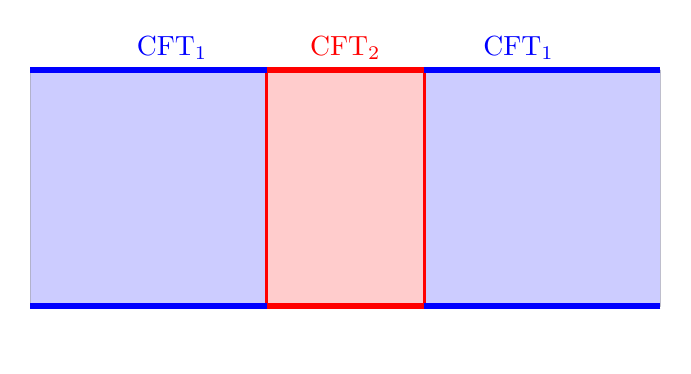
\begin{tikzpicture}
            \draw[fill=blue,opacity=0.2] (-4,3) -- (-1,3) -- (-1,0) -- (-4,0) -- (-4,3);
            \draw[fill=blue,opacity=0.2] (4,3) -- (1,3) -- (1,0) -- (4,0) -- (4,3);
            \draw[fill=red,opacity=0.2] (-1,3) -- (-1,0) -- (1,0) -- (1,3) -- (-1,3);
            \draw[red, line width=2] (-1,3) -- (1,3);
            \draw[red, line width=1] (-1,3) -- (-1,0);
            \draw[red, line width=1] (1,3) -- (1,0);
            \draw[red, line width=2] (-1,0) -- (1,0);
            \draw[blue, line width=2] (-4,3) -- (-1,3);
            \draw[blue, line width=2] (4,3) -- (1,3);
            \draw[blue, line width=2] (-4,0) -- (-1,0);
            \draw[blue, line width=2] (4,0) -- (1,0);
            \filldraw[red] (0,3) circle (0pt) node[anchor=south]{CFT$_2$};
            \filldraw[blue] (-2.2,3) circle (0pt) node[anchor=south]{CFT$_1$};
            \filldraw[blue] (2.2,3) circle (0pt) node[anchor=south]{CFT$_1$};
            \draw[opacity=0] (0,-.5) -- (0,0);
        \end{tikzpicture}
        \caption{}
        \label{itro 1}
     \end{subfigure}
     \hfill
     \begin{subfigure}[b]{0.3\textwidth}
        \centering
        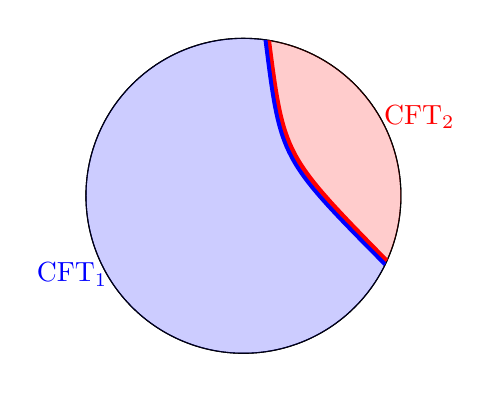
\begin{tikzpicture}
        \draw[name path = A] (1.82,-.829) arc (335.5:440.5:2);
        \draw[name path = AA] (1.82,-.829) arc (335.5:80:2);
            \begin{scope}
                \draw  [clip] (0,0) circle (2cm);
                \draw[color=red,line width=.6mm, name path = B] (1.82,-.829) .. controls (.51,.51) .. (0.32,1.974);
                \draw[color=blue,line width=.5mm, name path = R] (1.80,-.872) .. controls (.47,.47) .. (0.28,1.98);
                \tikzfillbetween[of=A and B]{red, opacity=0.2};
                \tikzfillbetween[of=AA and R]{blue, opacity=0.2};
            \end{scope}
            \draw[red] node at (2,1){~~~~CFT$_2$};
            \draw[blue] node at (-2,-1){CFT$_1$~~~~};
         \end{tikzpicture}
        \caption{}
        \label{intro 2}
     \end{subfigure}
    \caption{(a) Two CFTs separated with a static interface. Time flows upwards. (b) The holographic dual of the two CFTs featuring a domain wall in the bulk separating the two geometries.}
    \label{the intro system}
\end{figure}

All of these important discoveries show that black holes are thermal objects and therefore are not completely black after all. With a temperature different than 0, black holes radiate and evaporate through time as shown by Hawking \cite{Hawking1975}. The essential question behind the evaporation is whether this process can be described under a unitary evolution. According to Hawking's calculations, the thermal entropy of radiations is an increasing function of time, starting at 0 when no Hawking quanta is radiated yet. As the black hole evaporates, the newly emitted radiations grow the entropy until the final stage where the entropy reaches a certain saturation and remains constant.

The increase of the entropy at early stages is expected until it reaches a value equal to one quarter of the area of the horizon. This quantity (\ref{beken}) represents the thermodynamic entropy of the black hole. Surpassing this value would mean that black holes somehow produce information greater than what they store. According to D. Page\cite{PhysRevLett.71.3743}, the von Neumann entropy should start decreasing once it reaches this point, called the Page time, until it reaches 0 at the end of the evaporation process. This decrease of entropy was later understood by means of QES (Quantum Extremal Surface). The von Neumann entropy formula goes as follow\cite{almheiri2020entropy},
\begin{equation}
    S = \text{min}_X\left\{\text{ext}_X\left[\frac{\text{Area}\left(X\right)}{4\hbar G_N} + S_\text{semi-cl}\left(\Sigma_X\right)\right]\right\},
\end{equation}
where $X$ is the QES which we minimize over. Computations result in two extremal surfaces one of which features an island behind the horizon belonging to the radiation slice. This island grows in the heart of the black hole eating up the inside, resulting in an overall decrease of the entanglement entropy.

In this note, we will consider a gravitational system featuring a thin static domain wall separating two geometries as represented in figure \ref{the intro system}. The left and right side of the domain wall are parts of different gravitational solutions: thermal AdS or BTZ black hole. The dual setup consists of two CFTs separated by an interface. This system has been studied in several recent papers\cite{Simidzija_2020, Bachas_2002, DeWolfe_2002}. We follow in this note mainly the analysis presented in \cite{Bachas_2021}. The Einstein-Hilbert action of our toy model is
\begin{equation}\label{action cft}
    \begin{split}
        I = -\frac{1}{2}\int_{\mathbb{S}_1}\text{d}^3x\sqrt{g_1}(R_1&+\frac{2}{\ell_1^2}) -\frac{1}{2}\int_{\mathbb{S}_2}\text{d}^3x\sqrt{g_2}(R_2+\frac{2}{\ell_2^2})\\
        & +\lambda  \int_{\mathbb{W}} \text{d}^2s\sqrt{\hat{g}_\omega} + \text{GHY} + \text{ct.}
    \end{split}
\end{equation}
where $S_i$ is the $i^\text{th}$ slice of the bulk geometry, $g_i$, $R_i$ and $l_i$ respectively its corresponding metric Ricci scalar and AdS radius. The domain wall with an induced metric $\hat{g}$ is described by its tension $\lambda$. The GHY term and the counter-term is computed in \cite{Bachas_2021}.

In particular we are interested in a situation where one slice has a very large number of degrees of freedom compared to the other slice which has a larger border. Following \cite{almheiri2019islands,Almheiri_2020}, we consider our gravitational system to be a finite portion containing the whole slice with the largest central charge. This setup can be described in three alternatives as can be seen in figure \ref{QM fig} where our system of interest is highlighted in yellow.

\begin{figure}
     \centering
     \begin{subfigure}[b]{0.3\textwidth}
        \centering
        \begin{tikzpicture}
            \draw (-2.5,3) -- (2.5,3);
            \draw[yellow, line width=2] (-1.3,3) -- (1.3,3);
            \filldraw[red] (-1,3) circle (2pt) node[anchor=south]{};
            \filldraw[red] (1,3) circle (2pt) node[anchor=south]{};
            \filldraw[red] (0,3) circle (0pt) node[anchor=south]{CFT$_2$};
            \filldraw[blue] (-1.9,3) circle (0pt) node[anchor=south]{CFT$_1$};
            \filldraw[blue] (1.9,3) circle (0pt) node[anchor=south]{CFT$_1$};
            \draw[opacity=0] (0,0) -- (0,3);
        \end{tikzpicture}
        \caption{}
        \label{QM 1}
     \end{subfigure}
     \hfill
     \begin{subfigure}[b]{0.3\textwidth}
         \centering
         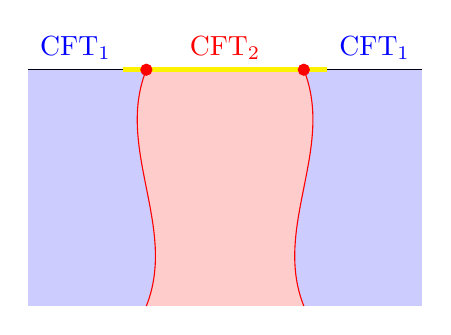
\begin{tikzpicture}
            \draw (-2.5,3) -- (2.5,3);
            \draw[name path = x] (-2.5,3) -- (-1,3);
            \draw[name path = xx] (2.5,3) -- (1,3);
            \draw[name path = xxx] (-1,3) -- (1,3);
            \draw[opacity=0, name path = y] (-2.5,3) -- (-2.5,0) -- (-1,0) .. controls (-.6,1) and (-1.4,2) .. (-1,3);
            \draw[opacity=0, name path = yy] (2.5,3) -- (2.5,0) -- (1,0) .. controls (.6,1) and (1.4,2) .. (1,3);
            \draw[opacity=0, name path = yyy] (-1,3) .. controls (-1.4,2) and (-.6,1) .. (-1,0) -- (1,0) .. controls (.6,1) and (1.4,2) .. (1,3);
            \tikzfillbetween[of= y and x]{blue, opacity=0.2};
            \tikzfillbetween[of= yy and xx]{blue, opacity=0.2};
            \tikzfillbetween[of= yyy and xxx]{red, opacity=0.2};
            \draw[yellow, line width=2] (-1.3,3) -- (1.3,3);
            \filldraw[red] (-1,3) circle (2pt) node[anchor=south]{};
            \filldraw[red] (1,3) circle (2pt) node[anchor=south]{};
            \draw[color=red] (-1,3) .. controls (-1.4,2) and (-.6,1) .. (-1,0);
            \draw[color=red] (1,3) .. controls (1.4,2) and (.6,1) .. (1,0);
            \filldraw[red] (0,3) circle (0pt) node[anchor=south]{CFT$_2$};
            \filldraw[blue] (-1.9,3) circle (0pt) node[anchor=south]{CFT$_1$};
            \filldraw[blue] (1.9,3) circle (0pt) node[anchor=south]{CFT$_1$};
    \end{tikzpicture}
         \caption{}
         \label{QM 2}
     \end{subfigure}
     \hfill
     \begin{subfigure}[b]{0.3\textwidth}
         \centering
         \begin{tikzpicture}
            \draw (0,3) -- (4,3);
            \filldraw[yellow] (0,3) circle (5pt) node[anchor=south]{QM};
            \draw[yellow, line width=2] (0,3) -- (1,3);
            \draw (1,2.8) -- (1,3.2);
            \draw (.9,2.8) -- (1,2.8);
            \draw (.9,3.2) -- (1,3.2);
            \draw[opacity=0] (0,0) -- (0,3);
            \filldraw[blue] (3,3) circle (0pt) node[anchor=south]{CFT$_1$};
        \end{tikzpicture}
         \caption{}
         \label{QM 3}
     \end{subfigure}
     \hfill
    \caption{(a) CFT$_1$  and CFT$_2$ respectively with central charges $c_1\ll c_2$ and boundaries $L_1\gg L_2$. These are separated by an interface shown in red circles. (b) The holographic dual of the two CFTs featuring a domain wall with tension $\lambda$ separating between the two geometries. (c) Our gravitational system with large degrees of freedom represented by a quantum dot following the central dogma, with a small slice of the bath region.}
    \label{QM fig}
\end{figure}

The goal of this study is to study the behaviour of the entanglement entropy of the yellow region. This will require purifying the thermal state by virtue of the thermofield double state, dual to the double sided  geometry\cite{ISRAEL1976107}. The computation of  RT surfaces will follow. We expect a rising entropy as a function of time, and a saturating constant entropy at late times.

This note is organised as follows. In chapter \ref{section 2} we present a review of entanglement entropy in the frame work of quantum mechanics as well as field theory. In chapter \ref{section 3}, we review the holographic computation of entanglement entropy proposed by S. Ryu and T. Takayanagi\cite{Ryu, Ryu_2006} with explicit calculations for two examples: vacuum CFT and BTZ black hole. In chapter \ref{section 4} we present briefly the thermodynamic equations behind black hole dynamics. We summarise Hawking information paradox as well as its solution by means of QES. In chapter \ref{section 5} we review the work presented in \cite{Bachas_2021} regarding Holographic ICFTs. We then consider the limit of interest with a large bath $L_1\gg L_2$ and large degrees of freedom in the other side $c_1\ll c_2$. We find the dominant phase and pursue its study in the next chapter \ref{section 6}. We compute the RT surfaces through geodesic calculations. In chapter \ref{section 7} we give the double sided geometry of the dominant phase, dual to a pure CFT state living on its double boundary. We then compute RT surfaces in the double sided geometry. We find that the entropy of our system follows a Page curve. 


\addchap{Entanglement Entropy}
\setcounter{chapter}{1}
\refstepcounter{chapter}
\label{section 2}
For the sake of completeness, we recall here some standard definitions and properties about entanglement entropy. We also take the opportunity to set some notations and conventions that will be used throughout this report. This review is mainly based on chapter 2 and 3 of Matthew Headrick's lecture \cite{entropy}.

\section{Von Neumann entropy}

One of the ultimate differences between classical and quantum mechanics is that in quantum mechanics one can not separate between the notion of state of a system and the knowledge we have on the state of the system. In quantum mechanics, we encode this information in an operator named \textbf{density matrix} obeying the following:
\begin{align}\label{properties of rho}
    \rho^\dagger = \rho,         &&           \rho \geq 0,          &&        \text{Tr}\rho=1.
\end{align}

We distinguish between two types of states. A state is called \textbf{pure} if it can be written as a one dimensional projector,
\begin{equation}\label{pure state}
    \rho = \ket{\psi}\bra{\psi}.
\end{equation}
In this case, $\rho$ cannot be written as a linear combination of other states. The expectation value of observables simply takes the form $\Braket{A}=\bra{\psi}A\ket{\psi}$.

The rest of the states are \textbf{mixed}. These are statistical ensembles of pure states. One way to distinguish between pure and mixed states is by computing $\text{Tr}\rho^2$. This trace is obviously equal to 1 in the case of (\ref{pure state}) and is less than 1 for mixed states. Geometrically, pure states are represented as vectors on the surface of the Bloch-Sphere whilst mixed states are represented with vectors inside the sphere.

It is important to note that, using (\ref{properties of rho}), the density matrix can be diagonalized,
\begin{equation}
    \rho = \sum_a p_a\ket{a}\bra{a}
\end{equation}
where $p_a$ is a probability distribution.

The entropy of the state $\rho$ comes natural from the \textit{Shannon entropy} in the classical case \cite{bengtsson_zyczkowski_2006},
\begin{equation}\label{Von Neumann}
    S\left(\rho\right):=S\left(\Vec{p}\right)=-\text{Tr}\rho\ln \rho = \braket{-\ln\rho}_\rho.
\end{equation}
This is known as the \textbf{Von Neumann entropy}. It is non negative and vanishes if and only if $\rho$ is a pure state. It is also invariant under unitary transformation, i.e unitary transformations are reversible.

Things get more interesting when we consider a joint system $AB$. The Hilbert space of the joint system is
\begin{equation}
    \mathcal{H}_{AB}\cong \mathcal{H}_A\otimes\mathcal{H}_B    
\end{equation}
where $\cong$ means isomorphic (same structure). We can always find the state of the subsystem $A$ by taking the trace over $B$,
\begin{equation}
    \rho_A := \text{Tr}_B\rho_{AB}.
\end{equation}
This is the \textbf{reduced density matrix}. The Von Neumann entropy (\ref{Von Neumann}) is extensive and subadditive,
\begin{equation}
    S\left(AB\right) \leq S\left(A\right) + S\left(B\right)
\end{equation}

There are two other important inequalities that are obeyed by the entropies of subsystems. The first one is the \textbf{Araki-Lieb} inequality,
\begin{equation}\label{Araki-Lieb}
    S\left(AB\right) \geq \left|S\left(A\right) - S\left(B\right)\right|
\end{equation}
and the second called the \textbf{strong subadditivity},
\begin{equation}\label{weak monotonicity}
    S\left(AB\right) + S\left(BC\right) \geq S\left(A\right) + S\left(C\right).
\end{equation}

An important result of (\ref{Araki-Lieb}) is that $S\left(A\right) = S\left(B\right)$ if $AB$ is a pure state.

\section{Entanglement}
There has been many works in the area of quantum entanglement measurements. Entanglement entropy is the main measurement tool to quantify entanglement, especially in the case of pure states. But there are many considerable different ways to quantify the amount of entanglement like the entanglement cost, distillable entanglement or entanglement of formation \cite{Virmani}.

Entanglement entropy  is a measure of how quantum information is spatially organised in a quantum state. We distinguish between two cases: $AB$ pure and $AB$ mixed.

\subsection{Pure state}
A pure state (\ref{pure state}) that cannot be factorized into the product of two,
\begin{equation}\label{factorized state}
    \ket{\psi} = \ket{\psi'}_A\otime\ket{\psi''}_B
\end{equation}
is \textbf{entangled}. One can consider the famous example of a \textbf{Bell pair} \cite{Bell}, a qubit bipartite system $AB$ in the pure state
\begin{equation}\label{Bell pair}
    \ket{\psi}=\frac{1}{\sqrt{2}}\left(\ket{0}_A\otimes\ket{1}_B+ \ket{1}_A\otimes\ket{0}_B\right).
\end{equation}
We can verify the entanglement of $A$ and $B$ by computing their corresponding entanglement entropy through their reduced density matrix (\ref{psiA}), see Appendix \ref{appendix A}. If it is different than zero then the subsystems are mixed which indicates that they are entangled.
\begin{equation}\label{psiA}
    \rho_A := \text{Tr}_B\rho = \frac{1}{2}\left(\ket{0}_A\bra{0}+\ket{1}_A\bra{1}\right)
\end{equation}
There is a connection between entanglement and factorization in the case of a pure state. The state $\rho_{AB}$ can be factorized if and only if $\rho_A$ is pure, which is true if and only if $\rho_B$ is pure. An important fact to mention is that if we start with an unentangled state $\rho_{AB}$, no combination of \textit{local operations} on $A$ and $B$ and no \textit{classical communication} between $A$ and $B$ (\textbf{LOCC})  will result in a pure entangled state. In other words, if the two subsystems $A$ and $B$ are to be entangled, it requires the action of a third party.

Entropies are bounded by the log of the dimension of their Hilbert space. This is obvious following the definition (\ref{Von Neumann}). In the limit of a large Hilbert space, this bound becomes saturated and we have,
\begin{equation}
    S\left(A\right) = \min \left\{ \ln\dim\mathcal{H}_A,\ln\dim\mathcal{H}_B\right\} + \mathcal{O}(1).
\end{equation}

As an example, if $AB$ is a system of large number of spins where a touch $x$ is part of $A$ and the rest belongs to $B$, then the entanglement entropy follows what we call a \textbf{Page curve} as a function of $x$, fig. \ref{page curve}. At the start, the Page curve was a model used in black hole physics, being considered in pure state at $t_0$, to understand its evaporation process. The subsystem $A$ containing the black hole becomes entangled with outgoing Hawking radiations $B$ throughout the evaporation process. The Black hole's EE is supposed to follow a Page curve.

\begin{figure}
    \centering
    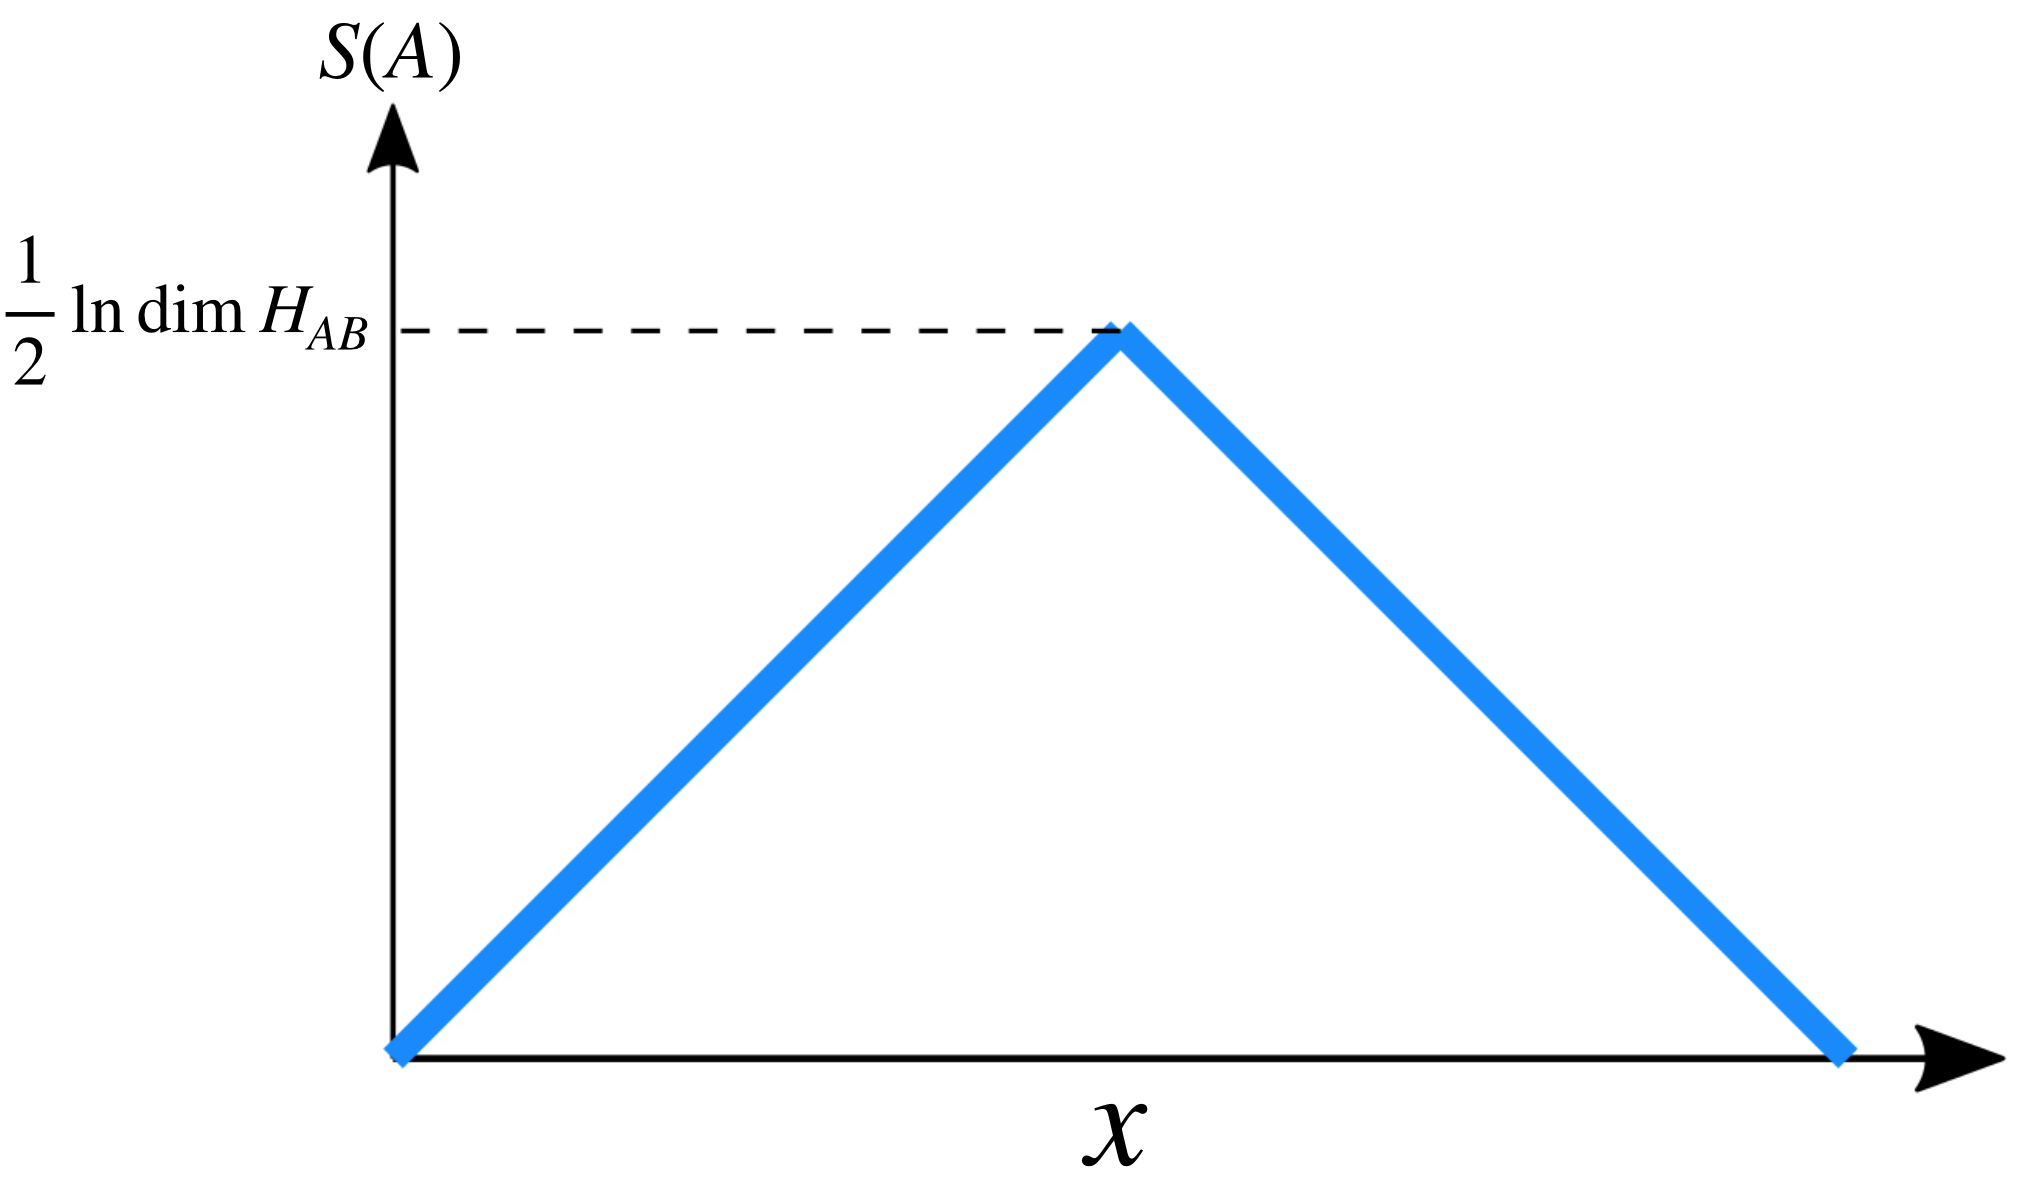
\includegraphics[width=0.65\textwidth]{figures/page_curve.png}
    \caption{The EE $S(A)$ of a subset $A$ of a larger system $AB$ in a pure state. $AB$ is a system of large spins where a fraction $x$ of them belongs to $A$. The EE follows a Page curve.}
    \label{page curve}
\end{figure}

\subsection{Mixed state}
In the case of mixed states, the results mentioned in the previous subsection are almost lost. We say that a state is not entangled if it is separable (classically correlated), i.e
\begin{equation}
    \rho = \sum_ip_i{\rho^i}_A\otimes{\rho^i}_B.
\end{equation}

Detecting entanglement and its type (classical or quantum) turns out to be a very (NP-)hard problem\cite{gharibian2009strong}. One way to detect this entanglement is to compute the sign of the \textbf{conditional entropy}
\begin{equation}\label{conditional entropy}
    H\left(A|B\right):=S\left(AB\right)-S\left(B\right)
\end{equation}
which is positive in the classical case and for separable states. This condition is sometimes violated in the presence of entanglement, like in the case of an entangled pure state,
\begin{equation}\label{negative H(A|B)}
    H\left(A|B\right) = -S\left(B\right)\leq 0.
\end{equation}

\subsection{Monogamy of entanglement}

One last feature we mention on entanglement is the property of monogamy. This comes from the strong subadditivity (\ref{weak monotonicity}) which can be rewritten as (see Appendix \ref{appendix A}),
\begin{equation}\label{SSA}
     H\left(B|A\right) + H\left(B|C\right)\geq 0.
\end{equation}
This shows that at most, one of the pairs $AB$ or $CB$ can be entangled.

In the case of black hole evaporation, this monogamy represents an issue. Consider a black hole at a time $t$ where more than half of the radiation has been emitted. The next outgoing Hawking quanta "$B$" will be entangled with those previously emitted "$A$" while at the same time it is entangled with ingoing particles "$C$". Many explanations have been suggested to solve this paradox. One proposition by AMPS\cite{Almheiri_2013} suggested a firewall at the horizon shielding the falling observers from entering the black hole. This proposal was criticized as it violates Einstein's equivalence principal. Maldacena and Susskind \cite{Maldacena_2013} proposed in ER=EPR that outgoing and ingoing Hawking quanta are connected through a wormhole and as a result should not be considered as independent systems.

\section{Thermofield double}

Mixed states can always be considered to be part of a larger system $\Tilde{H} = H\otimes K$ which is in a pure state. To get back the original system, we can trace over the complement system $K$. This method goes under the name of purification \cite{Kleinmann_2006}.

One way to perform this purification is through the \textbf{thermofield double}.  In this method, the pure state is created by doubling the original system $A$. Consider for example a \textbf{Gibbs state}
\begin{equation}\label{Gibbs state}
    \rho_A = \frac{1}{Z}\sum_a e^{-\beta E_a}\ket{a}_A\bra{a}.
\end{equation}
We choose $K$ to be a copy of the original system $\mathcal{H}_A$. The thermofield double state is
\begin{equation}\label{thermofield double}
    \ket{\phi} = \frac{1}{\sqrt{Z}}\sum_a e^{-\beta E_a/2}\ket{a}_A\otimes\ket{a}_B.
\end{equation}

If the purification was made by a different system, the resulting state $\ket{\chi}$ is related to the thermofield double by a unitary transformation,
\begin{equation}
    \ket{\chi} = I_A\otimes U_B \ket{\phi}.    
\end{equation}
This is known as the Schrödinger–HJW theorem, \cite{schrodinger_1936}.

The thermofield double state can be written in terms of an Euclidean path integral on a semicircle of length $\beta/2$. This can be seen if we write the operator $e^{-\beta H}$ as an Euclidean path integral over an interval of length $\beta$. It's matrix element is a path integral with boundary conditions and can be represented as
\begin{equation}\label{l3iba}
    \bra{x_0}e^{-\beta H}\ket{x_1} = \ctikz{\draw (0.967,0.255) arc (10:350:1);\node at (0.967,0.255) [circle,fill=red,inner sep=1.5pt]{}; \node at (0.96,-0.150) [circle,fill=red,inner sep=1.5pt]{};
    \draw node at (1.3,-0.2){$x_0$};\draw node at (1.3,0.2){$x_1$};},
\end{equation}
where the circle is of length $\beta$. The component of the thermofield double state in $\ket{x_a}\otimes\ket{x_b}$ is
\begin{equation}
    \left(\bra{x_a}\otimes\bra{x_b}\right)\ket{\phi} = \frac1{\sqrt{Z}} \times \ctikz{\draw (-1,0) arc (180:360:1);\node at (-1,0) [circle,fill=red,inner sep=1.5pt]{}; \node at (1,0) [circle,fill=red,inner sep=1.5pt]{};
    \draw node at (-1.3,0){$x_0$};\draw node at (1.3,0){$x_1$};}.
\end{equation}
where the circle is of length $\beta/2$. One can check that tracing (\ref{thermofield double}) gives back exactly the original Gibbs state (\ref{Gibbs state}). This can also be checked in the path integral formulation as done in appendix \ref{appendix A}. This shows how thermal states are originated from entanglement in a larger system.

\section{Fine-grained vs Coarse-grained entropy}

There are two notions of entropy that will be of use in the following chapters: fine-grained and coarse-grained entropy.

The fine-grained entropy is the von Neumann entropy (\ref{Von Neumann}) we discussed above. As we mentioned earlier, it quantifies our ignorance on the system and most importantly it is invariant under unitary evolution $\rho\rightarrow U\rho U^{-1}$.

The coarse-grained entropy is defined as follows. Having a density matrix $\rho$ that describes our system, we consider all possible states $\Tilde{\rho}$ such that the subset of observables $A_i$ that we are considering is unchanged, $\text{Tr}[\Tilde{\rho}A_i]=\text{Tr}[\rho A_i]$. Then we maximize the von Neumann entropy over $\Tilde{\rho}$. This definition increases with unitary time evolution and therefore obeys the second law of thermodynamics. 

One important point to mention, though obvious, is that the fine-grained entropy is always smaller than the coarse-grained entropy by definition,
\begin{equation}
    S_{vN}\leq S_{\text{coarse}}.    
\end{equation}

A simple example of the coarse-grained entropy is the thermodynamic entropy, where the observables subset contains energy and volume.

\section{Entanglement entropy in Field theories}

One can consider field theories to be the limit of lattice systems where the lattice spacing goes to zero $a\rightarrow0$ to obtain a continuous spacial region as shown in fig. \ref{lattice system}. The Hilbert space of such a system is the direct product of local Hilbert spaces,
\begin{equation}
    \mathcal{H} = \otimes_{x}\mathcal{H}_x.
\end{equation}

In relativistic quantum field theory, this spacial region can be replaced by a Cauchy slice $\sigma$. Since observables on Cauchy slices in different points commute, a region $A\in\sigma$ comes with a factorization of the Hilbert space as
\begin{equation}
    \mathcal{H} = \mathcal{H}_{A} \otimes \mathcal{H}_{A^c},
\end{equation}
up to some technicalities in the entanglement surface. This spacial region has the same entropy as any other region that shares with $A$ the same causal domain $D(A)$\footnote{The caudal domain $D(A)$ of a region $A$ is the group of all the points that are only causally related to $A$.},
\begin{equation}
    D(A) = D(A') \implies S(A) = S(A').
\end{equation}

\begin{figure}
    \centering
    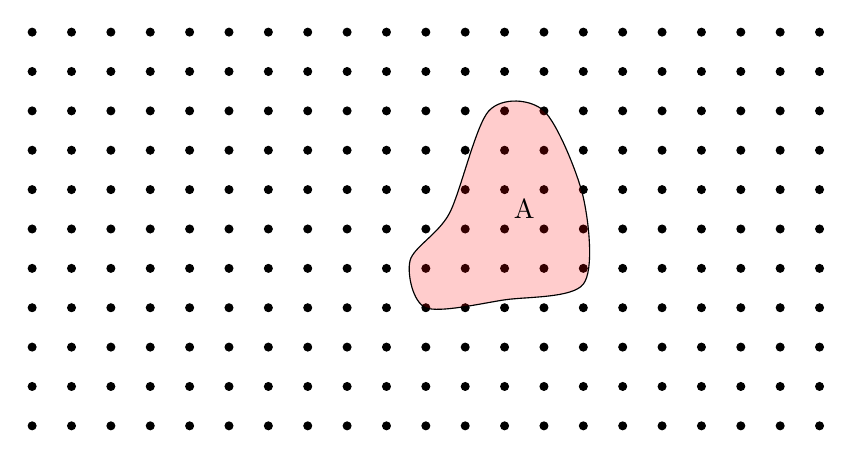
\begin{tikzpicture}
        [%%%%%%%%%%%%%%%%%%%%%%%%%%%%%%
            dot/.style={circle,draw=black, fill,inner sep=1pt},
        ]%%%%%%%%%%%%%%%%%%%%%%%%%%%%%%
        
        \foreach \x in {0,...,20}{
            \foreach \y in {0,...,10}{
                \node[dot] at (\x/2,\y/2){ };
            }
        }

        \draw[fill=red,opacity=0.2] plot [smooth cycle] coordinates {(5,1.5) (6,1.6) (7,1.8) (7,2.9) (6.5,4) (5.8,4) (5.3,2.7) (4.8,2.1) } node at (6,2.5){};
        \draw plot [smooth cycle] coordinates {(5,1.5) (6,1.6) (7,1.8) (7,2.9) (6.5,4) (5.8,4) (5.3,2.7) (4.8,2.1) } node at (6.25,2.75){A};
    \end{tikzpicture}
    \caption{Region $A$ of a lattice system with lattice spacing $a$.}
    \label{lattice system}
\end{figure}

Entanglement entropies in field theories are usually computed using path integrals and the replica trick (which consists of considering $n$ replica of the original system). However, for theories that admit holographic description (in the sense of AdS/CFT correspondence), entanglement entropies can be found through a simple computation of minimal surfaces. This will be the subject of the next chapter. 


\addchap{Entanglement Entropy in Holographic Theories}
\setcounter{chapter}{2}
\refstepcounter{chapter}
\label{section 3}
In the previous section we've seen various definitions and properties regarding entanglement entropies. One problem we might have is that these quantities are rather difficult, sometimes impossible, to compute.

Holographic theories are an exception to this rule. We can compute EE in holographic theories simply by solving a geometric problem. This is known as the Ryu-Takayanagi (RT) formula, \cite{Ryu, Ryu_2006}.

This chapter is based on Matthew Headrick's lecture \cite{entropy} and Thomas Hartman's lecture \cite{TomHartman}.

\section{Ryu-Takayanagi formula}
In holographic theories- describing $d-$dimensional quantum field theories to $d+1-$dimensional quantum gravity with negative cosmological constant- it is possible to compute the EE geometrically. This is known as the \textbf{Ryu-Takayanagi (RT) formula}. This formula makes a connection between the bulk geometry and spatial entanglement. It is a generalization of the famous \textbf{Bekenstein-Hawking entropy}, \cite{PhysRevD.7.2333, PhysRevLett.26.1344},
\begin{equation}\label{Bekenstein-Hawking}
    S_{\text{BH}}= \frac{1}{4G_\text{N}}\text{area}\left(m_{\text{hor}}\right),
\end{equation}
which expresses the entropy of a black hole with $m_{hor}$ the area of its bifurcate horizon ($\hbar=1$). 

As $S_{\text{BH}}$ is a thermal entropy, this system can be purified using the thermofield double (\ref{thermofield double}). The two copies of the system are two duplicates of the field theory on the spacetime boundary $M\cup M'$, see fig. \ref{Penrose diagram thermofield double}. It's holographic representation is the extended symmetric two sided black hole space time \cite{ISRAEL1976107, PhysRevD.48.1506}, where the original thermal system is its right exterior region.

Consider a bulk Cauchy slice $\sigma$ which intersects the boundary at the boundary Cauchy slice $A\cup A^c$ as shown in fig. \ref{Penrose diagram thermofield double}. In this new purified system, the entropy of the right boundary Cauchy slice $S(\rho_A)$ is equal to that of its complement $A_c$ (the left boundary Cauchy slice) which in turn is equal to the thermal entropy of the original system,
\begin{equation}\label{BH A = Ac}
    S\left(A_c\right) = S\left(A\right) = \frac{\text{area}\left(m_{\text{hor}}\right)}{4G_\text{N}}.
\end{equation}

This formula could be related to situations where there isn't necessarily a black hole. The area of the horizon $m_\text{hor}$ in (\ref{BH A = Ac}) can be regarded as the minimal surface separating two regions $r(A)$, bounded by $A$, and $r(A^c)$ bounded by $A^c$\footnote{In fig. \ref{Penrose diagram thermofield double}, this is the right and left red segments.}. In the absence of a horizon a natural generalisation is to replace $m_\text{hor}$ with the minimal bulk surface separating $A$ and $A^c$. This minimal area feature that relates the surface $m$ to the entropy $S(A)$ is what is know as the RT formula,
\begin{equation}\label{RT}
    S\left(A\right)= \frac{1}{4G_\text{N}}\min_{m\sim A}\text{area}\left(m\right),
\end{equation}
where $m\sim A$ means homologous to $A$\footnote{We say an oriented surface $m$ is homologous to $A$ if there exist a region $r$ in the bulk Cauchy slice such that $\partial r = A\cup -m$.}.

In 2006, S. Ryu and T. Takayanagi showed how one can recover the entropy of $d-$holographic quantum field theories using a formula analogous to that of Bekenstein-Hawking (\ref{Bekenstein-Hawking}), \cite{Ryu}. In this formulation, one can also compute EE of a partial region $B\subset A$. The horizon surface is replaced by a holographic $d$ dimensional minimal surface whose boundary is $\partial B$, where $B$ is the CFT subsystem we are interested in. This result is quite impressive as it allow us to compute CFT entropies using surfaces even in the absence of a horizon in the holographic gravitational solution. The statement proposed by Ryu and Takayanagi is another strong evidence of the AdS/CFT correspondence conjectured by Maldacena, \cite{Maldacena_1999}.

\begin{figure}
    \centering
    \begin{tikzpicture}\label{2d Penrose diag}
    \node (I)    at ( 3,0)   {I~~~~~~~~~~~~~~~};
    \node (II)   at (-3,0)   {~~~~~~~~~~~~~~~II};
    \node (III)  at (0, 1) {III};
    \node (IV)   at (0,-1) {IV};
        
    \path  % Four corners of left diamond
         (II) +(90:3)  coordinate[label=90:$i^+$]  (IItop)
         + (0:0) coordinate[label=180:$A^c$] (IImid)
         +(-90:3) coordinate[label=-90:$i^-$] (IIbot)
         +(0:3)   coordinate                  (IIright)
               ;
    \draw (IItop) --
        node[midway, below, sloped] {$\bar{u}=0$}
        (IIright) -- 
        node[midway, below, sloped] {$\bar{u}=0$}
        (IIbot) --
        node[midway, above, sloped] {$r=\infty$}
        (IImid) --
        (IItop) -- cycle;
        
    \path % Four conners of the right diamond (no labels this time)
        (I) +(90:3)  coordinate (Itop)
        + (0:0) coordinate[label=0:$A$] (Imid)
        +(-90:3) coordinate (Ibot)
        +(180:3) coordinate (Ileft);
        % No text this time in the next diagram
    \draw  (Ileft) -- (Itop) -- node[midway, above,     sloped] {$r=\infty$} (Imid) -- (Ibot) -- (Ileft) --        cycle;
      
    \draw[thick,red,-] (IImid) -- (Imid) --; 
      
    % Squiggly lines
    \draw[decorate,decoration=zigzag] (IItop) --         (Itop)
        node[midway, above, inner sep=2mm] {$r=0$};
        
    \draw[decorate,decoration=zigzag] (IIbot) --         (Ibot)
        node[midway, below, inner sep=2mm] {$r=0$};
    
    \node[circle,draw=black, fill=red, inner sep=0pt,minimum size=5pt] (Ileft) {};
    \draw node at (-3.4,2.6){$M'$};
    \draw node at (3.4,2.6){$M$};
    \end{tikzpicture}
    \caption{2 dimensional Penrose diagram of the BTZ geometry (equation (\ref{geometry}) with positive mass). The red line is the time reflection invariant bulk Cauchy slice with $A$ and $A^c$ its conformal boundaries. The compactification is performed explicitly in section \ref{section 8}.}
    \label{Penrose diagram thermofield double}
\end{figure} 

Originally, the R-T formula (\ref{RT}) was derived to compute entanglement entropy in AdS spacetime. But it goes beyond that: It requires no entanglement, no holography and no AdS neither \cite{Hubeny_2007}.

\section{Examples}

In this section we present two examples which will be of use in the following chapters. Part of the computations are presented in the appendix as well as chapter \ref{section 6}.

\subsection{CFT vacuum}

Consider a two-dimensional CFT, dual to AdS$_3$ with the metric
\begin{equation}\label{AdS_3 metric}
    \text{d}s^2= \frac{\ell^2}{z^2}\left(-\text{d}t^2+\text{d}x^2+\text{d}z^2\right),
\end{equation}
where $\ell$ is the AdS radius related to cosmological constant $\Lambda = -\frac{1}{2}d(d-1)\ell^{-2}$.

We want to compute the entanglement entropy of an interval $A\subset$ the boundary. This goes back to computing RT surfaces $m$ that are homologous to $A$. These are codimension-2 surfaces in AdS$_3$, and therefore $1-$dimensional, so a geodesic.

Solving the Einstein field equations\footnote{Detailed computations in Appendix \ref{appendix B}.}, we find the geodesics to be semicircles ($z\geq 0$) with their center lying on the boundary,
\begin{equation}\label{AdS_3 vaccum geodesic}
    \left(x-x_0\right)^2+z^2=r^2.
\end{equation}

The $1/z^2$ term in the metric $\left(\ref{AdS_3 metric}\right)$ will make the geodesic diverge on the boundary. This is the gravity dual of the divergence of QFT entanglement entropy. We deal with this UV divergence by introducing a cutoff at $z=\epsilon$.

\begin{figure}
    \centering
    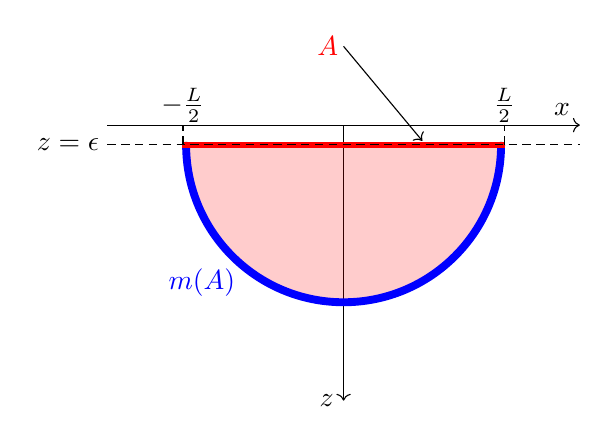
\begin{tikzpicture}[
        circ/.style={circle, draw, solid, fill=white, inner sep=0.75pt,
                     label=#1,
                     node contents={}
                     },
        every label/.append style = {inner sep=2pt, font=\footnotesize}
                            ]
        % shaded area
        
        % axis
        \draw[->]   (-6,0) -- + (6,0) node[above left] {$x$};
        \draw[->]   (-3,0) -- + (0,-3.5) node[left] {$z$};
        % rest of image
        \draw[fill=red,opacity=0.2] (-5,-.25) node[circ=below left:] arc (180:360:2) node[circ=below right:{}];
        \draw node at (-.96,.25){$\frac{L}{2}$};
        \draw node at (-5.04,.25){$-\frac{L}{2}$};
        \draw[blue, line width=1mm] (-5,-.25) arc (180:360:2);
        \draw[red, line width=.75mm] (-5.05,-0.25) -- (-.95,-0.25);
        %
        \draw[densely dashed]   (-5.04,-0.25) -- (-5.04,0);
        \draw[densely dashed]   (-.96,-0.25) -- (-.96,0);
        \draw[densely dashed]   (-6,-0.25) -- (0,-0.25);
        \draw node at (-6.5,-0.25){$z=\epsilon$};
        \draw[blue] node at (-4.8,-2.){$m(A)$};
        \draw[red] node at (-3.2,1){$A$};
        \draw[->]   (-3,1) -- + (1,-1.2);
    \end{tikzpicture}
    \caption{The blue curve represents the minimal bulk surface homologous to $A$ the red boundary slice. The dashed line is the z cutoff to prevent from UV divergences.}
    \label{Vacuum AdS}
\end{figure}

Consider a region $x\in\left[-L/2,+L/2\right]$ on the cutoff surface as presented in fig. \ref{Vacuum AdS},
\begin{align}
    x_0 = 0,        &&      r^2 = \left(\frac{L}{2}\right)^2+\epsilon^2.
\end{align}
Using (\ref{AdS_3 metric}) and (\ref{AdS_3 vaccum geodesic}), the length of the surface linking the two endpoints is easily computed and is found to be
\begin{equation}\label{first RT}
    m\left(A\right) = 2\ell\ln\left(\frac{L}{\epsilon}\right).
\end{equation}
Plugging this into the RT formula (\ref{RT}), and using the relation between the central charge and the AdS radius\footnote{In the limit of large number of field-theory degrees of freedom this relation is $c=\frac{3}{2G_\text{N}}\ell$.}, the entropy is
\begin{equation}
    S\left(A\right)= \frac{c}{3}\ln\left(\frac{L}{\epsilon}\right).
\end{equation}

The logarithmic divergence is expected from the term $\text{d}s\sim \ell \text{d}z/z$ in the metric.

\subsection{Holographic entanglement at finite temperature}

Now we derive the entanglement entropy of an interval on a circle $\Sigma$ of radius $R$, on which lives a CFT dual to a BTZ black hole in AdS$_3$.

Consider a holographic CFT on a circle $\Sigma$ of radius $R$. This system undergoes a \textbf{Hawking-Page} transition at temperature $T^*=\left(2\pi R\right)^{-1}$, \cite{Hawking1983}. This can be seen by comparing the free energies of the two possible geometries: thermal AdS and BTZ black hole. 
\begin{equation}
    \Delta F = F_{AdS}-F_{BTZ} = 2\pi^2\ell(LT^2-\frac{1}{L}),
\end{equation}
where $L=2\pi R$. Above this temperature, the bulk becomes a BTZ Black hole\cite{Ba_ados_1992},
\begin{align}\label{BTZ}
    \text{d}s^2 = \frac{\ell^2}{z^2}\left(-f\left(z\right)\text{d}t^2+\text{d}x^2+\frac{\text{d}z^2}{f\left(z\right)}\right),     &&      f\left(z\right)=1-\frac{z^2}{z_h^2}.
\end{align}
where $z_h$ is the position of the horizon and $x\sim x+2\pi R$. Using a Wick rotation $\tau=it$, we can show that $z_h$ is related to the Hawking temperature, see Appendix \ref{appendix B}.
\begin{equation}\label{Haking temperature}
    T = \frac{1}{2\pi z_h}.
\end{equation}

As the RT formula was introduced for pure states, it is not supposed to apply directly for the thermal state $\rho_\Sigma$. One should purify the state. One way to do this is through the thermofield double state, dual to the two-sided BTZ black hole, fig. \ref{Penrose diagram thermofield double}. But there are many other options to purify the thermal state as discussed in the previous chapter. This might be a problem if the minimal surface $m(A)$ depends on the choice of the purification. However, RT avoids this problem by a property called nesting. This property states that for any regions $A$ and $B$,
\begin{equation}
    r\left(A\right) \subseteq r\left(AB\right) = \sigma,
\end{equation}
where $r(A)$ is the the homology region of $A$. In this case the choice of purification is irrelevant. The nesting condition is but a geometric way to say that the state of a larger system determines the state of it subsystems.

However, there is one important equation that does not hold in the case of a thermal state,
\begin{equation}
    S\left(A\right)\neq S\left(A^c\right),
\end{equation}
which is what we should expect for a mixed state anyway.

\begin{figure}
     \centering
     \begin{subfigure}[b]{0.3\textwidth}
        \centering
        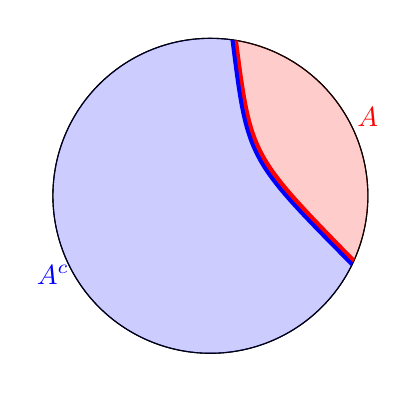
\begin{tikzpicture}
        \draw[name path = A] (1.82,-.829) arc (335.5:440.5:2);
        \draw[name path = AA] (1.82,-.829) arc (335.5:80:2);
            \begin{scope}
                \draw  [clip] (0,0) circle (2cm);
                \draw[color=red,line width=.6mm, name path = B] (1.82,-.829) .. controls (.51,.51) .. (0.32,1.974);
                \draw[color=blue,line width=.5mm, name path = R] (1.80,-.872) .. controls (.47,.47) .. (0.28,1.98);
                \tikzfillbetween[of=A and B]{red, opacity=0.2};
                \tikzfillbetween[of=AA and R]{blue, opacity=0.2};
            \end{scope}
            \draw[red] node at (2,1){$A$};
            \draw[blue] node at (-2,-1){$A^c$};
         \end{tikzpicture}
         \caption{}
         \label{fig_BTZ minimal surface a}
     \end{subfigure}
     \hfill
     \begin{subfigure}[b]{0.3\textwidth}
         \centering
         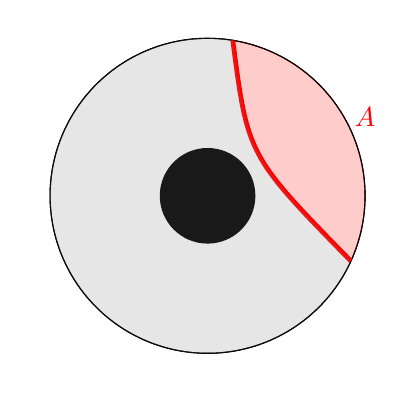
\begin{tikzpicture}
            \draw[name path = A] (1.82,-.829) arc (335.5:440.5:2);
            \draw[name path = AA] (1.82,-.829) arc (335.5:80:2);
            \draw[black,fill=black] (0,0) circle (.6cm);
            \begin{scope}
                \draw  [clip] (0,0) circle (2cm);
                \draw[color=red,line width=.6mm, name path = B] (1.82,-.829) .. controls (.51,.51) .. (0.32,1.974);
                \tikzfillbetween[of=A and B]{red, opacity=0.2};
                \tikzfillbetween[of=AA and B]{gray, opacity=0.2};
            \end{scope}
            \draw[red] node at (2,1){$A$};
         \end{tikzpicture}
         \caption{}
         \label{fig_BTZ minimal surface b}
     \end{subfigure}
     \hfill
     \begin{subfigure}[b]{0.3\textwidth}
         \centering
         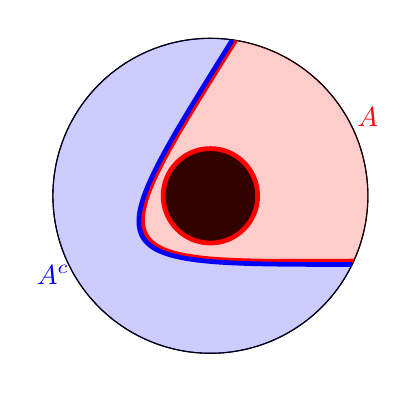
\begin{tikzpicture}
            \draw[name path = A] (1.82,-.829) arc (335.5:440.5:2);
            \draw[name path = AA] (1.82,-.829) arc (335.5:80:2);
            \draw[red,fill=black,line width= .6mm] (0,0) circle (.6cm);
            \begin{scope}
                \draw  [clip] (0,0) circle (2cm);
                \draw[color=red,line width=.6mm, name path = B] (1.82,-.829) .. controls (-1.45,-.85) .. (0.32,1.974);
                \draw[color=blue,line width=.6mm, name path = R] (1.80,-.872) .. controls (-1.5,-.87) .. (0.28,1.98);
                \tikzfillbetween[of=A and B]{red, opacity=0.2};
                \tikzfillbetween[of=AA and R]{blue, opacity=0.2};
            \end{scope}
            \draw[red] node at (2,1){$A$};
            \draw[blue] node at (-2,-1){$A^c$};
         \end{tikzpicture}
         \caption{}
         \label{fig_BTZ minimal surface c}
     \end{subfigure}
     \hfill
    \caption{RT surfaces for a (a) pure state, and a (b,c) thermal state. In the case of a horizon in the bulk, there are many geodesics homologous to $A$. The choice between (b) and (c) is a result of minimizing the surface. This choice results in a sort of Page curve \ref{BTZ entropy phase transition}.}
    \label{fig_BTZ minimal surface}
\end{figure}

In the presence of a black hole, there are several possibilities regarding minimal surfaces as it can be seen in fig. \ref{fig_BTZ minimal surface}. As a matter of fact, there are an infinite number of geodesics indexed with their winding number around the black hole. Defining the region $A$ to be the boundary segment $\phi\in(0,L)$,  in the case $L\ll2\pi $, the obvious choice is that represented in fig. \ref{fig_BTZ minimal surface b}. It's length is
\begin{equation}\label{length BTZ red}
    2\ell\ln\frac{\sinh\left(\pi T L\right)}{\pi T\epsilon}.
\end{equation}
This result can be found by computing geodesics in a BTZ background as will be done in chapter \ref{section 6}.

In the case of large $L$, a second choice \ref{fig_BTZ minimal surface c} becomes possible as well. The geodesic winds (maybe multiple times) around the horizon. If we consider just the blue geodesic in fig. \ref{fig_BTZ minimal surface c}, $A$ does no longer satisfy the homology condition (we cannot continuously deform the geodesic to $A$), unless we add to it the horizon. In this case the minimal surface is,
\begin{equation}
    m\left(A\right) = m\left(A^c\right) + \mathcal{H}.
\end{equation}
It's length is 
\begin{equation}\label{length BTZ blue}
    2\ell\ln\frac{\sinh\left(\pi T \left(2\pi R-L\right)\right)}{\pi T\epsilon} + \left(2\pi\right)^2\ell RT.
\end{equation}

The entropy should be the minimum of the two equations (\ref{length BTZ red}) and (\ref{length BTZ blue}),
\begin{equation}\label{BTZ interval entropy}
    S\left(A\right) = \frac{c}{3}\min\left\{\ln\frac{\sinh\left(\pi T L\right)}{\pi T\epsilon}, 2\pi^2 RT + \ln\frac{\sinh\left(\pi T \left(2\pi R-L\right)\right)}{\pi T\epsilon}\right\}.
\end{equation}

This form of entropy will lead to a certain phase transition at a certain $L=L^*$ as plotted in fig. \ref{BTZ entropy phase transition}.

\begin{figure}
    \centering
    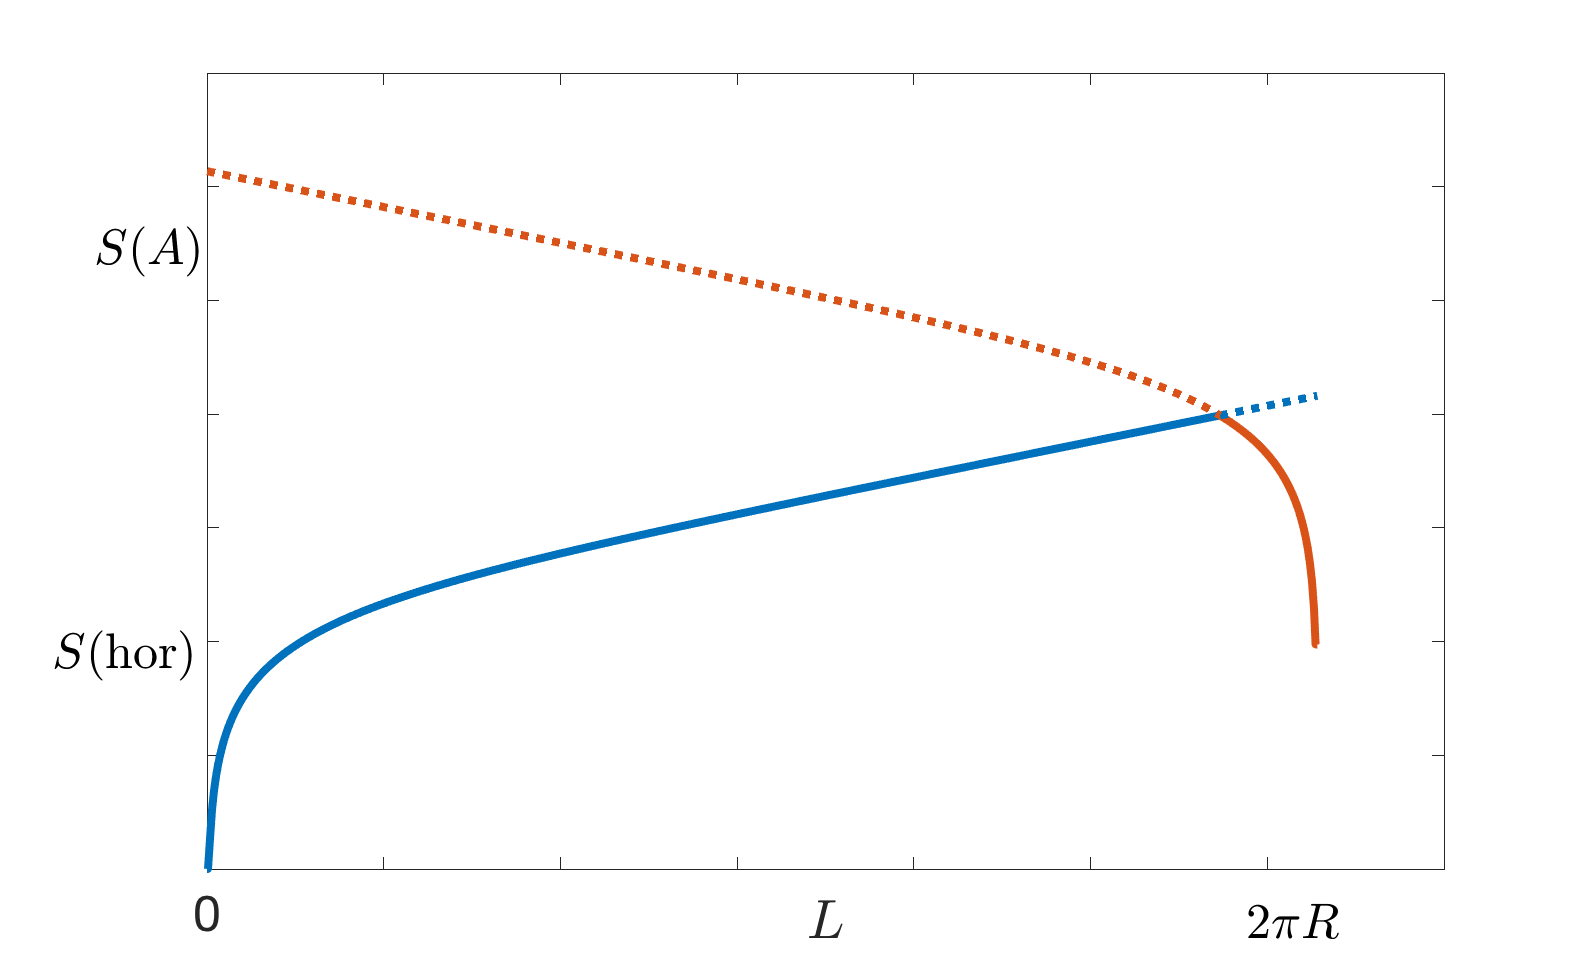
\includegraphics[width=0.65\textwidth]{figures/pagecurveplot0.png}
    \caption{The entropy of $A$ follows a sort of Page curve (\ref{BTZ interval entropy}). The minimal surface will switch from (\ref{length BTZ red}) to (\ref{length BTZ blue}) as $A$ becomes bigger. This resembles a phase transition.}
    \label{BTZ entropy phase transition}
\end{figure}



\addchap{Hawking Radiation, Entropy and Islands}
\setcounter{chapter}{3}
\refstepcounter{chapter}
\label{section 4}
In this chapter we review the thermodynamics of black holes as well as Hawking's information paradox. This paradox is solved by means of Quantum extremal surfaces (QES) \cite{almheiri2020entropy}.

\section{Black holes as thermal objects}

There were many hints indicating a relation between black holes and thermodynamics. For instance, the surface gravity $\kappa$ is constant over the event horizon of a stationary black hole. This motivates the zeroth law where, in thermodynamics, all parts of a system at thermodynamical equilibrium have equal temperature $T$. Also if one wants to study the behaviour of a QFT in a black hole spacetime, then the equilibrium of the system requires that the black hole has a temperature. This assigns a temperature to black holes and therefore they should be considered thermodynamical objects. And finally, we have an area theorem stating that the area of the event horizon is a non decreasing function of time. This suggests an analogy between black hole area $A$ and entropy $S$.

\subsection{First and second laws of thermodynamics}

In the 1970s, Bekenstein and others \cite{Bekenstein1972, PhysRevD.7.2333, PhysRevLett.25.1596} found equations that dictate black hole dynamics resembling those of thermodynamics,
\begin{equation}\label{1st law v1}
    \frac{\kappa}{8\pi G_N}\text{d}\left(\text{area}\right) = \text{d}M -\Omega\text{d}J + \phi\text{d}Q
\end{equation}
where $\kappa$ is the surface gravity, Area is that of its horizon, $M$ is its mass, $J$ the angular momentum, $\Omega$ is the rotational velocity of the horizon, $\phi$ the electric potential and $Q$ its charge. in this note, we are only interested in static neutral black holes where $J=0$ and $Q=0$.

If we postulate that the black hole entropy is proportional to the horizon area and has a temperature $\propto \kappa$, then (\ref{1st law v1}) looks exactly like the first law of thermodynamics
\begin{equation}\label{1st law v2}
    T\text{d}S_{\text{BH}} = \text{d}M -\Omega\text{d}J + \phi\text{d}Q.
\end{equation}
The reason why the entropy postulate makes sense, is that classically the area of the horizon is a non decreasing function of time. This resembles the second law of thermodynamics. The second law then reads\cite{Townsend:1997ku}: \begin{quote}
    If $T_{\mu\nu}$ satisfies the weak energy condition\footnote{The weak energy condition reads $v^\mu v^\nu T_{\mu\nu}\geq 0$ $\forall v$ non space-like. It is a condition that is used to constrain the solutions of Einstein field equations. It removes some solutions that are thought to be unphysical.}, and assuming that the cosmic censorship hypothesis\footnote{The cosmic censorship conjecture, proposed by Roger Penrose, states that there are no naked singularities, like a white hole, and therefore all singularities are hidden inside the event horizon. Up to this day, there is no rigorous proof of this conjecture. This is a major unsolved problem in classical G.R.} is true then the area of the future event horizon of an asymptotically flat spacetime is a non-decreasing function of time.
\end{quote}

This suggests that black holes are thermal objects. Indeed, Hawking discovered \cite{Hawking1975} that when coupled with quantum field theory, black holes have a temperature
\begin{equation}\label{Hawking temperature}
    T = \frac{\hbar \kappa}{2\pi}.
\end{equation}

If we consider the surrounding environment of a black hole, it could evaporate via Hawking radiations. Hawking radiation process can be interpreted as pair creation of entangled particles near the horizon, with one particle escaping to infinity and the other falling toward the singularity. Then the black hole slowly shrinks as its mass is carried away by the radiation. This would imply a decrease of the area in violation with the second law. We can solve this problem by assigning an entropy to the black hole as well as to the exterior. From (\ref{1st law v1}) and (\ref{Hawking temperature}), we find the total generalized entropy of a black hole to be
\begin{equation}\label{generalized entropy}
    S_{\text{gen}} = \frac{\text{Area}}{4\hbar G_N} + S_\text{outside},
\end{equation}
where $S_\text{outside}$ is the entropy of the QFT outside the horizon.

\section{Hawking information paradox}

Consider a black hole created from the collapse of a pure state. As time evolves, the black hole will emit thermal radiations. The origin of this thermal state is coming from entanglement as was discussed in the case of the thermofield double. As vacuum contains pairs of particles that are created and annihilated constantly, in the presence of a horizon things can be different. We can have one member of the entangled pair being absorbed by the horizon, while the other escapes it  and goes to infinity. This is the idea behind Hawking radiation \cite{Hawking1975}.

If we compute the entropy of radiations at early stages of evaporation, we will find it to be almost thermal as it is entangled with the quantum system and will start to increase as more Hawking quanta are emitted. However, as the black hole evaporates, its area becomes smaller and smaller, and therefore its thermal entropy (\ref{generalized entropy}) will decrease. As the black hole and the outside environment full of radiation, together, form a pure state, then by (\ref{Araki-Lieb}), $S_{\text{black hole}}=S_\text{rad}$. However, this fine-grained entropy cannot be bigger than the thermodynamic entropy (\ref{generalized entropy}), since it is not possible for the entropy of radiation to be entangled with a quantum system describing the black hole with fewer number of degrees of freedom (given by the thermodynamic entropy),
\begin{equation}
    S_{\text{black hole}}=S_\text{rad}\leq S_\text{Bekenstein-Hawking}.
\end{equation}

If the central dogma is to be true, then $S_\text{rad}$ should be expected to decrease once it becomes equal to $S_\text{Bekenstein-Hawking}$. The time at which this happens is called the Page time. The information paradox is summarized in figure \ref{Page curve}.

The Page time is achieved at an early stage compared to the Planck time $\sim 10^{-44}$s. So it should be possible to resolve this paradox in a semi-classical approximation.

\begin{figure}
    \centering
    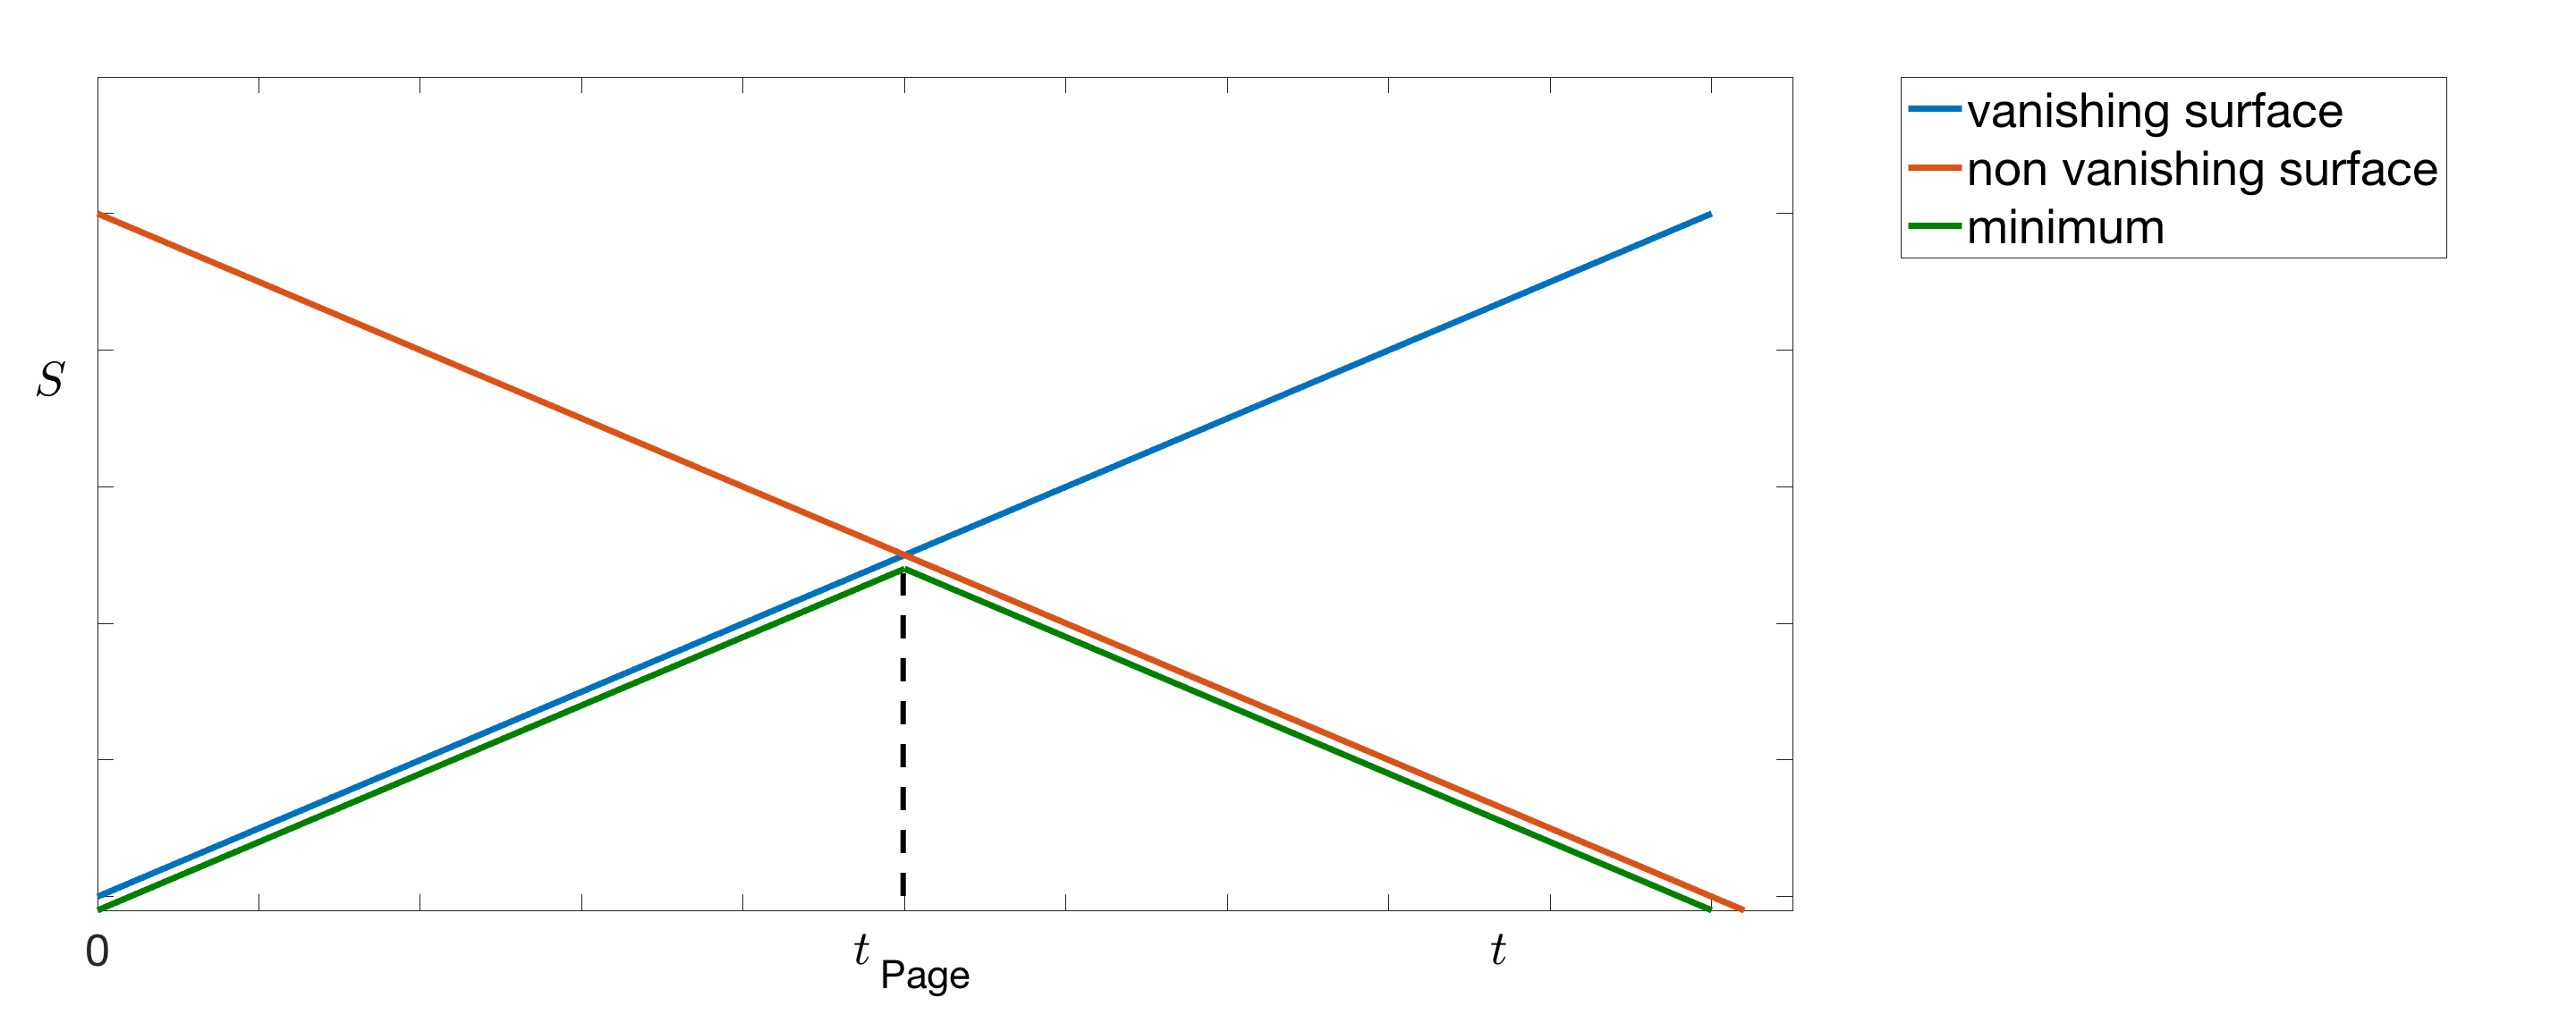
\includegraphics[width=0.8\textwidth]{figures/page_island.png}
    \caption{Behaviour of radiation entropy during black hole evaporation. The increasing green curve is what was originally computed by Hawking. The decreasing orange curve is the thermodynamic entropy of the black hole. The Page curve in blue is the expected entropy in case we consider the central dogma hypothesis.}
    \label{Page curve}
\end{figure}

\section{Entropy of an evaporating black hole}

The central dogma considers the black hole and its surrounding region delimited by a cutoff surface to be equivalently described by a quantum system with large, but finite, degrees of freedom. The gravitational formula for the black hole von Neumann entropy is computed by minimizing (\ref{generalized entropy}) with respect to this cutoff surface
\begin{equation}\label{approx gravitational fine grained}
    S \sim \text{min}\left[\frac{\text{Area}}{4\hbar G_\text{N}} + S_\text{outside}\right].
\end{equation}

The actual formula is more than that. One equivalent definition is to take a Cauchy slice and find a minimal surface. Then choose the Cauchy slice that gives the maximum. The fine-grained entropy is then
\begin{equation}\label{gravitational fine grained}
    S = \min_X\left\{\text{ext}_X\left[\frac{\text{Area}\left(X\right)}{4\hbar G_\text{N}} + S_\text{semi-cl}\left(\Sigma_X\right)\right]\right\}.
\end{equation}
where $X$ is a codimension 2 surface called the quantum extremal surface (QES) and $\Sigma_X$ the slice on its left bounded by the cutoff surface as shown in fig. \ref{evaporation bh}.

When computing the fine grained entropy of the black hole using eq (\ref{gravitational fine grained}), we find two extremal quantum surfaces. The first case is the one with a vanishing surface. This contribution gives an increasing entropy as a function of time. The other extremal surface appears right after outgoing Hawking quanta escape the black hole. It lies close to the horizon. The generalized entropy now has a non vanishing area and the von Neumann entropy of the exterior quantum fields can be neglected. This entropy follows almost the shape of the thermodynamic entropy,
\begin{equation}
    S = \frac{\text{Area}_\text{hor}\left(t\right)}{4\hbar G_\text{N}}.
\end{equation}
Since (\ref{gravitational fine grained}) requires to take the minimum, we end up having an increasing entropy coming from the vanishing QES, and a decreasing entropy given by non vanishing QES. The overall shape of the curve follows the Page curve. The Page time is when the two extremal surfaces cross.

\begin{figure}
    \centering
    \begin{subfigure}[b]{0.3\textwidth}
        \centering
        \begin{tikzpicture}\label{evaporating bh}
            \draw (0,3) -- (0,-2.5)
            -- (5,2.5) -- (3,4.5)
            [sharp corners] -- (3,3);
            \draw [densely dotted] (0,0) -- (3,3);
           
            \fill[yellow, draw=black] (0,-2.5) .. controls (0.5,0.5) .. (0,3);
           
            \draw[densely dotted,color=blue] (0,-2.5) .. controls (3.5,3) .. (3,4.5);
           
            \draw[color=green] (0.5,1) parabola (2.5,1.5);
           
            \filldraw[green] (0.5,1) circle (2pt) node[anchor=west] {~~~~~~~~~~~$\Sigma_X$};
            \node[above right=.5pt of {(.5,1)}, outer sep=2pt, color=green] {$X$};
           \draw[decorate,decoration=zigzag] (0,3)
           -- (3,3);
        \end{tikzpicture}
        \caption{}
        \label{evaporation bh}
    \end{subfigure}
    \hfill
    \begin{subfigure}[b]{0.3\textwidth}
        \centering
        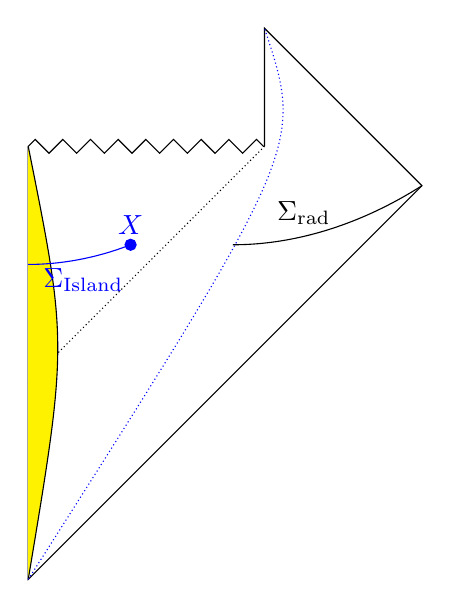
\begin{tikzpicture}
            \draw (0,3) -- (0,-2.5)
            -- (5,2.5) -- (3,4.5)
            [sharp corners] -- (3,3);
            \draw [densely dotted] (0,0) -- (3,3);
           
            \fill[yellow, draw=black] (0,-2.5) .. controls (0.5,0.5) .. (0,3);
           
            \draw[densely dotted,color=blue] (0,-2.5) .. controls (3.5,3) .. (3,4.5);
            \draw (2.6,1.75) parabola (5,2.5);
            \draw[color=blue] (0,1.5) parabola (1.3,1.75);
            
            \filldraw[blue] (1.3,1.75) circle (2pt) node[anchor=south] {$X$};
            \draw[blue] node at (.7,1.3){$\Sigma_\text{Island}$};
           \draw[decorate,decoration=zigzag] (0,3)
           -- (3,3);
           %\draw[->]   (3.5,1.8) -- + (1,-1);
           %\draw[blue] node at (4.5,.6){$\Sigma_\text{rad}$};
           \draw node at (3.5,2.15){$\Sigma_\text{rad}$};
        \end{tikzpicture}
        \caption{}
        \label{evaporation rad}
    \end{subfigure}
    \caption{Penrose diagram of an evaporating black hole. The black hole is considered to be formed from the collapse of a pure state. (a) The quantum extremal surface for computing the fine grained entropy of the black hole. (b) The quantum extremal surface for computing the fine grained entropy of radiation. In this case we have a possible contribution coming from inside the horizon (the Island) which results in the decrease of the entropy.}
    \label{island radiation}
\end{figure}


This does not solve the Hawking information paradox yet, since it involves the entropy of radiations. However, we can use the same formula (\ref{gravitational fine grained}) to compute radiation entropy. There is no reason why $\Sigma_X$ cannot be disconnected. Indeed that is exactly the case for Hawking radiations. Computations through gravitational path integral suggest to include the interior for the black hole as well \cite{Marolf_2021}. This interior region behind the horizon that is included in the computation of radiation entropy is called an island. The fine grained entropy becomes
\begin{equation}\label{rad fine grained}
    S = \text{min}_X\left\{\text{ext}_X\left[\frac{\text{Area}\left(X\right)}{4\hbar G_N} + S_\text{semi-cl}\left(\Sigma_\text{Rad}\cup\Sigma_\text{Island}\right)\right]\right\}
\end{equation}
where the area is the boundary of the Island, figure \ref{island radiation}.

The straightforward possibility is the case with no island. In this case radiation entropy just increases as computed by Hawking. After some time, of order $r_s\log S_{BH}$, a non-vanishing island that extremises (\ref{rad fine grained}) appears. Since the von Neumann entropy includes the region inside the black hole, the entropy decreases over time. This is due to the interior Hawking quanta purifying the exterior modes\footnote{A very good analogy was given at the end of section 8 of \cite{almheiri2020entropy}.}. The minimum of the two extremums follows exactly the Page curve.


\addchap{Holographic Interface CFT}
\setcounter{chapter}{4}
\refstepcounter{chapter}
\label{section 5}
In this section we are going to describe the system that we are going to work on (the system for which we want to compute RT surfaces) which features interface CFTs. We start by summarizing results of \cite{Bachas_2021}, where two CFTs were considered separated by an interface. The dual geometry features a domain wall separating two classical geometries which could be part of thermal AdS or BTZ black hole geometry. Since the general system can be in numerous phases, we prefer to consider only one phase. We take the limit of some large canonical variables and Lagrangian parameters to determine the dominant phase in that case. We use the same notations as \cite{Bachas_2021}.

\section{The general system}\label{general system}

We consider two conformal field theories, CFT$_1$ and CFT$_2$, on a circle at thermal equilibrium $T$. The two CFTs are characterized by their central charges, $c_1$ and $c_2$ respectively, and are separated by an interface characterised by its tension $\lambda$. In addition to that, there are two additional parameters, and these are the sizes of the regions occupied by the two CFTs: $L_1$ and $L_2$. We refer to the side with size $L_1$ as the red slice and the one with size $L_2$ as the blue slice as in fig. \ref{ICFT}.

\begin{figure}[h!]
    \centering
    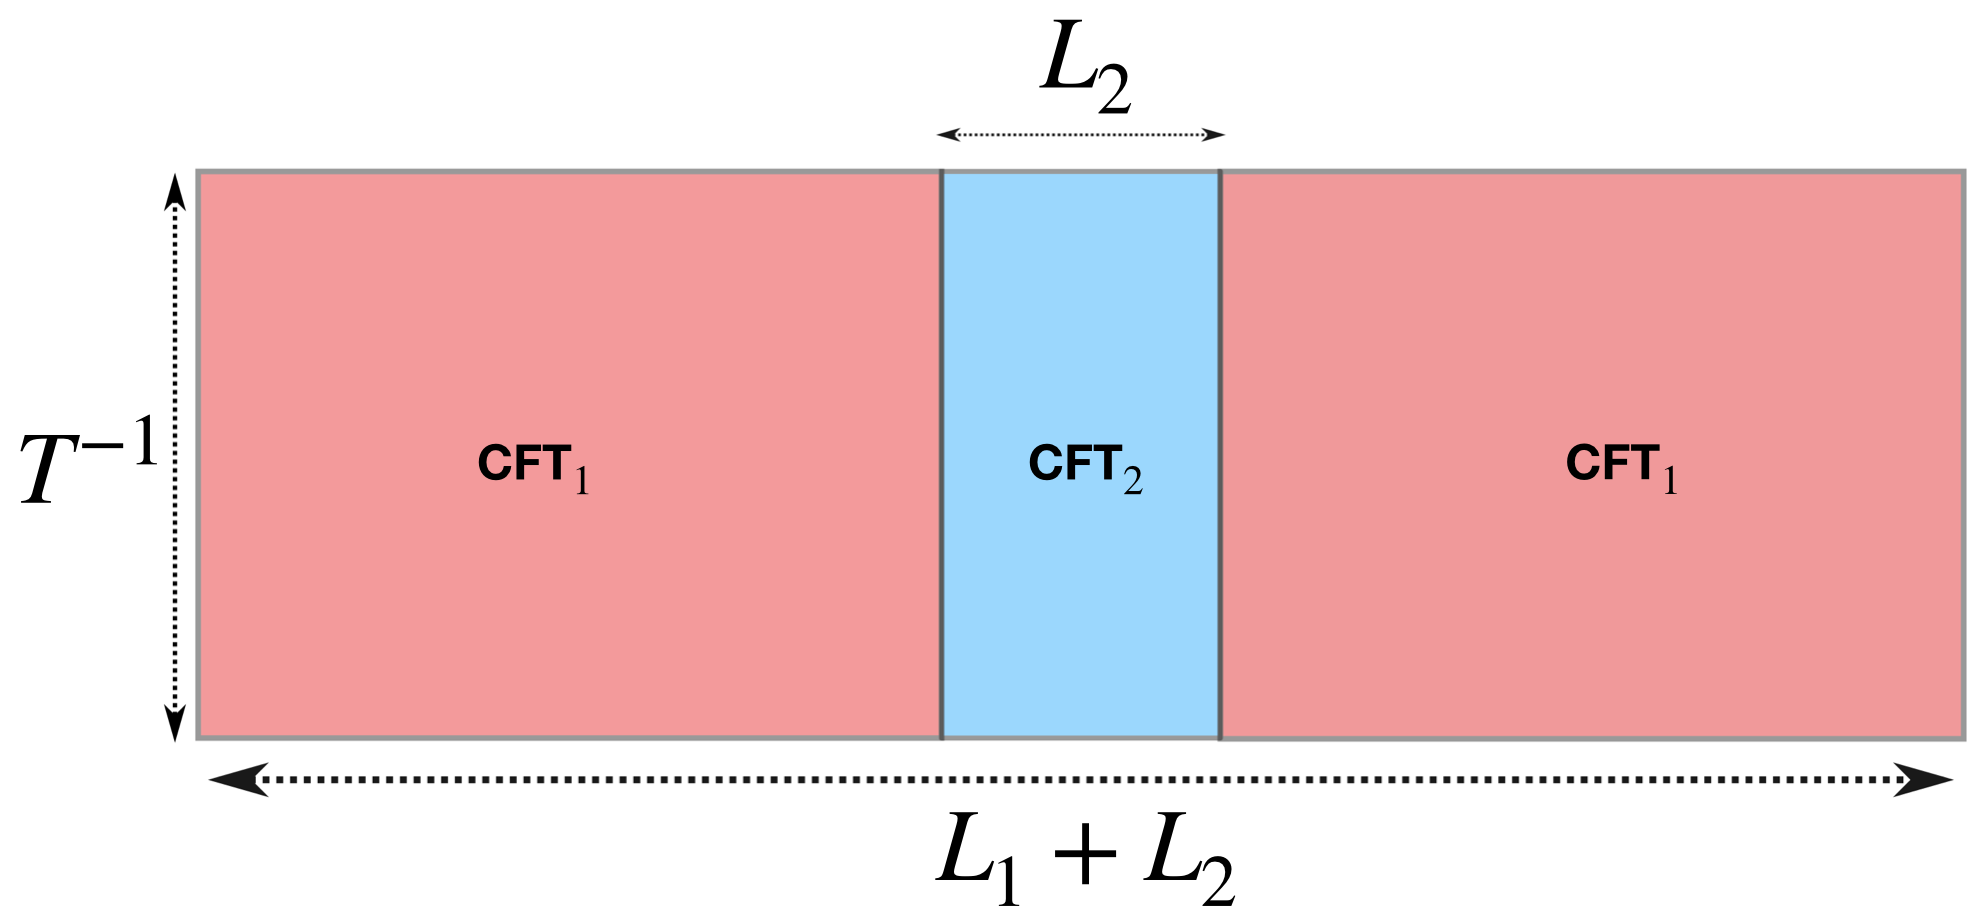
\includegraphics[width=0.65\textwidth]{figures/ICFTb.png}
    \caption{AdS boundary with 2 CFTs separated by an interface. Space and Euclidean time are compact. The red region was intentionally made larger than the blue one as we will tend to consider the case $L_1\gg L_2$ lately.}
    \label{ICFT}
\end{figure}

The two regions extend in the interior to gravitational solutions with different topologies, separated by a domain wall. The action is that given in (\ref{action cft}). The AdS radii $\ell_i$ are related to the central charges via $c_i = 12\pi\ell_i$. We work in Planck units where $8\pi G = 1$.

The boundary is extended in the interior into gravitational solutions of two types: thermal AdS or BTZ black hole. The two slices can be parts of these solutions, having several topologies as presented in fig. \ref{topologies}. The solution could be part of thermal AdS$_3$, either with a center $($E$1)$ or centerless $($E$2)$, or could be part of a BTZ black hole, either with a complete horizon $($H$1)$ or a part of it $($H$2)$ or horizonless $($E$2')$.

\begin{figure}
    \centering
    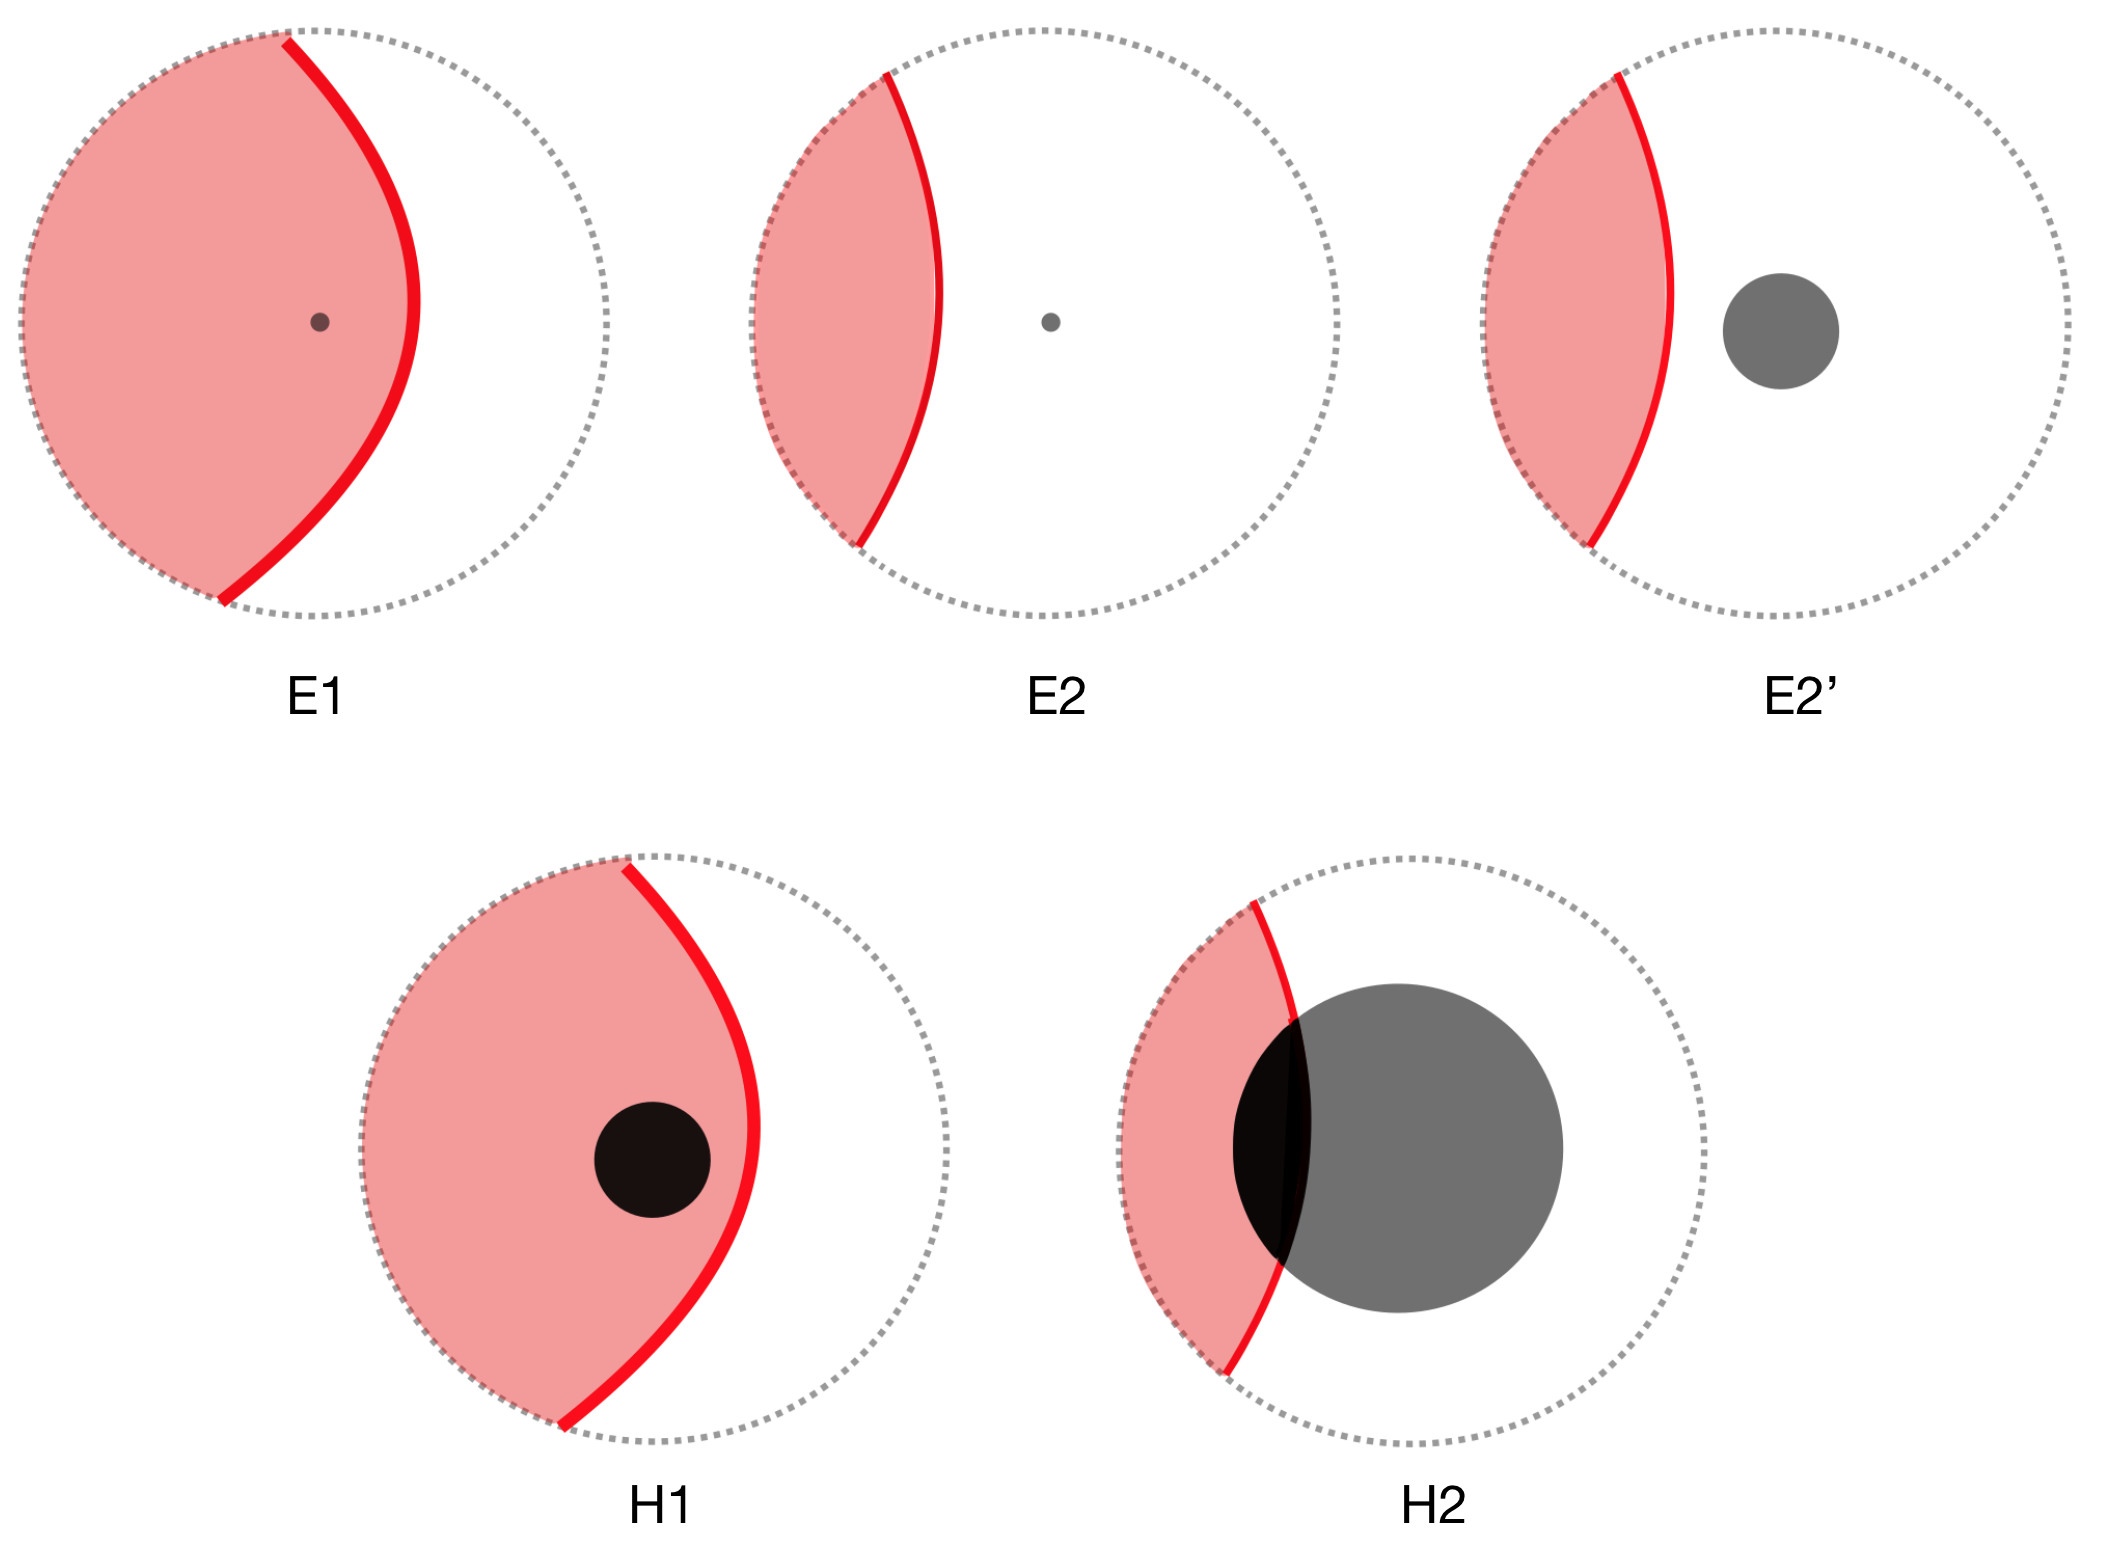
\includegraphics[width=0.65\textwidth]{figures/phasesred.png}
    \caption{Different topologies depending on the geometry (thermal AdS or BTZ) and the wall. We represent the solutions for the red slice, while the blue slice is supposed to have the same solutions.}
    \label{topologies}
\end{figure}

We write the metric in terms of two coordinate charts $\left(x_j,r_j\right)$ and the globally defined time $t$:
\begin{equation}\label{geometry}
    \text{d}s^2 = \frac{\ell_j^2}{r_j^2-M_j\ell_j^2}\text{d}r_j^2 - \left(r_j^2-M_j\ell_j^2\right)\text{d}t^2+r_j^2\text{d}x_j^2
\end{equation}
with $\left(x_j,r_j\right)\in \Omega_j$, where $\Omega_j$ is the range of coordinates in each slice, determined by the wall, the horizon (when it exists) and the cutoff surface $r_j\sim 1/\epsilon$.

There are two important points to notice. The first one is that regularity requires that for H$1$ and H$2$ slices we have $M_j=\left(2\pi T\right)^2$. The second point is that there is no topological difference between E$2$ and E$2'$. These two solutions differ only by the sign of the mass $M_j$.

A change of coordinates that will be used later is,
\begin{align}\label{change of coord rz}
    r_j=\frac{1}{z_j},         &&           t=T_j\ell_j,          &&        x_j=\phi_j\ell_j.
\end{align}

In these new coordinates the metric (\ref{geometry}) takes the form
\begin{equation}\label{geometry z}
    \text{d}s^2 = \frac{\ell_j^2}{z_j^2}\left(\frac{1}{f_j(z_j)}\text{d}r_j^2 - f_j(z_j)\text{d}T_j^2+\text{d}\phi_j^2\right),
\end{equation}
where $f_j(z_j)=1-\frac{z^2}{{z_j}_h^2}$ and ${z_j}_h=\frac{1}{\ell_j\sqrt{M_j}}$.

\section{The wall equation}

\subsection{Determining the range of $\lambda$}

The different parameters of our system, the mass parameters $M_j$, the AdS radii $\ell_j$, and the tension of the wall $\lambda$, must obey different equations. A set of these equations are the matching conditions. They guarantee that there is a well defined metric on the wall. These are given by matching the metric of the two slices at the wall as was presented in \cite{Simidzija_2020,Bachas_2021}:
\begin{align}
    &r_j^2-M_j\ell_j^2=f(\sigma) \label{matching condition 1} \\
    f&^{-1}\ell_1^2r'_j^2 + r_j^2x'_j^2 = g(\sigma) \label{matching condition 2}
\end{align}
where the prime corresponds to a derivative with respect to $\sigma$ the wall parameter. The two functions $f(\sigma)$ and $g(\sigma)$ are the diagonal terms of the wall induced metric, $\text{d}\hat{s}^2=-f(\sigma)\text{d}t^2+g(\sigma)\text{d}\sigma^2$. The other matching condition, known as the Israel-Lanczos\cite{Israel:1966rt} matching condition, can be written as:
\begin{equation}\label{Israel-lanczos}
    \frac{r_1^2x'_1}{\ell_1} +  \frac{r_2^2x'_2}{\ell_2} = \lambda\sqrt{fg}.
\end{equation}

Solving (\ref{matching condition 1}), (\ref{matching condition 2}) and (\ref{Israel-lanczos}) near the boundary, where $M_j$ can be neglected, is not complicated. The solution gives the possible values of $\lambda$ for a static solution. We find that $\lambda$ has a minimum and a maximum value:
\begin{equation}\label{domain wall}
    \lambda_{\text{min}} <\lambda< \lambda_{\text{max}},
\end{equation}
where the critical tensions  are,
\begin{align}
     \lambda_{\text{min}} = \frac{1}{\ell_1} - \frac{1}{\ell_2} &&  \lambda_{\text{max}} = \frac{1}{\ell_1} + \frac{1}{\ell_2}.
\end{align}
The complete derivation can be found in \cite{Bachas_2021}, section 4.

\subsection{General solutions}\label{solutions}

The general solutions of (\ref{matching condition 1}), (\ref{matching condition 2}) and (\ref{Israel-lanczos}) are found by considering a convenient parametrization of the wall outside the horizon, see \cite{Bachas_2021}. The solutions are the following:
\begin{subequations}
\label{wall solution}
\begin{align}
     r_j &= \sqrt{|\sigma| + M_j\ell_j^2},\label{solution r} \\
     \frac{x'_1}{\ell_1} &= -\frac{\sigma\left(\lambda^2+{\lambda_0}^2\right)+M_1-M_2}{2\left(\sigma+M_1{\ell_1}^2\right)\sqrt{A\sigma\left(\sigma-\sigma_+\right)\left(\sigma-\sigma_-\right)}},\label{solution x1} \\
     \frac{x'_2}{\ell_2} &= -\frac{\sigma\left(\lambda^2-{\lambda_0}^2\right)+M_2-M_1}{2\left(\sigma+M_2{\ell_2}^2\right)\sqrt{A\sigma\left(\sigma-\sigma_+\right)\left(\sigma-\sigma_-\right)}}, \label{solution x2}
\end{align}
\end{subequations}
where $A = \left({\lambda_\text{max}}^2-{\lambda}^2\right)\left(\lambda^2-{\lambda_\text{min}}^2\right)$ and $\sigma_\pm$ are poles of $g(\sigma)$.

The above equations give solutions of the wall equation in terms of the mass parameters $M_j$. These parameters are not free to choose. They must obey the Dirichelet boundary conditions:
\begin{gather}\label{Dirichelet bc}
    L_j = 2{\int_{\sigma_+}}^\infty \text{d}\sigma\,x'_j \quad \text{for     E2, E2}'; \\
    L_j = nP_j + 2{\int_{\sigma_+}}^\infty \text{d}\sigma\,x'_j \quad \text{for     E1, H1;} \\
    L_j = \Delta x_j|_\text{Hor} + 2{\int_{\sigma_+}}^\infty \text{d}\sigma\, x'_j \quad \text{for     H2.}\label{Dirichelet hot}
\end{gather}
where $P_j$ is the period of $x_j$, $n$ the winding number and $\Delta x_j|_\text{Hor}$ is Horizon arc in the $j$th slice

\section{Allowed phases}\label{tablesec}

From the different topologies described in section \ref{general system}, only some of theme can be paired together. These are results of three no-go lemmas\footnote{See section 5 of \cite{Bachas_2021}.}. The possible phases are described in fig. \ref{table}.

\begin{figure}
    \centering
    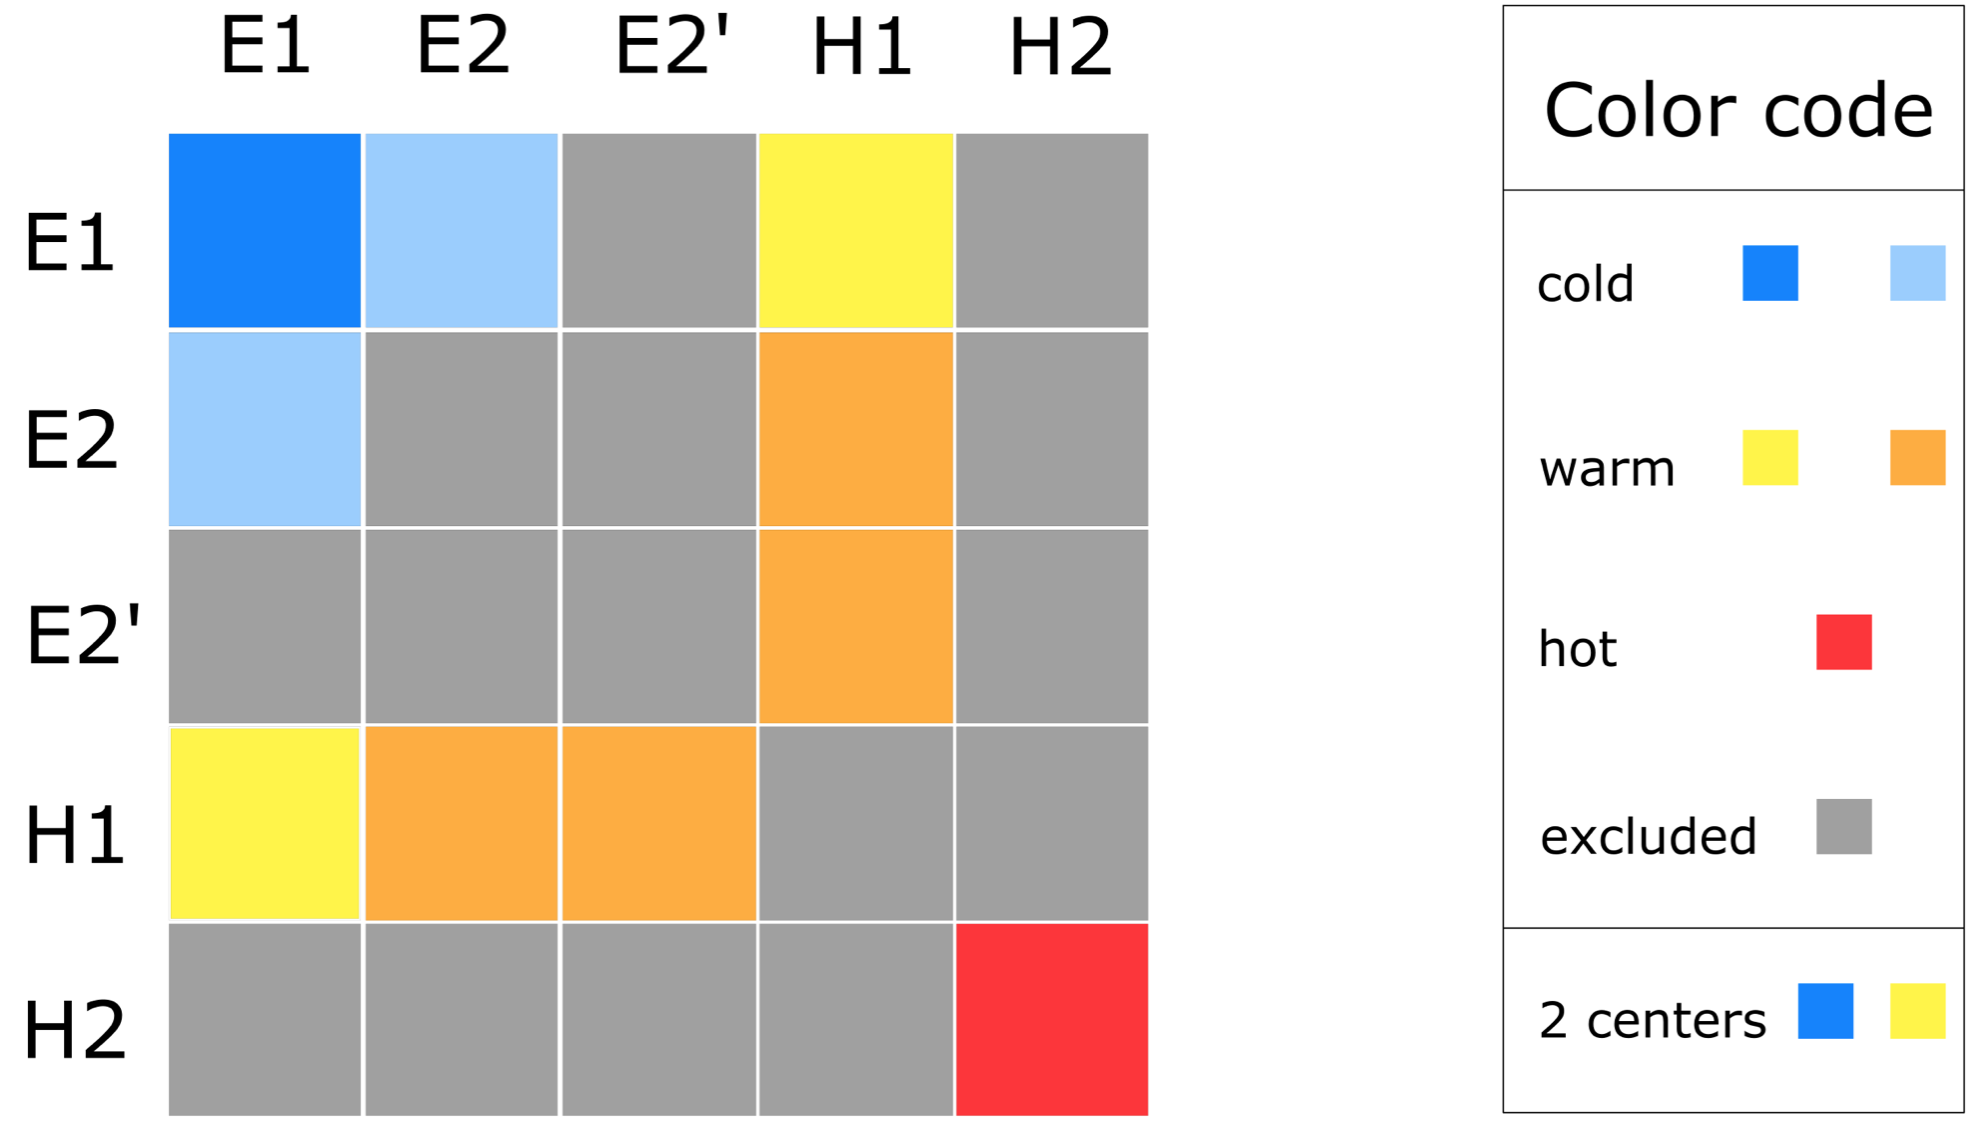
\includegraphics[width=0.65\textwidth]{figures/table.png}
    \caption{Phases of the domain-wall spacetime. The type of the red slice labels the rows of the table, and that of the blue slice the columns.}
    \label{table}
\end{figure}

We use the notation $[$X$_1$,X$_2]$ to describe a solution with X$_1$ topology in the red side and X$_2$ topology in the blue slice. Note that two of the allowed phases are double centered, one is cold $\left[\text{E}1,\text{E}1\right]$ and the other one is the warm one $\left[\text{E}1,\text{H}1\right]$. 

Another point to mention is that horizons are more likely to form in the true vacuum, i.e the slice with the smallest ground state energy. This energy can be computed by means of the stress energy tensor and is found to be an increasing function of the central charge,
\begin{equation}
    E_0 \propto -\frac{1}{c^2}.
\end{equation}
In \cite{Bachas_2021}, it was shown numerically that solutions with horizons on the false vacuum side cease to exist as we surpass the the critical value $b=\frac{\ell_2}{\ell_1}=3$.

\section{The limit of Large $L_1$ and $\ell_2$}\label{limit}

We want to create a system where a part of it is characterised with a large number of degrees of freedom, coupled to a very large region modeling a bath. We take the limit of large central charge for the blue slice $\ell_1\ll \ell_2$, and large boundary region for the red slice $L_1\gg L_2$. We also consider $\lambda\rightarrow\lambda_{\text{min}}$ so the wall can be as transparent as possible. We want to find which of the phases described in the previous section is the dominant one in this limit.

In order to determine the dominant phase, we think thermodynamics, where we have fixed Lagrangian parameters $\lambda$ and $\ell_j$, and canonical variables that determine the state, $T$ and $L_j$. Because of scale invariance, we work with four dimensionless parameters,
\begin{align}
    \tau_j:=TL_j, && \gamma:= \frac{L_1}{L_2}, && \text{and} \quad \mu := \frac{M_2}{M_1}.
\end{align}

The energy and Entropy of each subsystem is given by
\begin{equation}
    E_j = \frac{L_j\ell_j}{2}M_j \quad \text{and} \quad S_j = 2\pi\ell_j\sqrt{M_j}\Delta x_j|\text{Hor}.
\end{equation}

The dominant phase is the one that has the lowest free energy,
\begin{equation}
    F = \sum_j E_j -T S_j.
\end{equation}

The free energy can be computed in terms of $\tau$, using the boundary conditions (\ref{Dirichelet bc}).

\subsection{Possible solutions}

In the limit we are working on, we have $\gamma,\tau \gg 1$. In this case we can already rule out cold solutions of type $\left[\text{E}1,\text{E}1\right]$, $\left[\text{E}1,\text{E}2\right]$ and $\left[\text{E}2,\text{E}1\right]$.
 
We are left with the warm and hot solutions. These are $\left[\text{H}1,\text{E}1\right]$, $\left[\text{H}1,\text{E}2\right]$, $\left[\text{H}1,\text{E}2'\right]$ and $\left[\text{H}2,\text{H}2\right]$. As we have mentioned in the end of section \ref{tablesec}, we have ruled out the solutions with H1 on the blue side since the red side is the true vacuum, $\ell_1\ll\ell_2$.
 
We can also rule out $\left[\text{H}1,\text{E}1\right]$. The difference between E$1$ (with a center) and E$2$ (centerless) is the sign of $x_2'$ at the turning point $\sigma_+$, which is
\begin{equation}
    \text{sign}(x_2')|_{\sigma_+} = 
    \left\{
    \begin{array}{lll}
        -1 & \mbox{if} & X_2=\text{E}1, \\
        +1 & \mbox{if} & X_2=\text{E}2.
    \end{array}
\right.
\end{equation}

If we consider the case of light walls $\lambda\rightarrow\lambda_{\text{min}}$ and since $X_1=$H$1$, we can see from (\ref{solution x2}) that $x_2'(\sigma)>0$ at $\sigma_+$. We are therefore in the case $X_2=$E$2$. The condition $\lambda<\lambda_0$ is sufficient.

\subsection{The free energy}

In order to determinant the dominant phase of the rest of the allowed phases, we have to compare their free energies. The general form of the free energy was already introduced in section \ref{limit}. The three free energies that we are interested in have the same divergent term (the term proportional to $L_1$). This part can be omitted.

The expression of the free energies are then:
\begin{subequations}\label{free E}
    \begin{align}
        \Tilde{F}\left(\left[\text{H}1,\text{E}2\right]\right) &=\frac{\ell_2}{L_2}\left( \frac{1}{2}\mu\left(\tau_2\right)\left(2\pi\tau_2\right)^2 - \frac{2\pi}{{b}}\Tilde{f}_1(\tau_2)\tau_2\right), \label{F(E2)}\\
        \Tilde{F}\left(\left[\text{H}1,\text{E}2'\right]\right) &=\frac{\ell_2}{L_2}\left( \frac{1}{2}\mu\left(\tau_2\right)\left(2\pi\tau_2\right)^2 - \frac{2\pi}{{b}}\Tilde{f}_1(\tau_2)\tau_2\right), \label{F(E2')}\\
        \Tilde{F}\left(\left[\text{H}2,\text{H}2\right]\right) &=\frac{\ell_2}{L_2}\left( -\frac{1}{2}\left(2\pi\tau_2\right)^2 - (2\pi)^2\left(\frac{g_1\left(\lambda\right)}{b}+g_2\left(\lambda\right)\right)\tau_2\right). \label{F(H2)}
    \end{align}
\end{subequations}
$b$ is the ratio of the two central charges $b=\ell_2/\ell_1$. The difference between $\Tilde{F}\left(\left[\text{H}1,\text{E}2\right]\right)$ and $\Tilde{F}\left(\left[\text{H}1,\text{E}2\right]\right)$ lies in the sign of $\mu$ which is negative for (\ref{F(E2)}) and positive, yet smaller than 1, for (\ref{F(E2')}). By $\Tilde{F}$ we mean "$F-\text{divergent part}$", which is 
\begin{equation}
    \Tilde{F} = F + \frac{\ell_1L_1}{2}(2\pi T)^2.
\end{equation}

Note that $\mu$, the ratio of the two masses, depends on $\tau_2$ through $f_2$, while it is equal to 1 in the hot phase. The functions $\Tilde{f}_i$ are rewritten versions of the boundary conditions (\ref{Dirichelet bc}). The full derivation of their expression is detailed in appendix \ref{appendix D}.
\begin{align}\label{f2 constrain}
     2\pi T\Delta\big|_\text{Hor} -2\pi\tau_1= \Tilde{f}_1(\mu), && 2\pi\tau_2= -\Tilde{f}_2(\mu).
\end{align}

The function $\Tilde{f}_2(\mu)$ can be expressed in terms of the Elliptic integrals of the first, second and third kind,
\begin{equation}
    \Tilde{f}_2(\mu) = \frac{2\ell_2}{\sqrt{As_+}}\left[\frac{1-\mu}{s_+ u}\left(\bm{K}(\nu)-\bm{\Pi}(u,\nu)\right)+\left(\lambda^2-\lambda_0^2\right)\bm{\Pi}(u,\nu)\right],
\end{equation}
where $s_\pm=\sigma_\pm/M_1$, $\nu=s_-/s_+s$ and $u=-\mu\ell_2^2/s_+$. The limit of $\Tilde{f_2}$ when $\mu\rightarrow0$ is well defined,
\begin{equation}
    \Tilde{f}_2(\mu=0) = \frac{2\ell_2}{\sqrt{As_+}}\left[\frac{1}{s_-}\left(\bm{E}(\nu)-\bm{K}(\nu)\right)+\left(\lambda^2-\lambda_0^2\right)\bm{K}(\nu)\right].
\end{equation}

The variable $\nu$ takes values in $(-\infty,0)$ and therefore the Elliptic integrals of the first and second kind are well behaved. The $\bm{\Pi}(u,\nu)$ integral diverges for $u=1$. This is the case when the string turning point and the the AdS center coincide $\sigma_+ = -M_2\ell_2^2$. This point specifies a sweeping transition between a center-less topology E2 and a center-full topology E1. This equation has one solution,
\begin{equation}\label{sweeping trans}
    \mu^* = \frac{1/b^2}{1-\ell_1^2\lambda}.
\end{equation}
Since both topologies E1 and E2 belong to part of thermal AdS geometry while the red side is fixed at H1, this sweeping transition between E1 and E2 happens at negative value of $\mu$. A sufficient condition to avoid this solution (\ref{sweeping trans}) is to take $\lambda\in(\lambda_\text{min},1/\ell_1))$. In this case $\mu^*>0$ and therefore the value $u=1$ is avoided.

Note that the function $\Tilde{f}_2(\mu)$ converges to 0 when $\mu\rightarrow-\infty$. This can be seen just by computing the limit of $s_+(\mu)\rightarrow\infty$. In conclusion, $\Tilde{f}_2$ is a negative finite function of $\mu$. As seen from equation (\ref{f2 constrain}), this function constrains the values of $\tau_2$ in the case of warm phases with centerless blue slices. As it takes only values in $(0,-\min\{\Tilde{f}_2\})$, the warm solutions will cease to exist for high $\tau_2$, i.e high $T$.

The hot phase $\left[\text{H}2,\text{H}2\right]$ is constrained by the existence of the horizon on both sides, i.e $\Delta x_j|_{Hor}\geq0$. Solving this inequality, we get a lower bound for $\tau_2$,
\begin{equation}
    \tau_2\geq\frac{1}{\pi}\tanh^{-1}\left(\frac{\ell_2(\lambda_0^2-\lambda^2)}{2\lambda_0}\right):=\tau_2^*.
\end{equation}
The hot solution will exist for any temperature higher than $\tau_2^*$ and therefore will be the only existing solution for $\tau_2\geq\max\left\{\tau_2^*,-\min\{\Tilde{f}_2\}\right\}$. This could be seen as analogous to a Hawking-Page transition where we take the temperature to be higher than some critical value in order to have a dominant solution in which a horizon exists in the blue slice.

\subsection{Example}

\begin{figure}
    \centering
    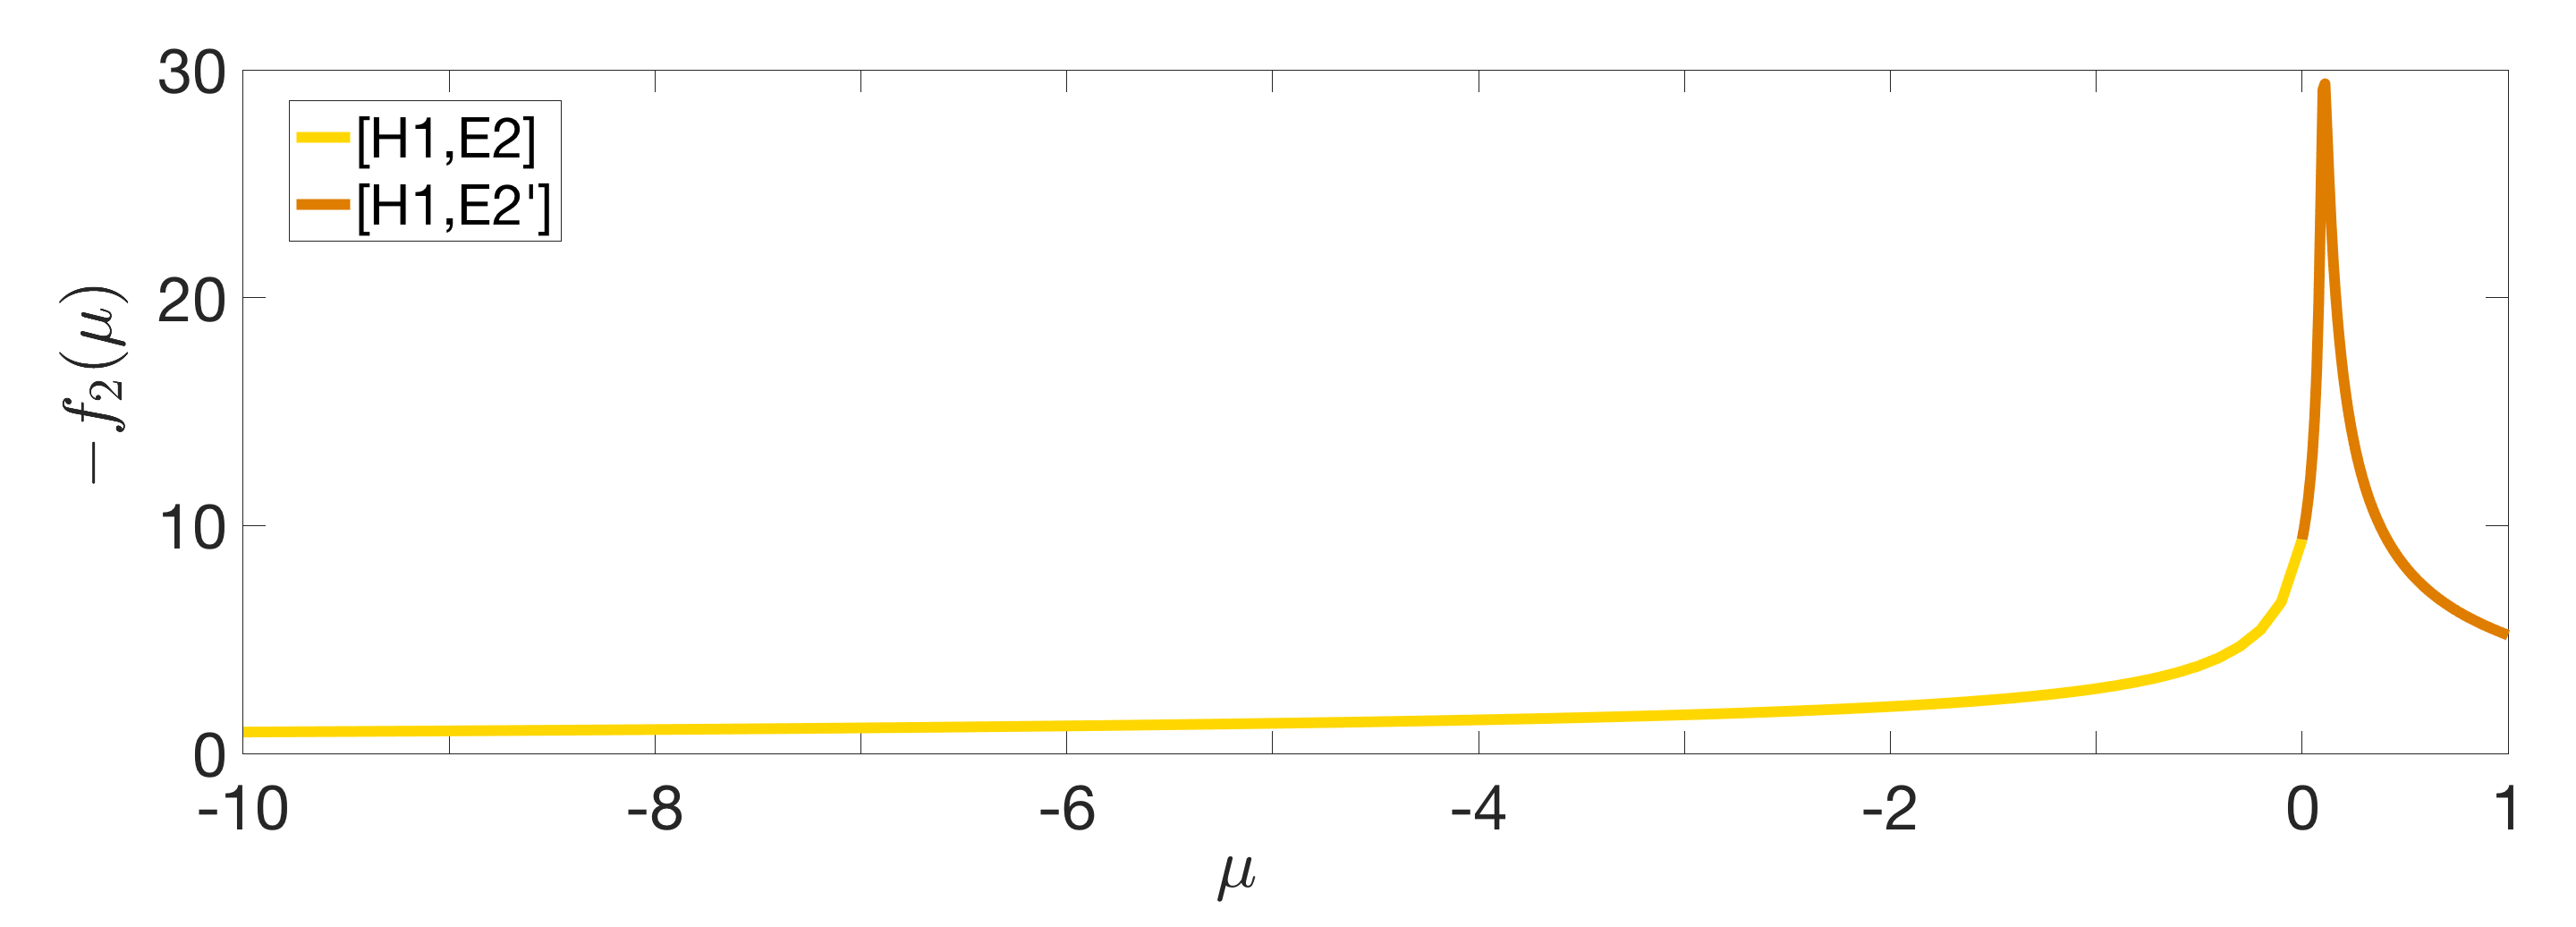
\includegraphics[width=0.9\textwidth]{figures/f2.png}
    \caption{The function $-\Tilde{f}_2(\mu)$ which determines $\tau_2$ through eq. (\ref{f2 constrain}). The point $\mu = 0$ represents the limit between the two warm phases. The function $\Tilde{f}_2(\mu)$ goes to zero for $\mu\rightarrow-\infty$.}
    \label{f2}
\end{figure}

Let's consider a special case and choose some values of $\ell_1$ and $\ell_2$. We choose,
\begin{align}
    \ell_1 = 1, && \ell_2 = 10 && \text{and} && \lambda = \lambda_{\text{min}} + \frac{1}{100\ell_2}.
\end{align}

We plot $\Tilde{f}_2$ as a function of $\mu$ in fig. \ref{f2} with $\mu$ ranging from $-\infty$ to $1$. We see that the function $\Tilde{f}_2$ is negative as discussed before and has a minimum value at $\mu = \Tilde{\mu}>0$. From the shape that $\Tilde{f}_2(\mu)$ takes, we can determine some ranges of $\tau_2$ where warm phases can exist.

The function $\Tilde{f}_2$ for positive $\mu$ takes values between $\min\left\{\Tilde{f}_2(\mu)\right\}=\Tilde{f}_2(\Tilde{\mu})$ and $\max\left\{\Tilde{f}_2(\mu)\right\} = \Tilde{f}_2(1)$. This constrains the values of $\tau_2$ under which the phase $\left[\text{H}1,\text{E}2^{\prime}\right]$ can exist,
\begin{equation}
    -\Tilde{f}_2(1)\leq 2\pi\tau_2\leq - \Tilde{f}_2(\Tilde{\mu}).
\end{equation}

On the $\mu\leq 0$ side of the plot \ref{f2}, the function $-\Tilde{f}_2(\mu)$ is only increasing, having its minimum 0 when $\mu\rightarrow-\infty$ and its maximum at $-\Tilde{f}_2(0)$. Therefore, the warm phase $\left[\text{H}1,\text{E}2\right]$ exists for
\begin{equation}
    0 \leq 2\pi\tau_2\leq - \Tilde{f}_2(0).
\end{equation}

So in summary, we have a region where only $\left[\text{H}1,\text{E}2^\prime\right]$ exists, another region where only $\left[\text{H}1,\text{E}2\right]$ exists, and in between them a region where the two phases coexist. The hot phase on the other hand only exists for $\tau_2\geq\tau_2^*$. Note that when we say only a warm phase exists, we don't exclude the existence of the hot phase nor the cold phases. The results are summarized in table \ref{summary}.
\begin{table}
    \centering
    \begin{tabular}{ |c|c|c|c| } 
        \hline
        $2\pi\tau_2$ & 0 $\rightarrow -\Tilde{f}_2(1)$ & $-\Tilde{f}_2(1) \rightarrow -\Tilde{f}_2(0)$ &  $-\Tilde{f}_2(0) \rightarrow \Tilde{f}_2(\Tilde{\mu})$\\ 
        & & & \\
        \text{Phases} & $\left[\text{H}1,\text{E}2\right]$ & $\text{both}$ & $\left[\text{H}1,\text{E}2^\prime\right]$ \\ 
        \hline
    \end{tabular}
    \caption{The values of $\tau_2$ are separated in three intervals, where each one is characterized with a different phase.}
    \label{summary}
\end{table}

\begin{figure}
    \centering
    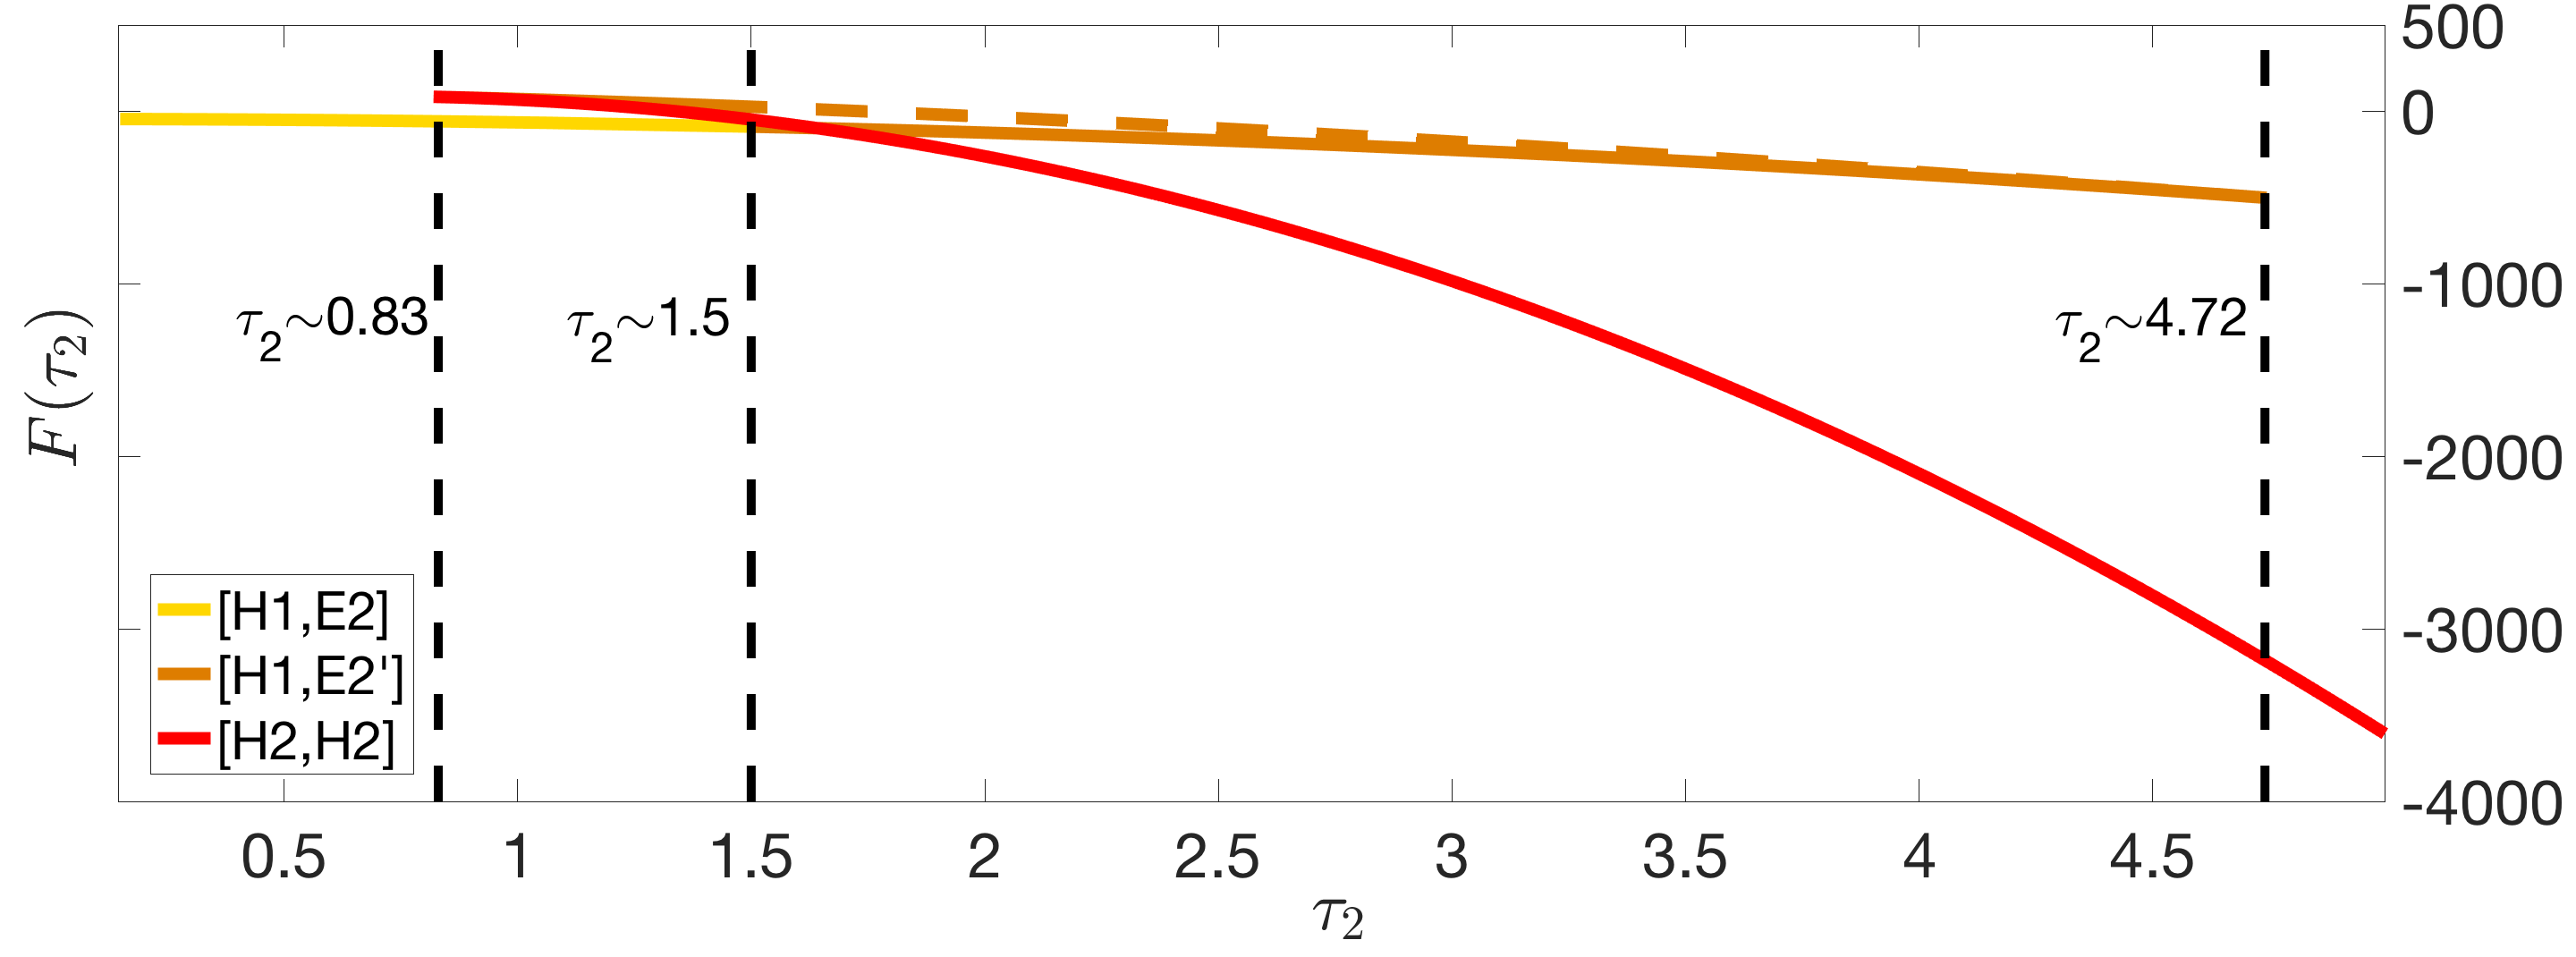
\includegraphics[width=0.9\textwidth]{figures/Free_energy_2.png}
    \caption{The free energies (\ref{free E}) of the three phases (warm and hot) as a function of $\tau_2$. The value of the free energy of $\left[\text{H}2,\text{H}2\right]$ keeps on reaching higher negative values as $\tau_2$ increases. The free energy \ref{F(E2')} takes two values for $\tau_2>1.5$ due to the shape of $f_2(\mu)$. We only consider the minimum of the two values.}
    \label{free_energie}
\end{figure}

We plotted the three free energies in figure \ref{free_energie}. We can see that as we start with low temperature, i.e lower $\tau_2$, the only phase that exist is $\left[\text{H}1,\text{E}2\right]$ while $\left[\text{H}1,\text{E}2'\right]$ and the hot phase do not appear yet. As $\tau_2$ increases, the hot phase and $\left[\text{H}1,\text{E}2'\right]$ appear, but they are dominated by $\left[\text{H}1,\text{E}2\right]$. At $2\pi\tau_2=-\Tilde{f}_2(1)$, $\left[\text{H}1,\text{E}2\right]$ ceases to exist and a continuous phase transition happens between the two warm phases. Shortly after that, the hot phase $\left[\text{H}2,\text{H}2\right]$ takes over and remains dominant for higher $\tau_2$.

\section{The Geometry of the hot phase}
The hot phase seems to dominate over the warm phases early and continues to exist for higher temperature while the warm phases cease to exist. Therefore we consider $\left[\text{H}2,\text{H}2\right]$ to be the dominant phase that we intend to study in the next chapters. We start by writing explicitly its geometry.

The geometry was already written in eq. (\ref{geometry}). In order to determine the range of the coordinates $\left(x_j,r_j\right)\in \Omega_j$, we have to solve the wall equation in section \ref{solutions}. The wall parameter $\sigma$ takes values in $(-\infty,-\sigma_+)\cup(\sigma_+, \infty)$. In the case of the hot phase $\sigma_+=0$. From eq. (\ref{solution r}), we can see that $r_j$ takes values in $(\ell_j\sqrt{M_j},\infty)$, which are exactly the values outside the horizon. Regularity of the geometry requires $M_1=M_2=(2\pi T)^2$.

\begin{figure}
    \centering
    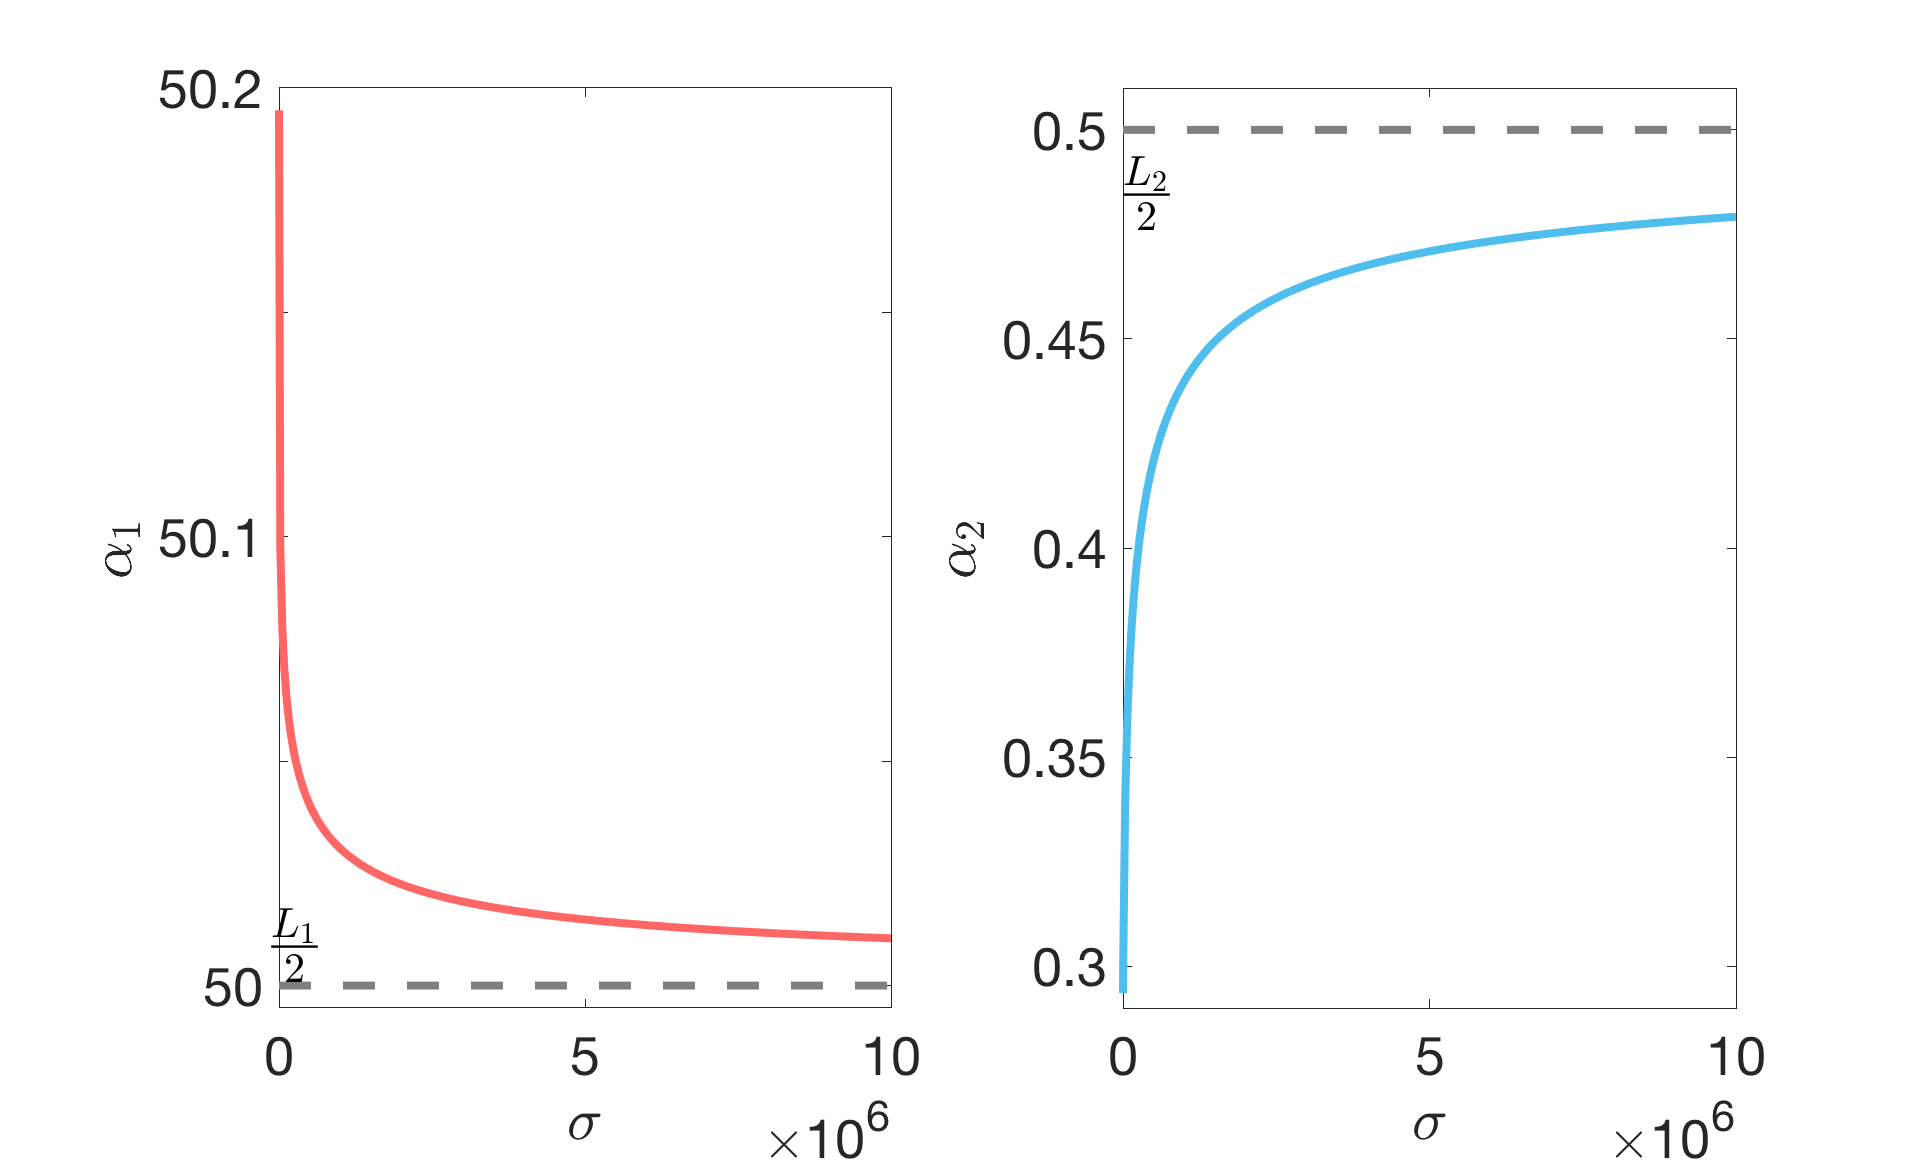
\includegraphics[width=0.9\textwidth]{figures/alpha.png}
    \caption{Plots of the function $\alpha_j(\sigma)$ for both slices in the hot phase $\left[\text{H}2,\text{H}2\right]$ solution. We chose a $\ell_2=10\ell_1$, $L_1=100\cdot L_2=100$ and a temperature where the hot phase dominates $\tau_2=2$. Both curves converge to $L_j/2$ as a result of the choice of the constant $c_j$.}
    \label{alpha_sigma}
\end{figure}

The solutions (\ref{solution x1}) and (\ref{solution x2}) give the limiting values of $x_j$. Since we are working in a symmetric geometry with respect to $\sigma = \sigma_+$, $x_j(\sigma)$ will take values in $]-\alpha_j(\sigma),\alpha_j(\sigma)[$ where $\alpha_j(\sigma)$ is given, up to a constant, by integrating eq. (\ref{solution x1}) and (\ref{solution x2}),
\begin{subequations}\label{mysolved}
\begin{align}
    \alpha_1(\sigma) = \frac{1}{2\pi T}\tanh^{-1}\left(\frac{\ell_1\left(\lambda^2+{\lambda_0}^2\right)}{2\lambda}\frac{1}{\sqrt{a_1\sigma+1}}\right) + c_1,\label{solved x1}\\
    \alpha_2(\sigma) = \frac{1}{2\pi T}\tanh^{-1}\left(\frac{\ell_2\left(\lambda^2-{\lambda_0}^2\right)}{2\lambda}\frac{1}{\sqrt{a_2\sigma+1}}\right) + c_2,\label{solved x2}
\end{align}
\end{subequations}
where $a_j=A\ell_j^2/4\lambda^2$. The constants are irrelevant in the computations. The choice $c_j=L_j/2$\footnote{not to be confused with the central charges.} fixes $x_j=0$ in the middle of the boundary interval $L_j$. The convention we are working in is that $\sigma$ increases as we circle the plane ($r_j,x_j$) clockwise.

We plotted these two function of $\sigma$ in fig. \ref{alpha_sigma}. We chose a temperature, $M_1=M_2=\left(2\pi T\right)^2$, where the hot phase already dominates over the warm phase.

\section{Conformal Compactification}

\begin{figure}
    \centering
    \begin{subfigure}[b]{0.45\textwidth}
        \centering
        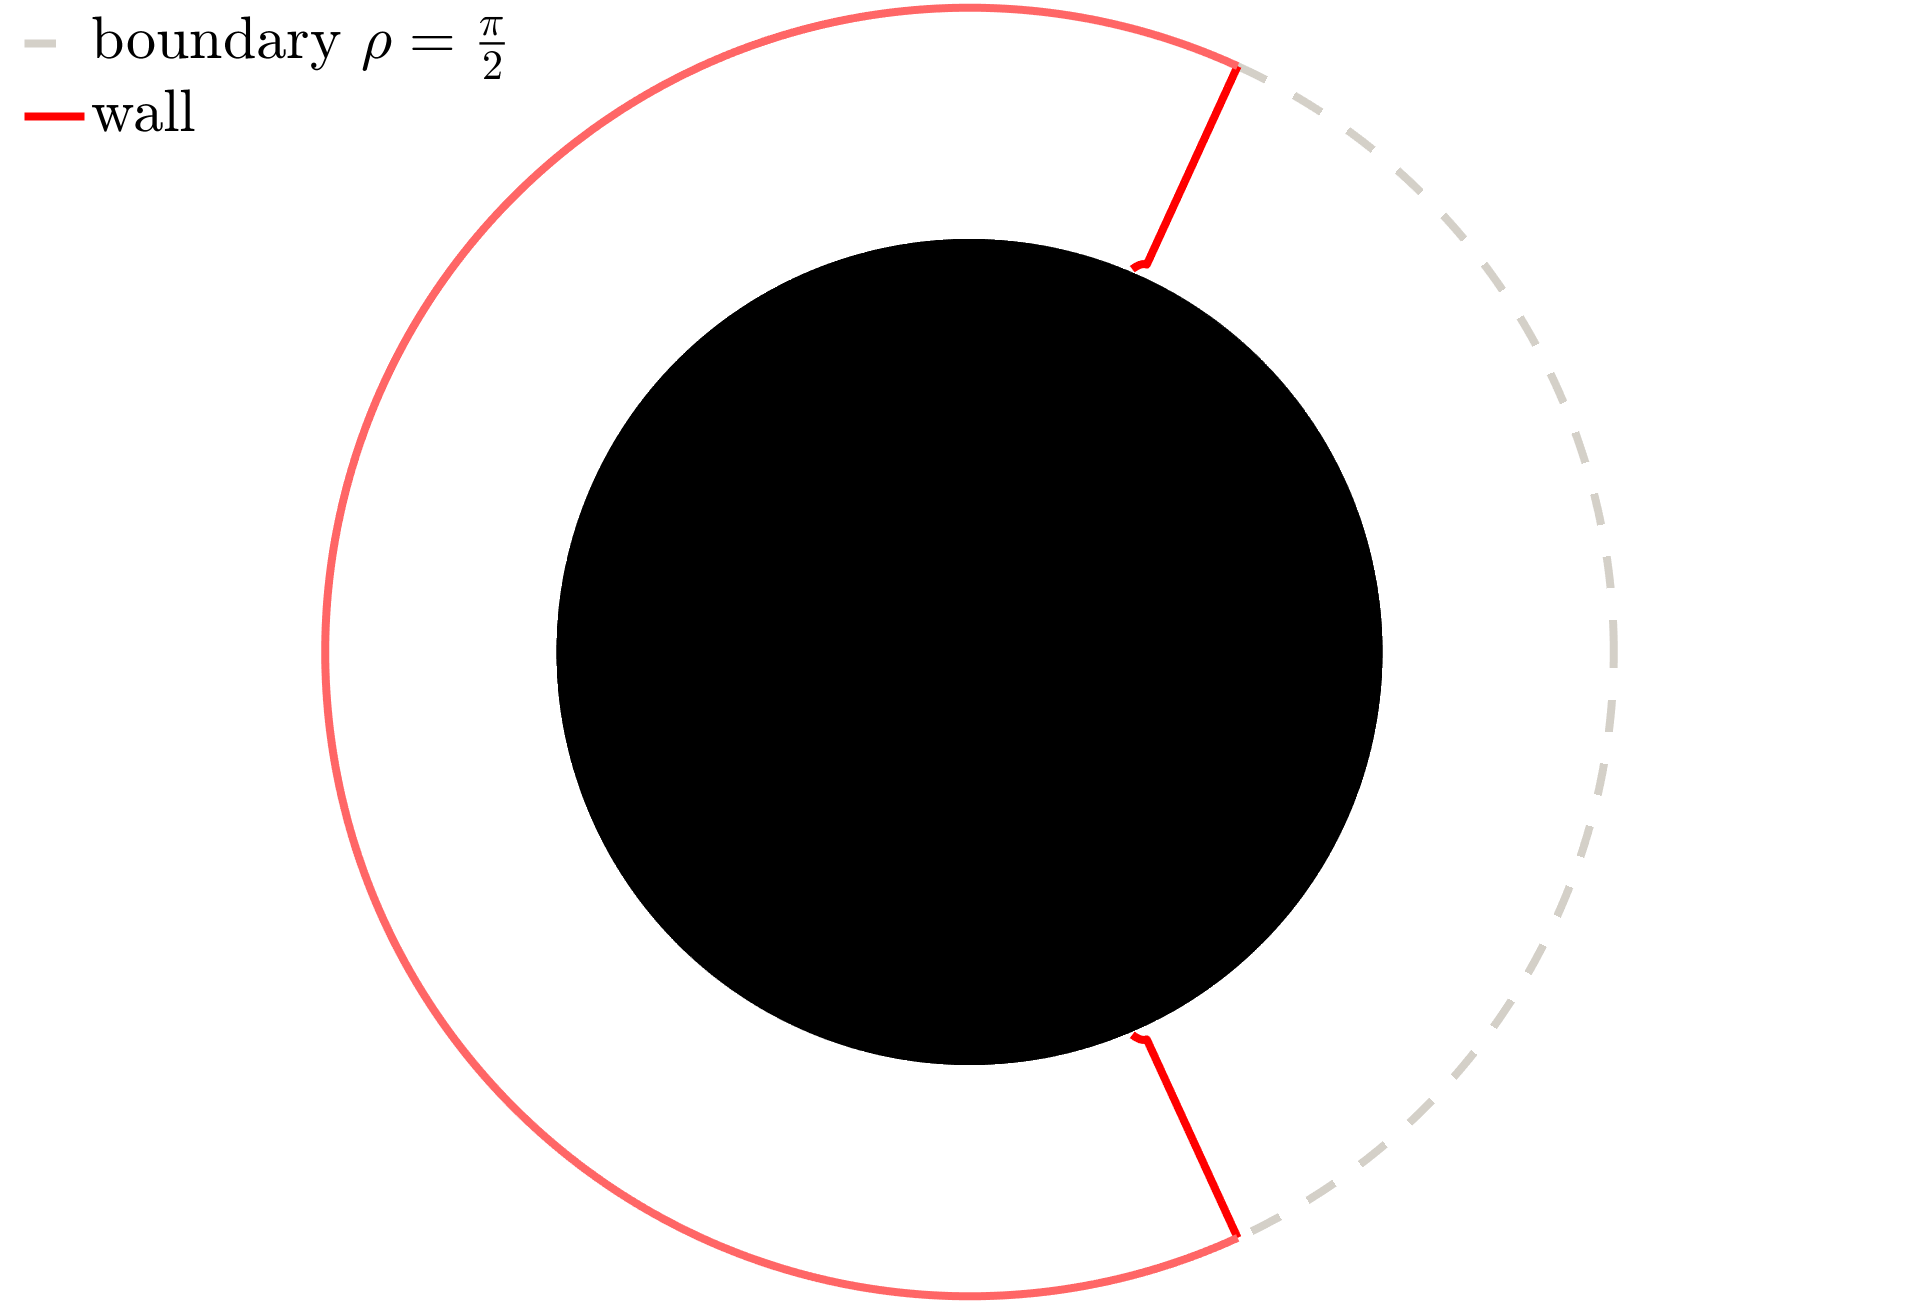
\includegraphics[width=\textwidth]{figures/wall_red.png}
        \label{wall_red}
    \end{subfigure}
    \hfill
    \begin{subfigure}[b]{0.45\textwidth}
        \centering
        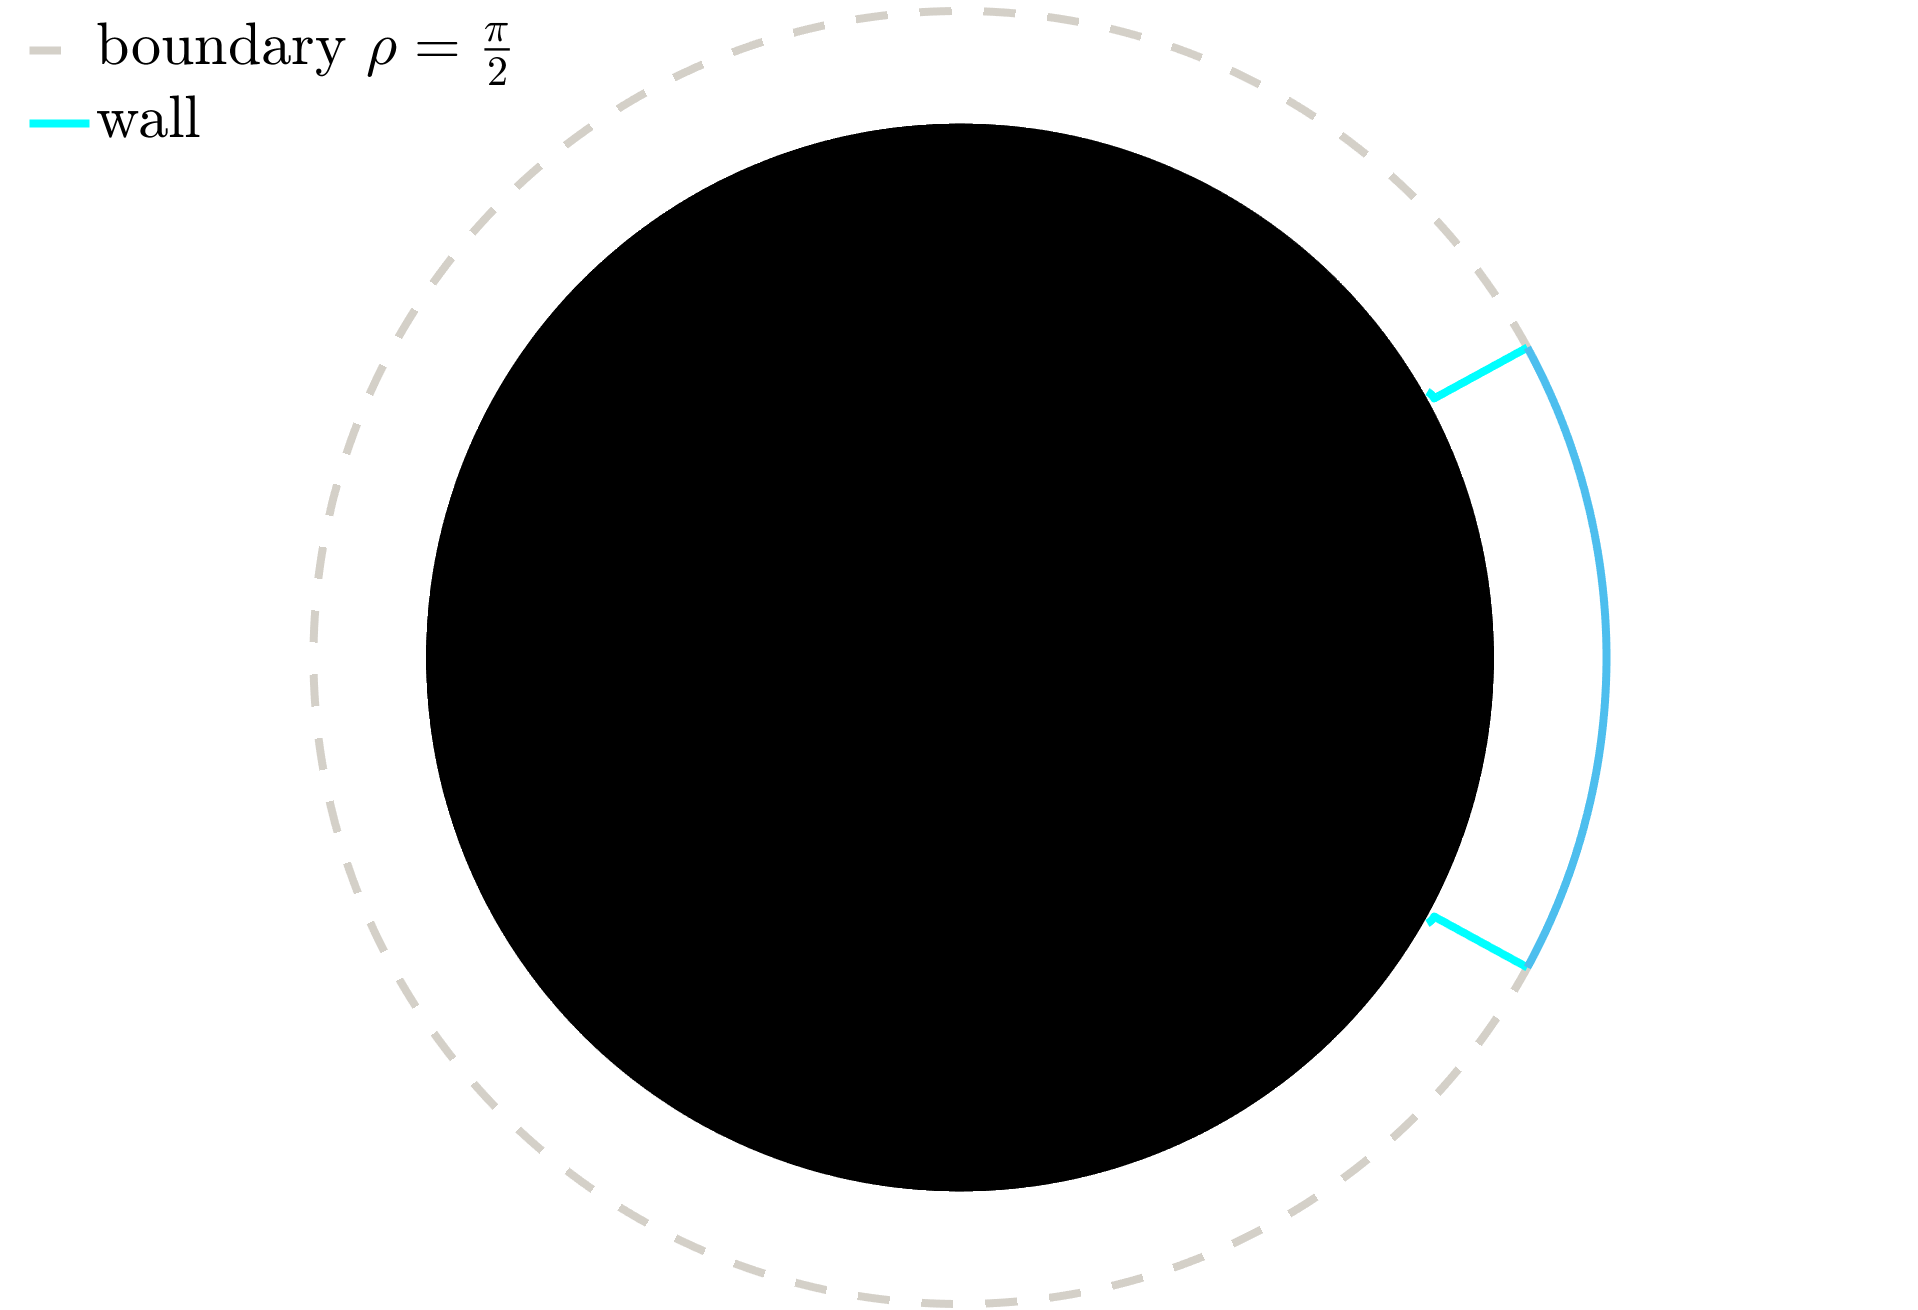
\includegraphics[width=\textwidth]{figures/wall_blue.png}
        \label{wall_blue}
    \end{subfigure}
    \caption{A plot of the wall (\ref{mysolved}) inside each slice.}
    \label{slicegeodesic}
\end{figure}


In order to get a good representation of the geometry we are working on, we make a change of variables to represent $r_j$ on a finite interval. We make the following change of coordinate,
\begin{equation}
    r=\tan{\rho}, \quad \text{where} \rho \in [0,\frac{\pi}{2}).
\end{equation}

The metric (\ref{geometry}) becomes,
\begin{equation}
    \text{d}s^2 = \frac{1}{\cos^2{\rho_j}}\left( \frac{\ell_j^2}{\sin^2{\rho_j}-M_j\ell_j^2\cos^2{\rho_j}}\text{d}\rho_j^2+\sin^2{\rho_j}\text{d}x_j^2\right)
\end{equation}
where we work at constant time, $\text{d}t=0$.

The horizon is found solving $g_{\rho\rho}^{-1}=0$, which gives $r_j = \tan\rho_j=\ell_j\sqrt{M_j}$. The conformal factor $\Omega^2(\rho_j)=\cos^{-2}(\rho_j)$ diverges at $\rho_j=\pi/2$.

The advantage of this compactification is that the representation now looks more like the spherical representations we had in previous figures. We use this change of coordinate to plot the wall solutions (\ref{mysolved}) inside the geometry. This is represented in fig. \ref{slicegeodesic}.


\addchap{Geodesics in the Single Sided Hot Phase}
\setcounter{chapter}{5}
\refstepcounter{chapter}
\label{section 6}
In this section we compute geodesics in the hot phase studied in the previous section. We apply what we learned in chapters \ref{section 2} and \ref{section 3} about RT surfaces. We split our system into two separate systems (CFT$_1$ and CFT$_2$) and compute results as if we had two boundary CFTs with an end of the world brane at the wall\cite{chu2021page}.

\section{Ryu-Takayanagi surfaces in a single slice}

We start by considering a single slice. It consists of a CFT on a an interval of length $L$ bounded by two interfaces lying on the boundary of a BTZ geometry, fig. \ref{BCFT}. Joining the two slices together is a matter of the choice of the constant $c_j$ in eq. (\ref{mysolved}). Since the geodesics lengths are independent of this choice, separating these two slices won't affect the results. This is like the situation a BCFT \cite{chu2021page} but with 2 end of the world branes instead.

\begin{figure}
    \centering
    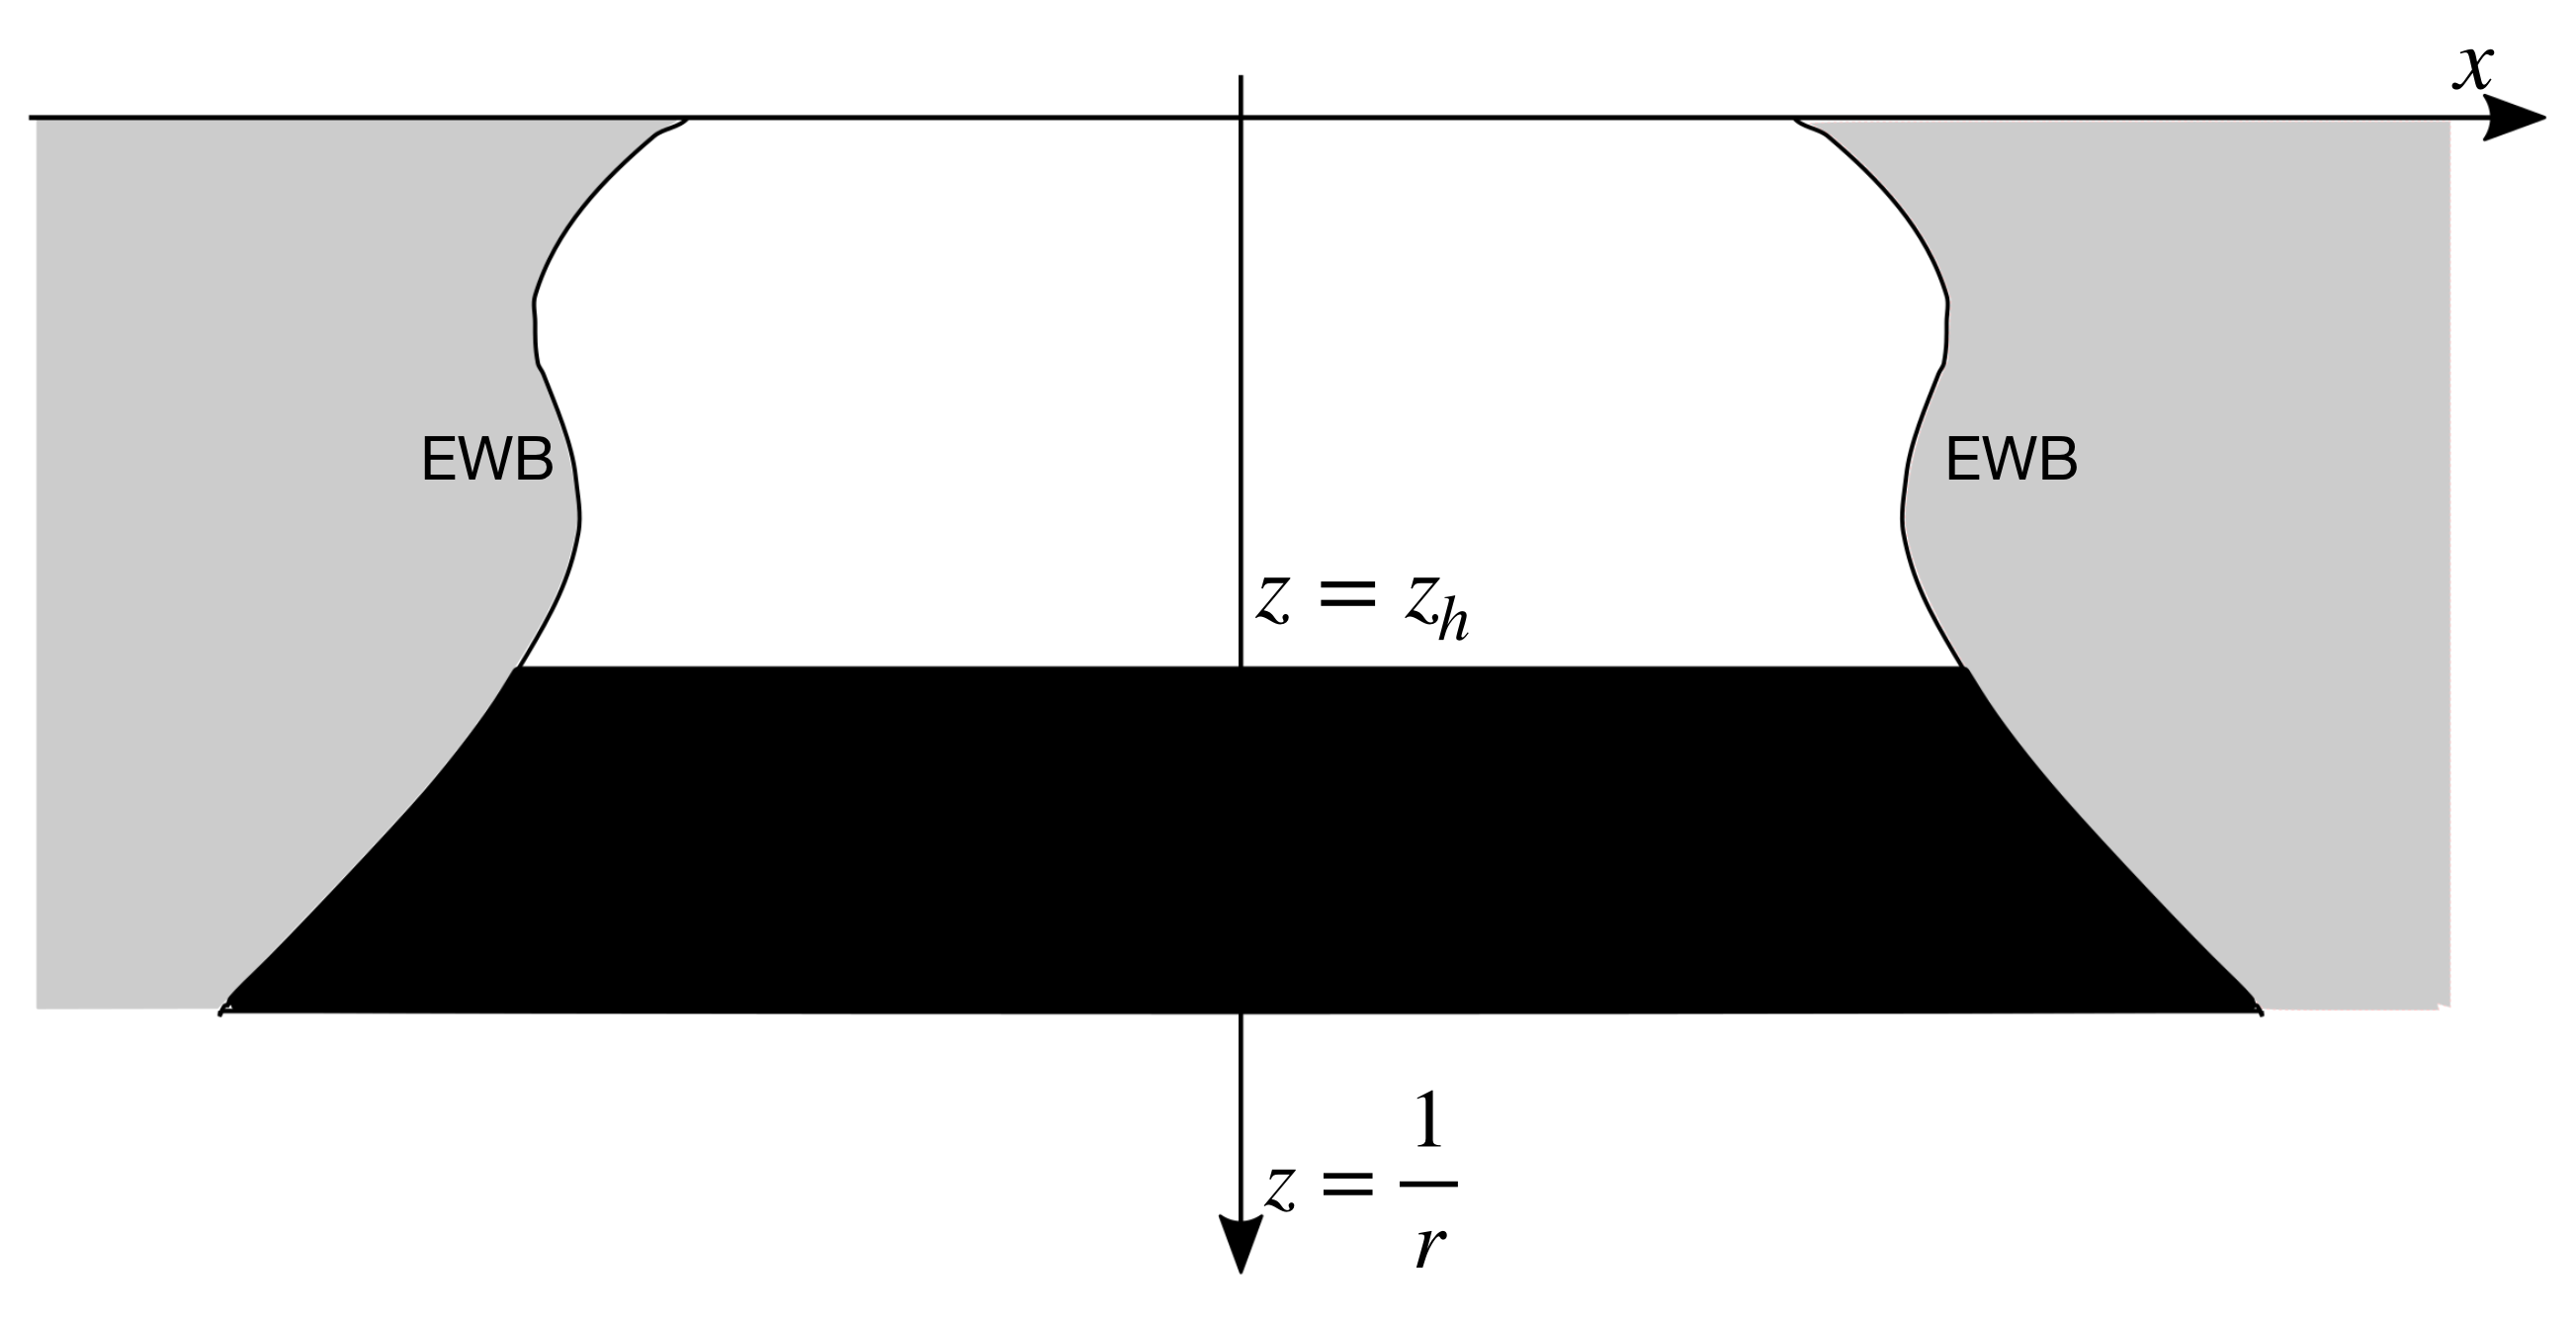
\includegraphics[width=0.9\textwidth]{figures/BCFT.png}
    \caption{BCFT with a BTZ geometry in the bulk. Since our original system features two walls, we represent here a BCFT with two end of the world branes. Here we used the (\ref{change of coord rz}) coordinates.}
    \label{BCFT}
\end{figure}

Computing RT surfaces goes back to computing space like geodesics. The geodesic equations in $(r,x)$\footnote{We don't write the slice index $j$ for clarity.} coordinates are
\begin{subequations}
    \label{geodesic equations}
    \begin{align}
        \ddot x &= -\frac{2\dot r\dot x}{r}\label{geodesic 1}\\
        \ddot r &= \frac{r\dot r}{r^2-M\ell^2} + \frac{r(r^2-M\ell^2)\dot x}{\ell^2},\label{geodesic 2}
    \end{align}
\end{subequations}
where the dot denotes a derivative with respect to the affine parameter $\lambda$.

The first equation (\ref{geodesic 1}) is just telling us that the tangential acceleration is vanishing and therefore the angular momentum is conserved,
\begin{equation}
    r^2\dot x=J.
\end{equation}

The second equation is more difficult to solve. We can treat this problem by considering the length of the geodesic between two endpoints $P_1$ and $P_2$,
\begin{equation}\label{Action}
    L = \ell\int d \phi\sqrt{\frac{r'^2}{r^2-M\ell^2}+r^2},
\end{equation}
where we made the following substitution $\phi=x/\ell$. The prime denotes a derivative with respect to $\phi$.

Treating $L$ as a one dimensional action, the energy conservation reads,
\begin{equation}
    \frac{r^2}{\sqrt{\frac{r'^2}{r^2-M\ell^2}+r^2}}= \frac{E}{\ell},
\end{equation}
where $E$ is a constant of integration. Rearranging this equation, we get,
\begin{equation}
    E^2r'^2 = \ell^2r^2(r^2-E^2)(r^2-r_h^2),
\end{equation}
where $r_h=\ell\sqrt{M}$. Integrating this equation a second time gives
\begin{equation}\label{solution phi}
    r(x) = \frac{E}{r_h\ell}\frac{1}{\sqrt{\frac{E^2}{r_h^2\ell^2}\cosh^2\left(r_h\frac{x}{\ell}+c\right)-\sinh^2\left(r_h\frac{x}{\ell}+c\right)}}
\end{equation}
where $c$ is a constant of integration and can be set to 0 if we consider symmetric geodesics with respect to $x = 0$. Two geodesics are drawn in  fig. \ref{geodesic pic} between two infinite points separated by an arc of length $2x_0$ as well as two points on the wall. We impose different boundary conditions for each geodesic to find $E$.

Integrating (\ref{Action}) using (\ref{solution phi}), we find the length of the geodesic homologous to an interval of length $2x_0\ll L$ on the boundary,
\begin{equation}\label{S1}
    2\ell\log\left(\frac{\beta}{\pi\ell\epsilon}\cosh\left(\frac{\pi 2x_0 }{\beta}\right)\right),
\end{equation}
where we used $r_h=\frac{2\pi\ell}{\beta}$.

This is similar to what we find in eq. (\ref{length BTZ red}). The corresponding entanglement entropy is given by the RT formula,
\begin{equation}
    S = \frac{c}{3}\log\left(\frac{\beta}{\pi\ell\epsilon}\cosh\left(\frac{\pi 2x_0 }{\beta}\right)\right).
\end{equation}

\begin{figure}
    \centering
    \begin{subfigure}[b]{0.45\textwidth}
        \centering
        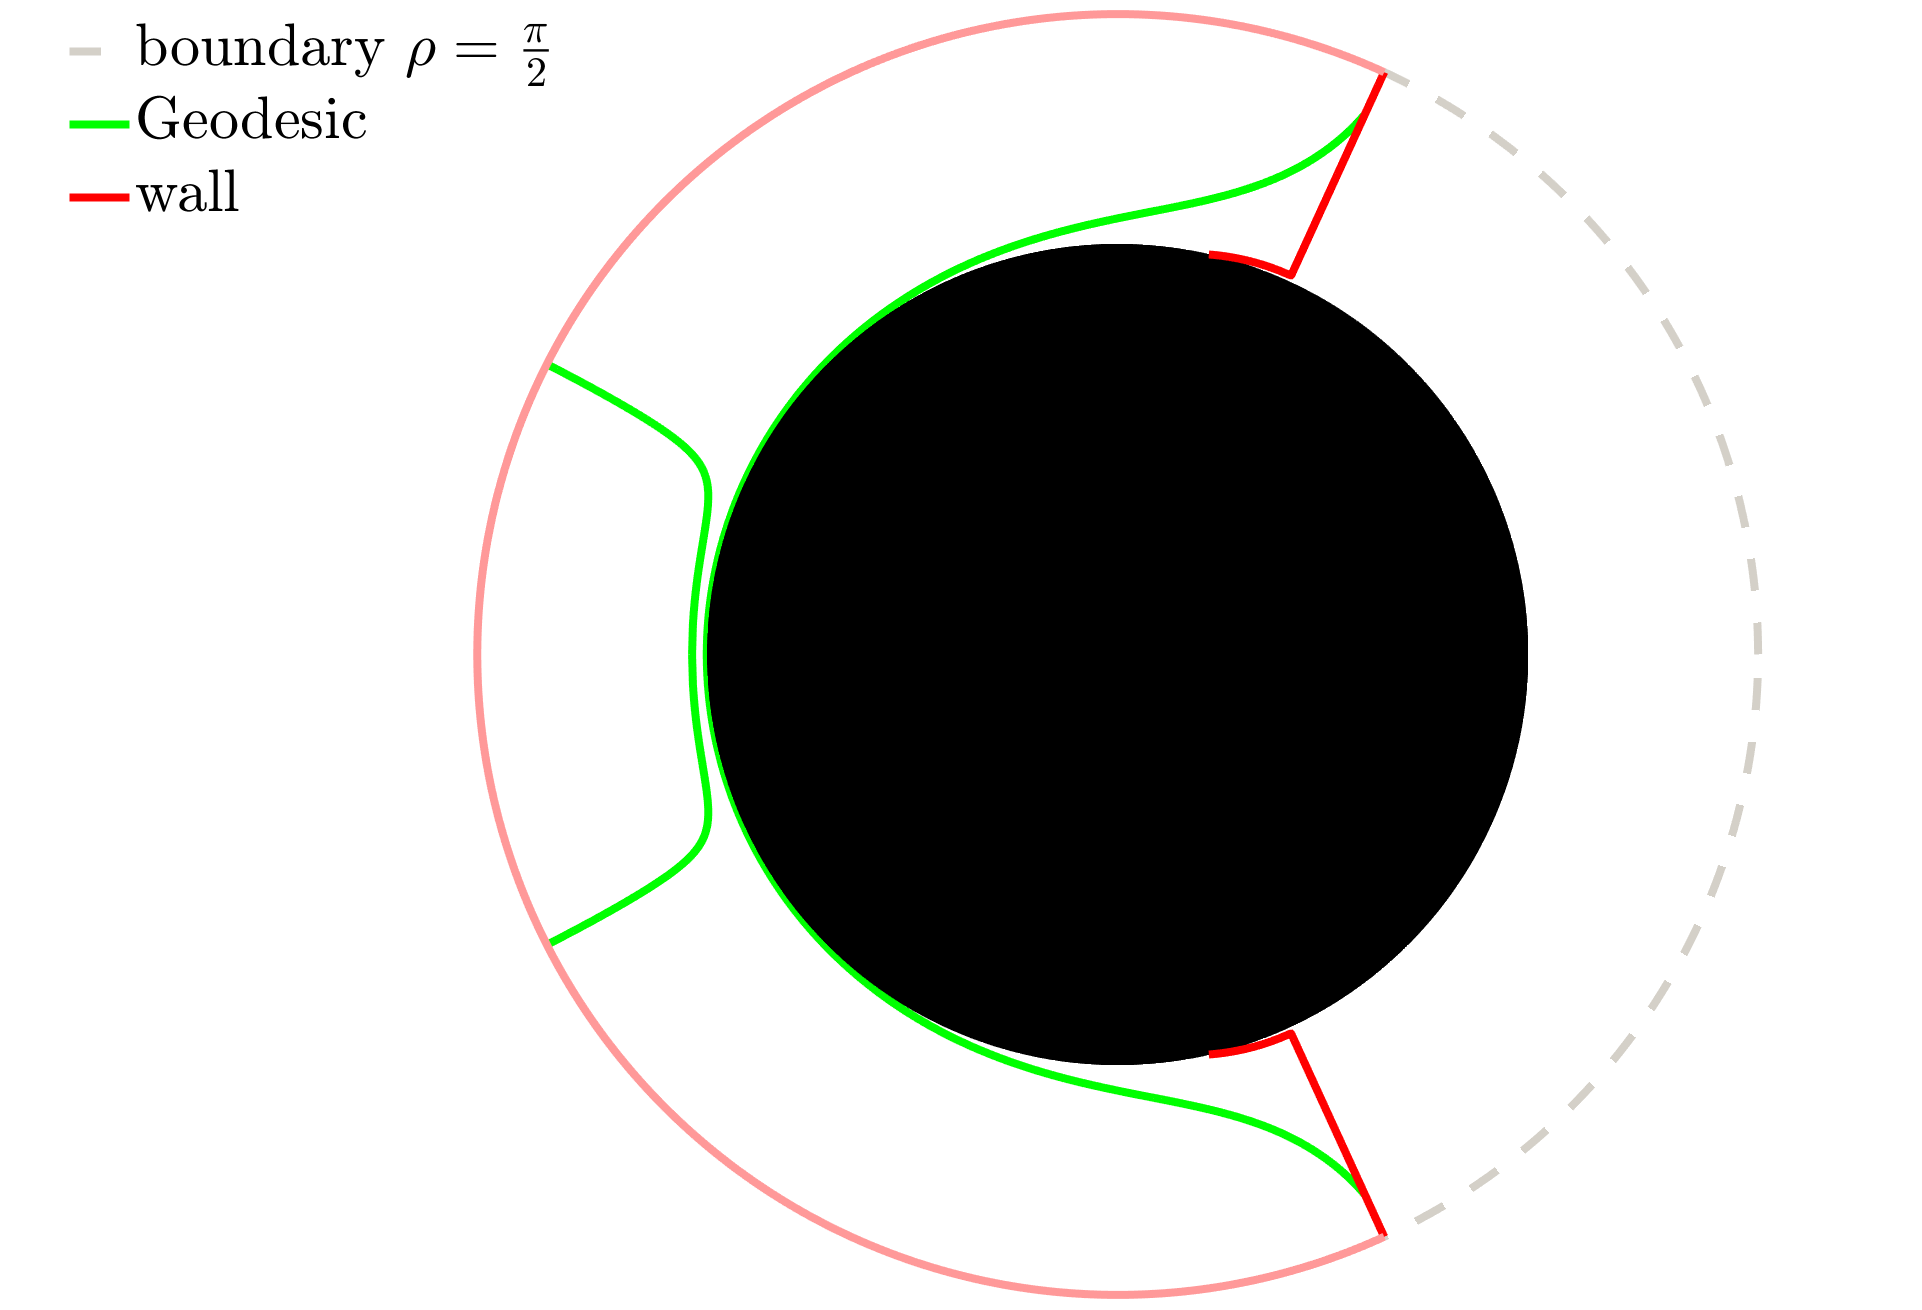
\includegraphics[width=\textwidth]{figures/geodesic_red.png}
        \label{greengeodesic}
    \end{subfigure}
    \hfill
    \begin{subfigure}[b]{0.45\textwidth}
        \centering
        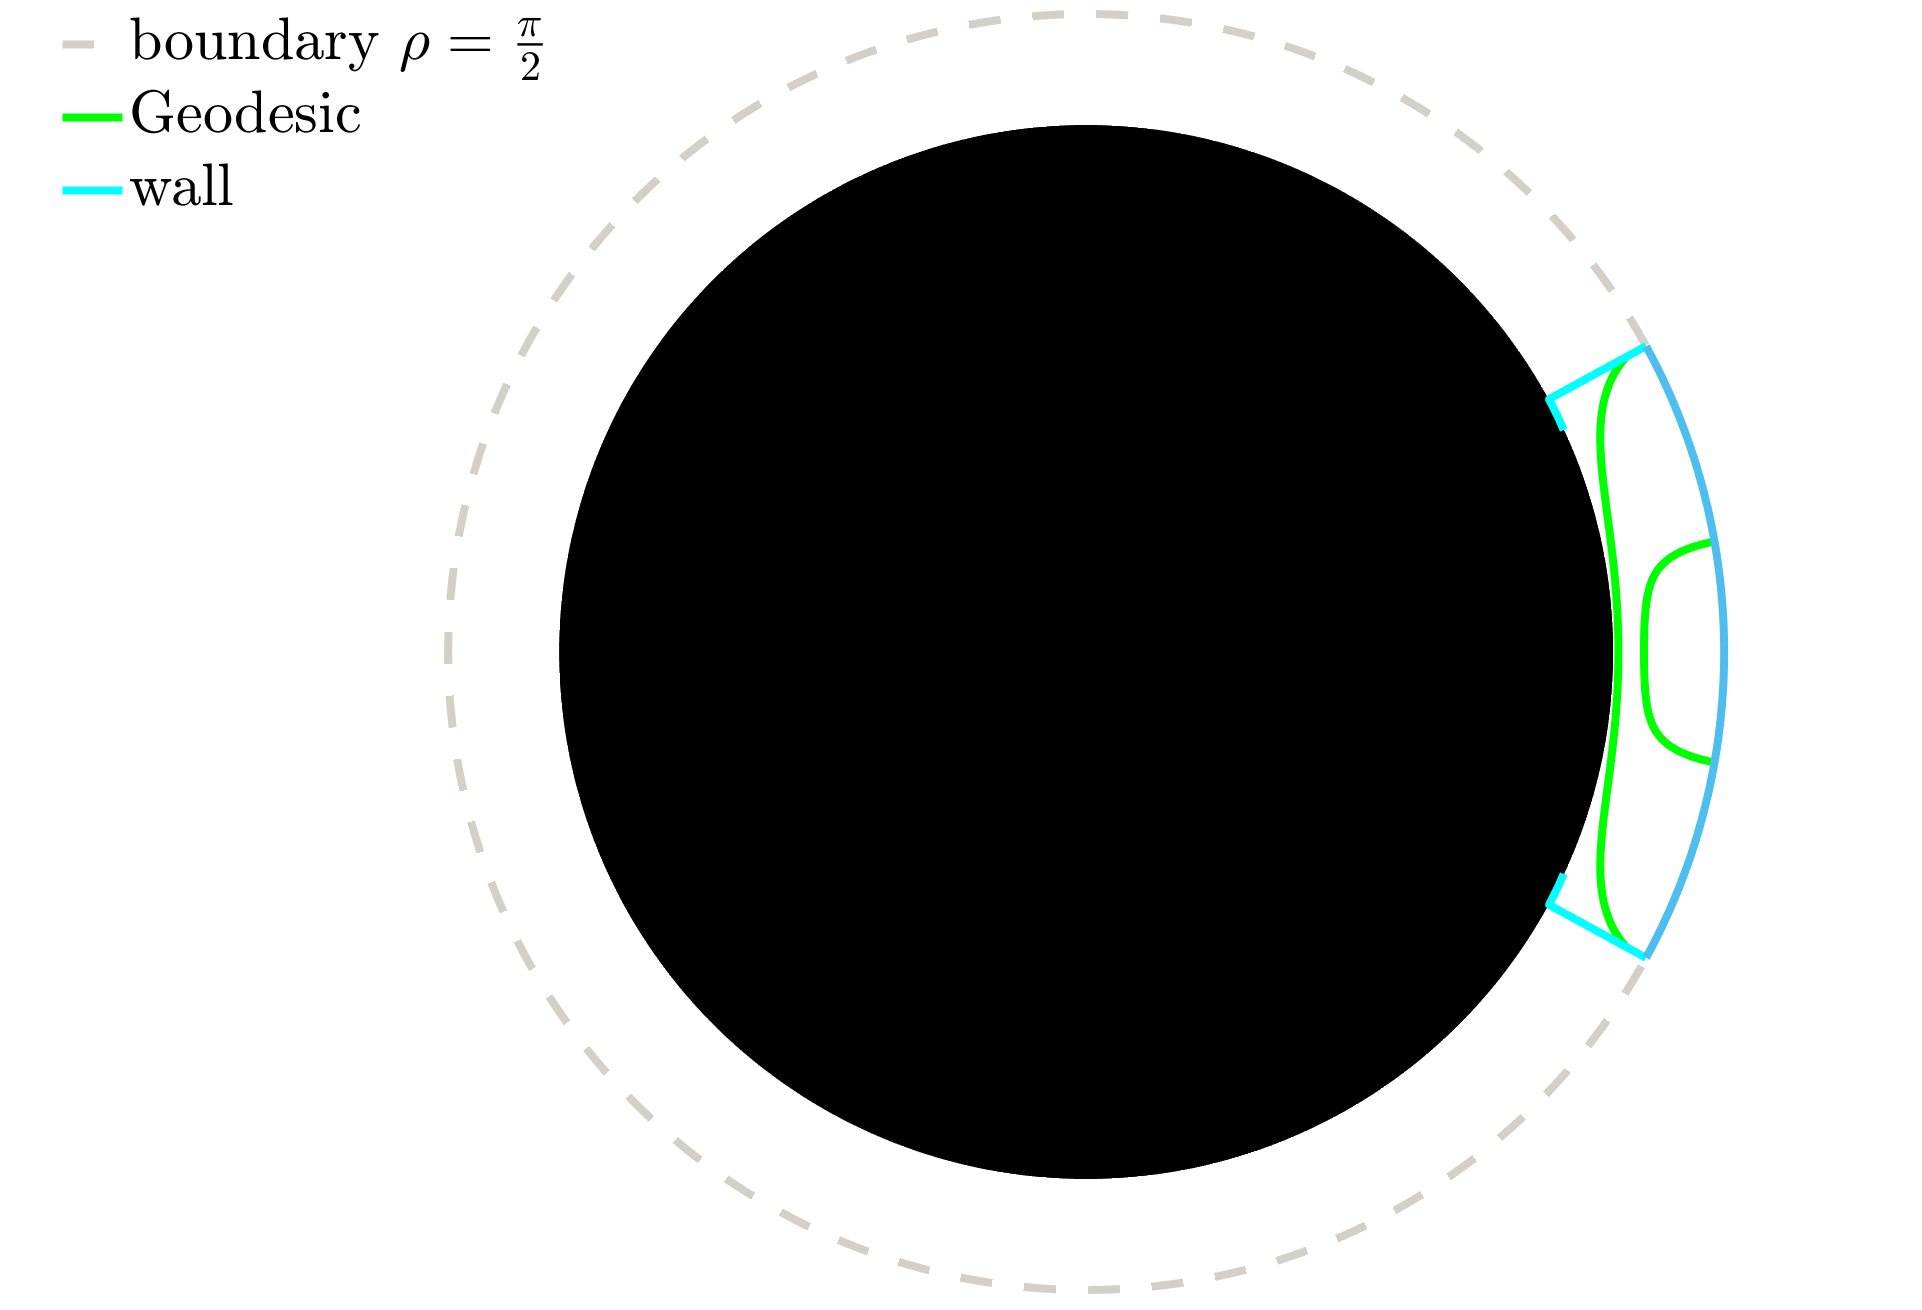
\includegraphics[width=\textwidth]{figures/geodesic_blue.png}
        \label{pinkgeodesic}
    \end{subfigure}
        \caption{Geodesics inside each slice between two symmetric points. One geodesic has its endpoints on the boundary, the other on the wall. For the red slice the geodesic with the the endpoints on the wall asymptotes the Horizon. We chose $\ell_2/\ell_1=1.5$.}
        \label{geodesic pic}
\end{figure}

\section{Ryu-Takayanagi surfaces in the hot phase}

The system we are working on $[\text{H}2,\text{H}2]$ resembles a lot that of fig. \ref{fig_BTZ minimal surface}. In fact it is the same with the addition of a wall with different central charges on each side. Therefore, the computation of RT surfaces is somewhat similar to those in chapter \ref{section 3}, with the first possibility already computed in the previous section and the second one slightly different than eq. (\ref{second entropy}). 

More precisely, we compute the EE of the blue slice with a large number of degrees of freedom $c_2$ as was depicted in fig. \ref{QM 2}. The EE is that of an interval $A$ which includes all of $L_2$ and an finite part of $L_1$ of size $h$ of the same order as $L_2$. The RT surfaces correspond to geodesics linking two symmetric points on the red slice boundary. They can be of two kinds: either they stay in the same slice (the red one) or they cross the wall. The two possible situations that we have are represented in fig. \ref{2 situations}. The first case fig. \ref{case1} is the one computed in the previous section. For the RT surface to be homologous to the boundary region $A$, we add the horizon surface as was discussed in chapter \ref{section 3}. The EE is,
\begin{equation}
    S = \frac{c}{3}\log\left(\frac{\beta}{\pi\ell\epsilon}\cosh\left(\frac{\pi h }{\beta}\right)\right) + S\left(\mathcal{H}\right),
\end{equation}
where $S\left(\mathcal{H}\right) = 2\pi \left({r_h}_1\Delta x_1\big|_\text{hor}+{r_h}_2\Delta x_2\big|_\text{hor}\right)$. The $\Delta x_j\big|_\text{hor}$ are computed through eq (\ref{mysolved}).

\begin{figure}
     \centering
     \begin{subfigure}[b]{0.4\textwidth}
         \centering
         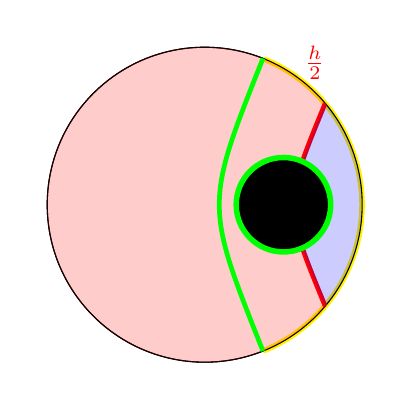
\begin{tikzpicture}
    \draw[name path = A] (1.53,-1.288) arc (319.9:400.09:2);
    \draw[name path = AA] (1.53,1.288) arc (40.09:319.9:2);
    \draw[yellow, line width=2, opacity=1] (0.74,-1.858) arc (291.79:427.9:2);    
            \begin{scope}
                \draw  [clip] (0,0) circle (2cm);
                \draw[color=red,line width=.6mm, name path = B] (1.53,-1.288) .. controls (1,0) .. (1.53,1.288);
                
                %\draw[color=blue,line width=.6mm, name path = R] (1.53,-1.288) .. controls (0,0) .. (1.53,1.288);
                \tikzfillbetween[of=A and B]{blue, opacity=0.2};
                \tikzfillbetween[of=AA and B]{red, opacity=0.2};
                \draw[color=green,line width=.6mm] (0.74,1.858) .. controls (0,0) .. (0.74,-1.858);
            \end{scope}
            \draw[red] node at (1.4,1.8){$\frac{h}{2}$};
            \draw[blue] node at (-2,-1){};
            \draw[green,fill=black, line width =2] (1,0) circle (.6cm);
            
         \end{tikzpicture}
         \caption{Geodesic outside the wall}
         \label{case1}
     \end{subfigure}
     \hfill
     \begin{subfigure}[b]{0.4\textwidth}
         \centering
         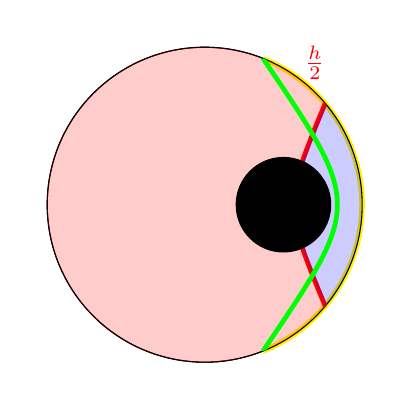
\begin{tikzpicture}
    \draw[name path = A] (1.53,-1.288) arc (319.9:400.09:2);
    \draw[name path = AA] (1.53,1.288) arc (40.09:319.9:2);
    \draw[yellow, line width=2] (0.74,-1.858) arc (291.79:427.9:2);    
            \begin{scope}
                \draw  [clip] (0,0) circle (2cm);
                \draw[color=red,line width=.6mm, name path = B] (1.53,-1.288) .. controls (1,0) .. (1.53,1.288);
                
                %\draw[color=blue,line width=.6mm, name path = R] (1.53,-1.288) .. controls (0,0) .. (1.53,1.288);
                \tikzfillbetween[of=A and B]{blue, opacity=0.2};
                \tikzfillbetween[of=AA and B]{red, opacity=0.2};
                \draw[color=green,line width=.6mm] (0.74,1.858) .. controls (2,0) .. (0.74,-1.858);
            \end{scope}
            \draw[red] node at (1.4,1.8){$\frac{h}{2}$};
            \draw[blue] node at (-2,-1){};
            \draw[black,fill=black] (1,0) circle (.6cm);
            
         \end{tikzpicture}
         \caption{Geodesic traversing the wall}
         \label{case2}
     \end{subfigure}
        \caption{The interval of the system with large central charge $A=L_2+h$ is highlighted in yellow. The green line is its corresponding RT surface. The RT surfaces are symmetric with respect to $\sigma=0$.}
        \label{2 situations}
\end{figure}

For the case \ref{case2}, we have to break down the geodesic into three subgeodesics as depicted in fig. \ref{case2separated}. The sum of the three subgeodesics is a function of the wall parameter $\sigma$. The final EE is found by minimizing over $\sigma$,
\begin{equation}\label{second entropy}
    S'\left(A\right) = \min_\sigma\left\{2S\left(\gamma_1(\sigma)\right)+S\left(\gamma_2(\sigma)\right)\right\}.
\end{equation}

The geodesic $\gamma_1(\sigma)$ is a geodesic linking a fixed point in $\partial A$ and a moving point on the wall ($r_1(\sigma),x_1(\sigma)$). The geodesic $\gamma_2(\sigma)$ is a geodesic linking two moving points on the wall, ($r_2(\sigma),x_2(\sigma)$) and ($r_2(\sigma),-x_2(\sigma)$).

Using eq.(\ref{solution phi}), we compute the length of the two geodesics. On the red slice\footnote{On the red slice, we prefer to integrate over $r_1$ rather than $x_1$. Constants of integration are easier to compute this way.} we get,
\begin{equation}
    \gamma_1(\sigma)=\ell_1\left(\ln\left(\frac{2}{\epsilon}\right)-\ln\left(\sqrt{\sigma}+\sqrt{\sigma+{r_h}_1^2-\frac{J_1(\sigma)^2}{\ell_1^2}}\right)\right),
\end{equation}
where $J_1(\sigma)$ is a $\sigma$ dependent constant of integration which solves,
\begin{equation}\label{maconstante}
    \tanh \left( {r_h}_1 \frac{2x_1(\sigma) - A}{2\ell_1}\right) = \frac{C(\sigma)-D(\sigma)}{1-C(\sigma)D(\sigma)},
\end{equation}
with $C(\sigma)$ and $D(\sigma)$ two functions,
\begin{align}\label{CD}
    C(\sigma) &= \frac{J_1(\sigma)}{r_{h_1}\ell_1}, \\
    D(\sigma) &= \frac{J_1(\sigma)}{r_{h_1}\ell_1}\sqrt{\frac{\sigma}{\sigma+r_h_1^2-J_1(\sigma)/\ell_1}}.
\end{align}
%2\ell_2\left(\ln\left(\sqrt{\sigma}+\sqrt{\sigma+{r_h}_2^2-E_2(\sigma)^2}\right)-\frac{1}{2}\ln\left(E_2(\sigma)^2-{r_h}_2^2\right)\right),%

On the blue slice we get,
\begin{equation}
    \gamma_2(\sigma)=\frac{2\ell_2}{r_h_2^2}\tanh^{-1}\left(\frac{r_h_2\ell_2}{E_2(\sigma)}\tanh\left(\frac{r_h_2x_2(\sigma)}{\ell_2}\right)\right)
\end{equation}
where $E_2(\sigma)$ is the blue slice's constant of integration computed in appendix \ref{appendix D}.

There is however one problem we might run into. In the process of computing the geodesics above, we don't take into account that the wall is restricting our space. Therefore, some geodesics of $\gamma_i$ may traverse the wall before reaching the final endpoint $P(\sigma)$ and therefore have a part in the other slice. These geodesics should not be considered as solutions. We should restrict our solutions to $(x_i,r_i)\in D_i$ where $D_i=[0,\alpha_i(r)]\times[{r_h}_i,\infty]$. Here we have considered the symmetry of our geodesics and work with the upper part of the slice $x_i\geq0$. In such situations the real space-like geodesic is
\begin{equation}
    \Tilde{\gamma}_i(\sigma) = \min\{\gamma_i(\sigma)\subset D_i\} \geq \gamma_i(\sigma).
\end{equation}

In order to force our Lagrangian (\ref{Action}) to give geodesics inside the desired slice we can add a constant infinite term on the other side of the wall,
\begin{equation}
    \mathcal{L}\left({x'}_i(r_i),x_i(r_i),r_i\right) \to \mathcal{L}\left({x'}_i(r_i),x_i(r_i),r_i\right) + \beta\,\Theta\left( x_i(r_i) - \alpha_i(r_i)\right),
\end{equation}
Here we switched to $r$ as the Lagrangian time,
\begin{equation}
    \mathcal{L}\left({x'}_i(r_i),x_i(r_i),r_i\right) = \sqrt{\frac{1}{r_i^2-r_h_i^2}+r_i^2\frac{{x'}_i}{\ell_i}}.
\end{equation}

This excludes the region outside the desired slice if we formally let $\beta \to \infty$. The differential equation to solve stays pretty much the same in the bulk but has an additional delta function in the wall region. Physically, you can think of it as a particle travelling in a space like region, when it reaches the wall, the particle finds an impenetrable barrier and bounces back. The particle then keeps on bouncing back and forth until it reaches the final destination. This is pretty much like a particle trapped in an infinite potential well.

\begin{figure}
    \centering
    \begin{subfigure}[b]{0.3\textwidth}
        \centering
        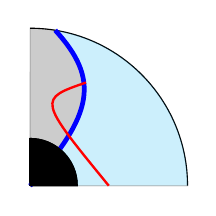
\begin{tikzpicture}
        \draw[name path = AA] (2,0) arc (0:90:2);
        \draw[fill=black,opacity=0.2,name path = Ax] (0,0) .. controls (.81,.91) and (0.89,1.35) .. (0.32,1.974) arc (80.8:90:2) -- (0,0);
        \draw[name path = z] (0.6,0) arc (0:90:0.6);
        \draw[name path = x] (0,0) -- (.6,0);
        \draw[name path = y] (0,0) -- (0,.6);
        \draw[fill=cyan,opacity=0.2,name path = Ay] (0,0) .. controls (.81,.91) and (0.89,1.35) .. (0.32,1.974) arc (80.8:0:2) -- (0,0);
            \begin{scope}
                \draw[color=blue,line width=.6mm, name path = B] (0,0) .. controls (.81,.91) and (0.89,1.35) .. (0.32,1.974);
                \draw[color=red,line width=.3mm, name path = C] (1,0) .. controls (.1,1.1) .. (0.71,1.31);
                \tikzfillbetween[of= y and z]{gray, opacity=0.2};
            \end{scope}
            \draw[fill=black] (0,0) -- (0.6,0) arc (0:90:0.6) -- (0,0);
    \end{tikzpicture}
    \caption{}
    \label{line 1}
    \end{subfigure}
    \hfill
    \begin{subfigure}[b]{0.3\textwidth}
        \centering
        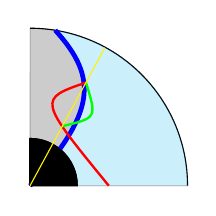
\begin{tikzpicture}
        \draw[name path = AA] (2,0) arc (0:90:2);
        \draw[fill=black,opacity=0.2,name path = Ax] (0,0) .. controls (.81,.91) and (0.89,1.35) .. (0.32,1.974) arc (80.8:90:2) -- (0,0);
        \draw[fill=cyan,opacity=0.2,name path = Ay] (0,0) .. controls (.81,.91) and (0.89,1.35) .. (0.32,1.974) arc (80.8:0:2) -- (0,0);
        \draw[name path = z] (0.6,0) arc (0:90:0.6);
        \draw[name path = x] (0,0) -- (.6,0);
        \draw[name path = y] (0,0) -- (0,.6);
            \begin{scope}
                \draw[color=blue,line width=.6mm, name path = B] (0,0) .. controls (.81,.91) and (0.89,1.35) .. (0.32,1.974);
                \draw[color=red,line width=.3mm, name path = C] (1,0) .. controls (.1,1.1) .. (0.71,1.31);
                \draw[color=green,line width=.3mm, name path = C] (0.41,0.75645) .. controls (.85,.86) .. (0.71,1.31);
                \tikzfillbetween[of= y and z]{gray, opacity=0.2};
            \end{scope}
            \draw[fill=black] (0,0) -- (0.6,0) arc (0:90:0.6) -- (0,0);
            \draw[yellow] (0,0) -- (.95,1.75275);
    \end{tikzpicture}
    \caption{}    
    \label{line 2}
    \end{subfigure}
    \hfill
    \begin{subfigure}[b]{0.3\textwidth}
        \centering
        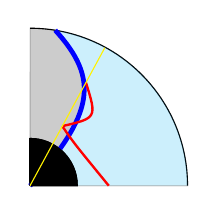
\begin{tikzpicture}
        \draw[name path = AA] (2,0) arc (0:90:2);
        \draw[fill=black,opacity=0.2,name path = Ax] (0,0) .. controls (.81,.91) and (0.89,1.35) .. (0.32,1.974) arc (80.8:90:2) -- (0,0);
        \draw[fill=cyan,opacity=0.2,name path = Ay] (0,0) .. controls (.81,.91) and (0.89,1.35) .. (0.32,1.974) arc (80.8:0:2) -- (0,0);
        \draw[name path = z] (0.6,0) arc (0:90:0.6);
        \draw[name path = x] (0,0) -- (.6,0);
        \draw[name path = y] (0,0) -- (0,.6);
            \begin{scope}
                \draw[color=blue,line width=.6mm, name path = B] (0,0) .. controls (.81,.91) and (0.89,1.35) .. (0.32,1.974);
                \draw[color=red,line width=.3mm, name path = C] (1,0) .. controls (.55,.55) .. (0.41,0.75645);
                \draw[color=red,line width=.3mm, name path = C] (0.41,0.75645) .. controls (.85,.86) .. (0.71,1.31);
                \tikzfillbetween[of= y and z]{gray, opacity=0.2};
            \end{scope}
            \draw[fill=black] (0,0) -- (0.6,0) arc (0:90:0.6) -- (0,0);
            \draw[yellow] (0,0) -- (.95,1.75275);
    \end{tikzpicture}
    \caption{}
    \label{line 3}
    \end{subfigure}
    \caption{(a) Geodesic in red in the blue slice traversing the wall. (b) a radius(yellow) passing through the endpoint of the geodesic. The red part of the geodesic on the left side of the radius is reflected and represented in green. (c) The new geodesic after the first reflection. This new geodesic has the same length as the original one. We continue on reflecting the part of the geodesic that is still outside the blue slice in the same way until nothing is left outside.}
    \label{reflection}
\end{figure}

Putting all of this together we get,
\begin{equation}\label{S2}
    S'\left(A\right) = 2\pi\left[\min_\sigma\left\{2\gamma_1(\sigma)+\gamma_2(\sigma)\right\}\right].
\end{equation}

In fact, this trajectory can be explained using the circular symmetry of our geometry. Thanks to the circular symmetry, the geometry looks the same on both sides of any drawn radius. Using this trick, we can show that there exist a path that is completely inside the desired slice that has the same length as the original geodesic.

We start by drawing a radius that goes through $P(\sigma)$ and draw the mirror image of the geodesic part that lies behind the radius as shown in figure (\ref{reflection}). We then do the same thing for the rest of the curve that still lies behind the wall until every small part is reflected inside the pink slice. The final trajectory looks like that of a particle bouncing back and forth on the wall. Since the reflected trajectories are symmetric to the original one, they have the same length. Therefore for every geodesic, there exist one that is inside the desired region which has the same length as a normal geodesic,
\begin{equation}
    \Tilde{\gamma}_i(\sigma) = \gamma_i(\sigma).
\end{equation}

The EE of Radiation will be the minimum of the two forms (\ref{S1}) and (\ref{S2}). In the limit of large $L_1$, (\ref{S1}) will be larger than (\ref{S2}). The latter has its minimal value at the horizon ($\sigma=0$) when taking the limit  $\ell_1\ll\ell_2$.

\begin{figure}
    \centering
    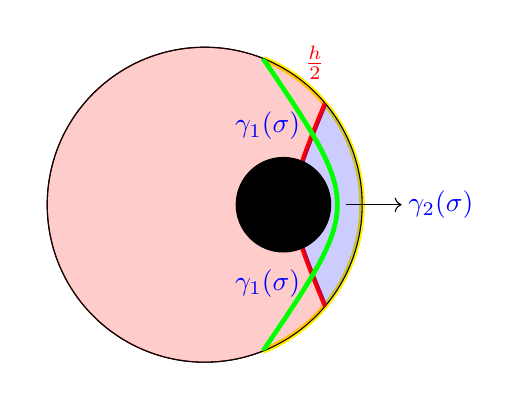
\begin{tikzpicture}
    \draw[name path = A] (1.53,-1.288) arc (319.9:400.09:2);
    \draw[name path = AA] (1.53,1.288) arc (40.09:319.9:2);
    \draw[yellow, line width=2] (0.74,-1.858) arc (291.79:427.9:2);    
            \begin{scope}
                \draw  [clip] (0,0) circle (2cm);
                \draw[color=red,line width=.6mm, name path = B] (1.53,-1.288) .. controls (1,0) .. (1.53,1.288);
                
                %\draw[color=blue,line width=.6mm, name path = R] (1.53,-1.288) .. controls (0,0) .. (1.53,1.288);
                \tikzfillbetween[of=A and B]{blue, opacity=0.2};
                \tikzfillbetween[of=AA and B]{red, opacity=0.2};
                \draw[color=green,line width=.6mm] (0.74,1.858) .. controls (2,0) .. (0.74,-1.858);
            \end{scope}
            \draw[red] node at (1.4,1.8){$\frac{h}{2}$};
            \draw[blue] node at (.8,1){$\gamma_1(\sigma)$};
            \draw[blue] node at (.8,-1){$\gamma_1(\sigma)$};
            \draw[blue] node at (3,0){$\gamma_2(\sigma)$};
            \draw[black,fill=black] (1,0) circle (.6cm);
            \draw[->]   (1.8,0) -- + (0.7,0);
         \end{tikzpicture}
    \caption{Computation of entanglement entropy of fig. \ref{case2}. We separate the geodesic in three parts. The true RT surface of the yellow interval is found by minimizing over $\sigma$.}
    \label{case2separated}
\end{figure}

\addchap{Double Sided Geometry of the Hot Phase and Page Curve}
\setcounter{chapter}{6}
\refstepcounter{chapter}
\label{section 7}
In this section we make a change of coordinates which covers the maximally extended black hole solution. This two sided hot phase solution is considered to have a dual CFT sitting on its boundary in the pure thermofield double state. We then make another change of coordinates to draw Penrose diagrams. As the second spatial dimension $x_j$ features walls, we make $3$ dimensional Penrose diagrams of the hot phase to make a clear representation of the geometry. We follow mainly the analysis of \cite{Ba_ados_1993}.

\section{Kruskal-Szekeres coordinates}

As in the Schwarzschild solution, the horizon is only a coordinate singularity and can be removed by a change of coordinates. One can verify this by checking that the value of all the possible curvature invariants as we approach the horizon remain finite. This is simply the manifestation of the equivalence principal stating that a free observer falling towards $r=0$ should not feel any difference as they cross the horizon. The Kruskal-Szekeres coordinates are such set of coordinates that remove this singularity and cover the maximally extended black hole. They are related to $(t,r)$ by
\begin{subequations}
    \label{Kruskal coord}
    \begin{align}
        u = \sqrt{\frac{r-r_h}{r+r_h}}\cosh{\frac{r_ht}{\ell}},\label{kruskal u}\\
        v = \sqrt{\frac{r-r_h}{r+r_h}}\sinh{\frac{r_ht}{\ell}}.\label{kruskal v}
    \end{align}
\end{subequations}

This change of coordinates results in the following metric,
\begin{equation}\label{kruskal metric}
    \text{d}s^2=\Omega^2(u,v)\left(\text{d}u^2-\text{d}v^2+M\frac{\left(u^2-v^2+1\right)^2}{4}\text{d}x^2\right),
\end{equation}
where the conformal factor is $\Omega^2(u,v)=\frac{(r+r_h)^2}{M}$. Or in the new coordinates,
\begin{equation}
    \Omega^2(u,v)=\frac{4\ell^2}{\left(u^2-v^2-1\right)^2}.
\end{equation}
The K-S metric originally covers the region $r>r_h$ but it can be analytically continued to the region $0<r<r_h$. The coordinate change (\ref{Kruskal coord}) concerns the region outside the horizon. We can clearly see that these coordinates are well-behaved as we are traversing the horizon except at the physical singularity $r=0$. 

\section{3 dimensional Penrose diagram}

There is a better way to represent a black hole spacetime where we can include infinite points. To do this, we make a conformal compactification in such a way that all points at $\infty$ in the original metric are at finite affine parameter in the new metric. For example, for a  2 dimensional Minkowski space-time, where the metric has the form $ds^2= -dt^2 + dx^2$ and $(x,t)\in(-\infty,\infty)$, we can find new coordinates $\left(\psi,\xi\right)\in\left(-\pi,\pi\right)$ such that the new metric is written like 
\begin{equation}
    ds^2 = \Lambda^2\left(\psi,\xi\right)\left(-d\psi^2+d\xi^2\right).
\end{equation}
The conformal coefficient $\Lambda$ diverges at $\pi$ and $-\pi$.

One can derive in the same way a coordinate system for BTZ black holes. This is done by the following change of coordinates
\begin{subequations}
\label{Penrose coord}
\begin{align}
     u + v = \tan\frac{p+q}{2},\label{Perose +}\\
     u - v = \tan\frac{p-q}{2},\label{Penrose -}
\end{align}
\end{subequations}
where $p,q\in[-\frac{\pi}{2},\frac{\pi}{2})$.

The metric \ref{kruskal metric} becomes,
\begin{equation}
    \text{d}s^2=\frac{\ell^2}{\cos^2(p)}\left(\text{d}p^2-\text{d}q^2+M\cos^2(q)\text{d}x^2\right).
\end{equation}


Penrose diagrams help represent causal relations between different spacetime points with conformal compactification. The 2 dimensional Penrose diagram was represented in figure \ref{Penrose diagram thermofield double}.

\begin{figure}
    \centering
    \begin{subfigure}[b]{0.45\textwidth}
        \centering
        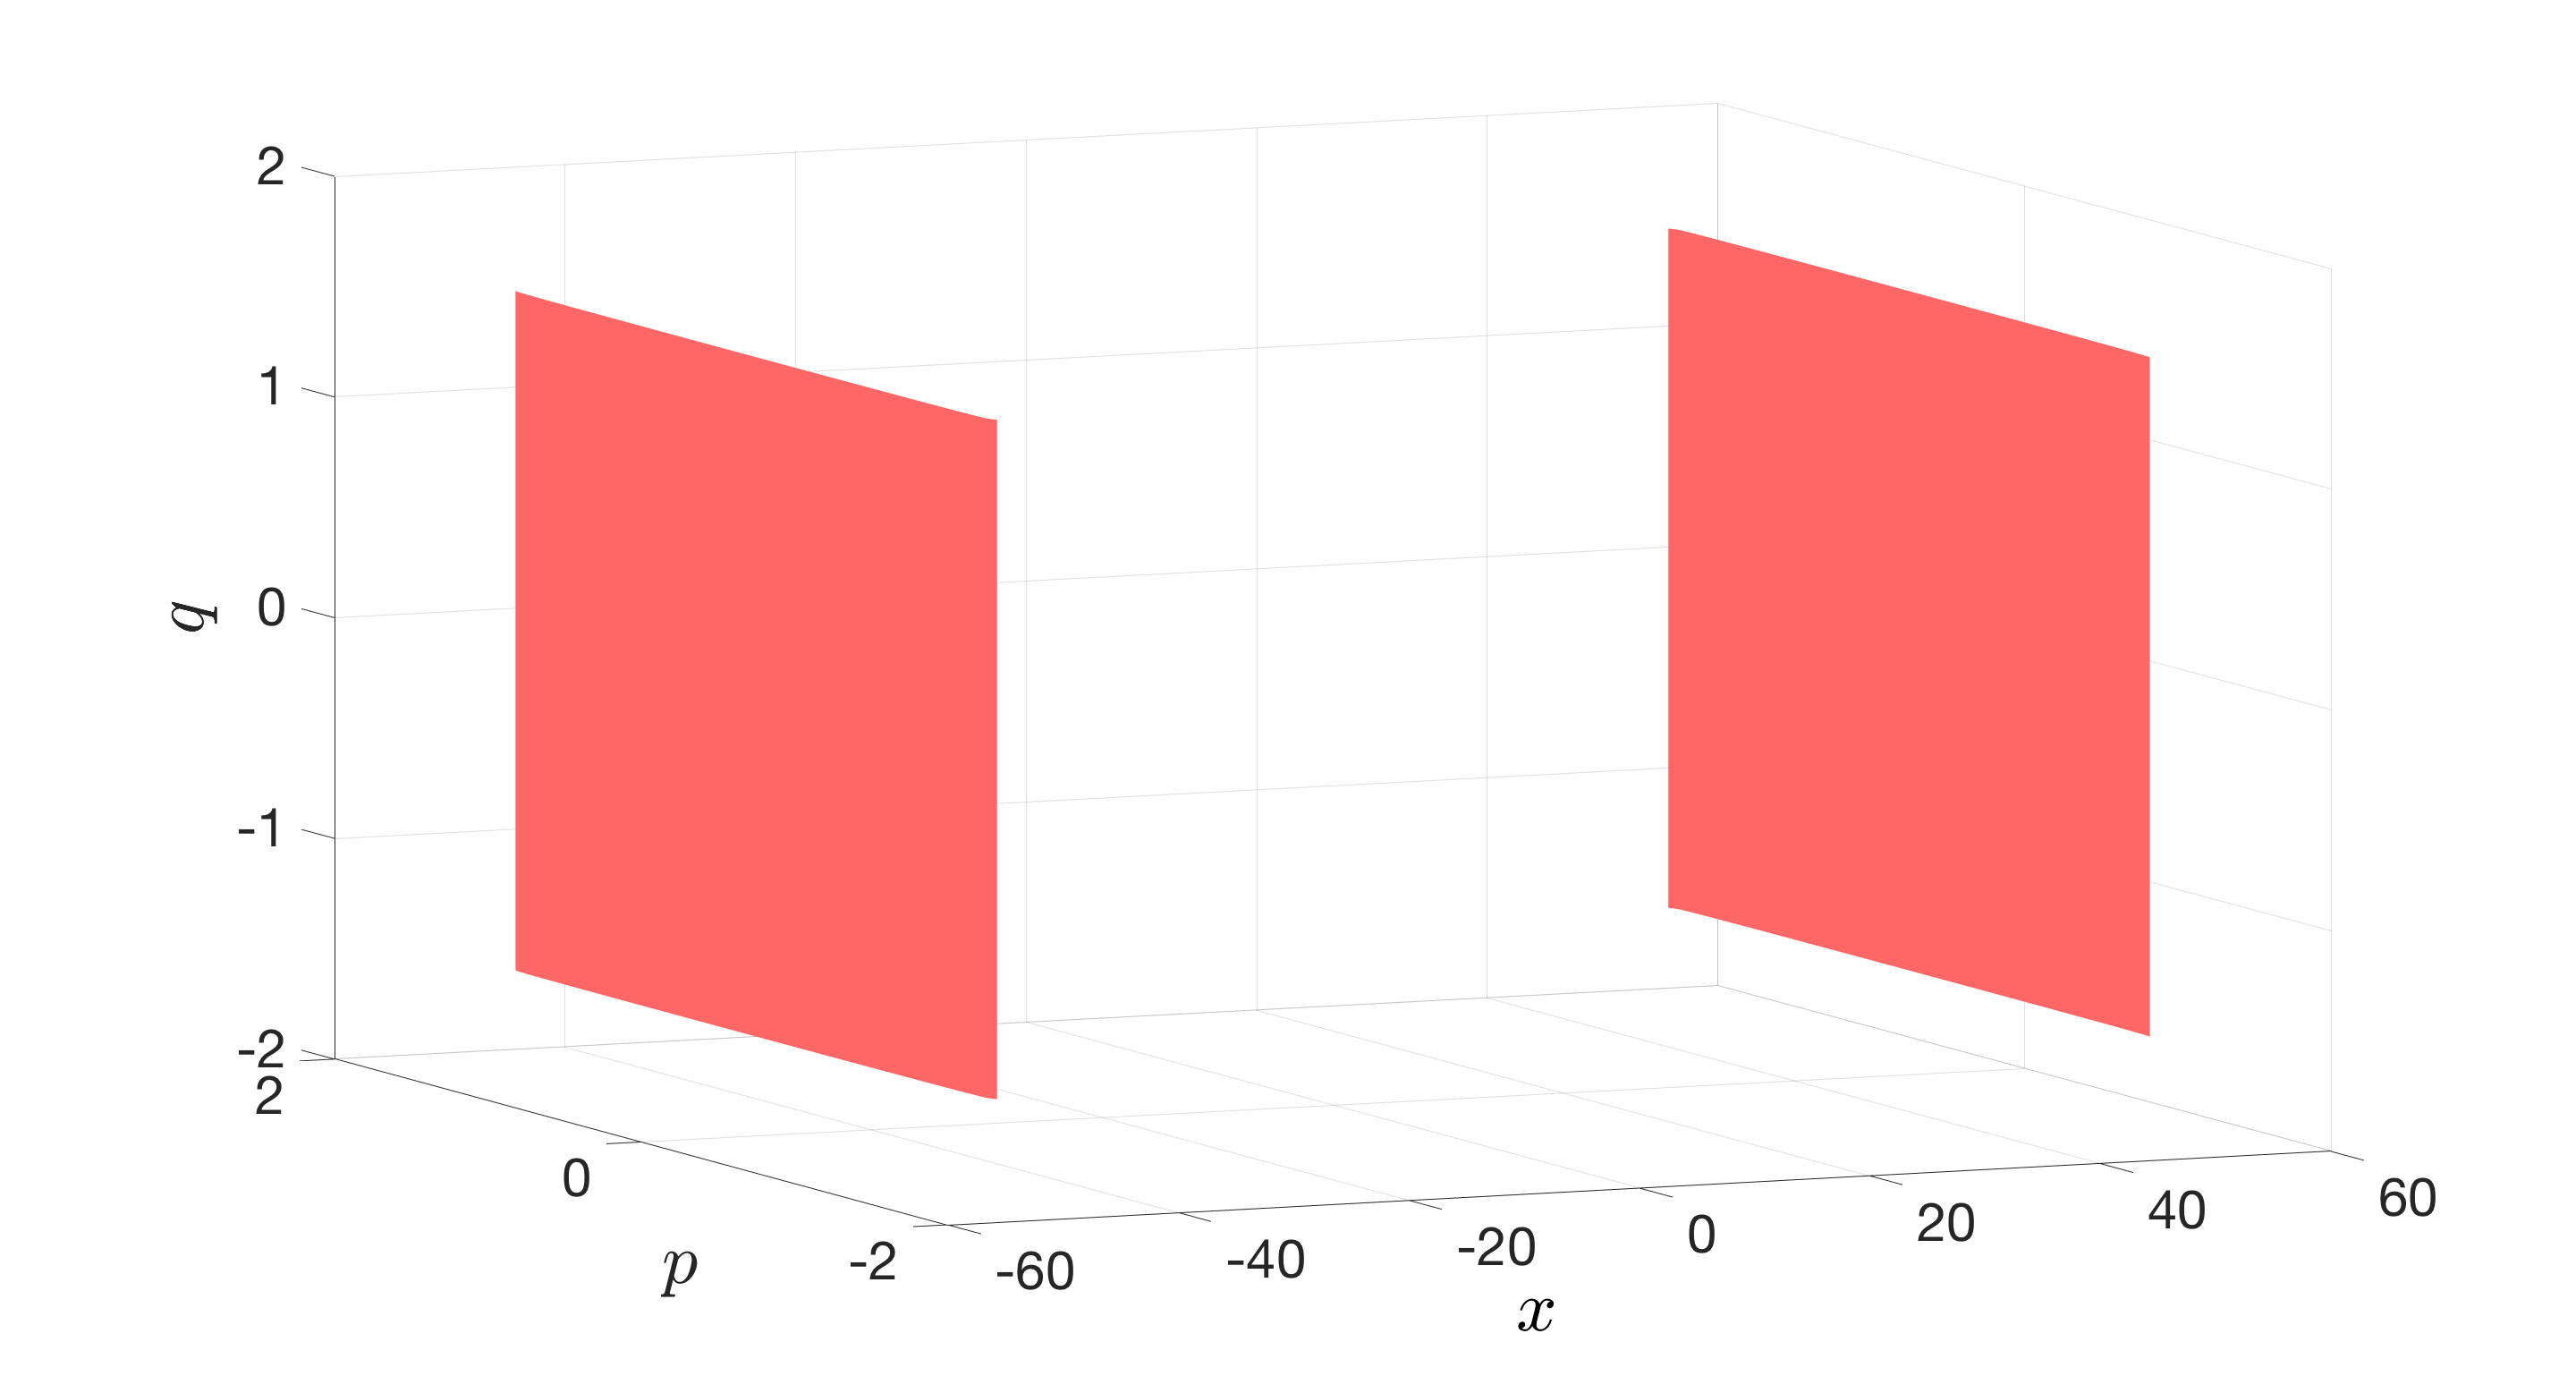
\includegraphics[width=\textwidth]{figures/pen3dred.png}
        \caption{}
        \label{penrosered}
    \end{subfigure}
    \hfill
    \begin{subfigure}[b]{0.45\textwidth}
        \centering
        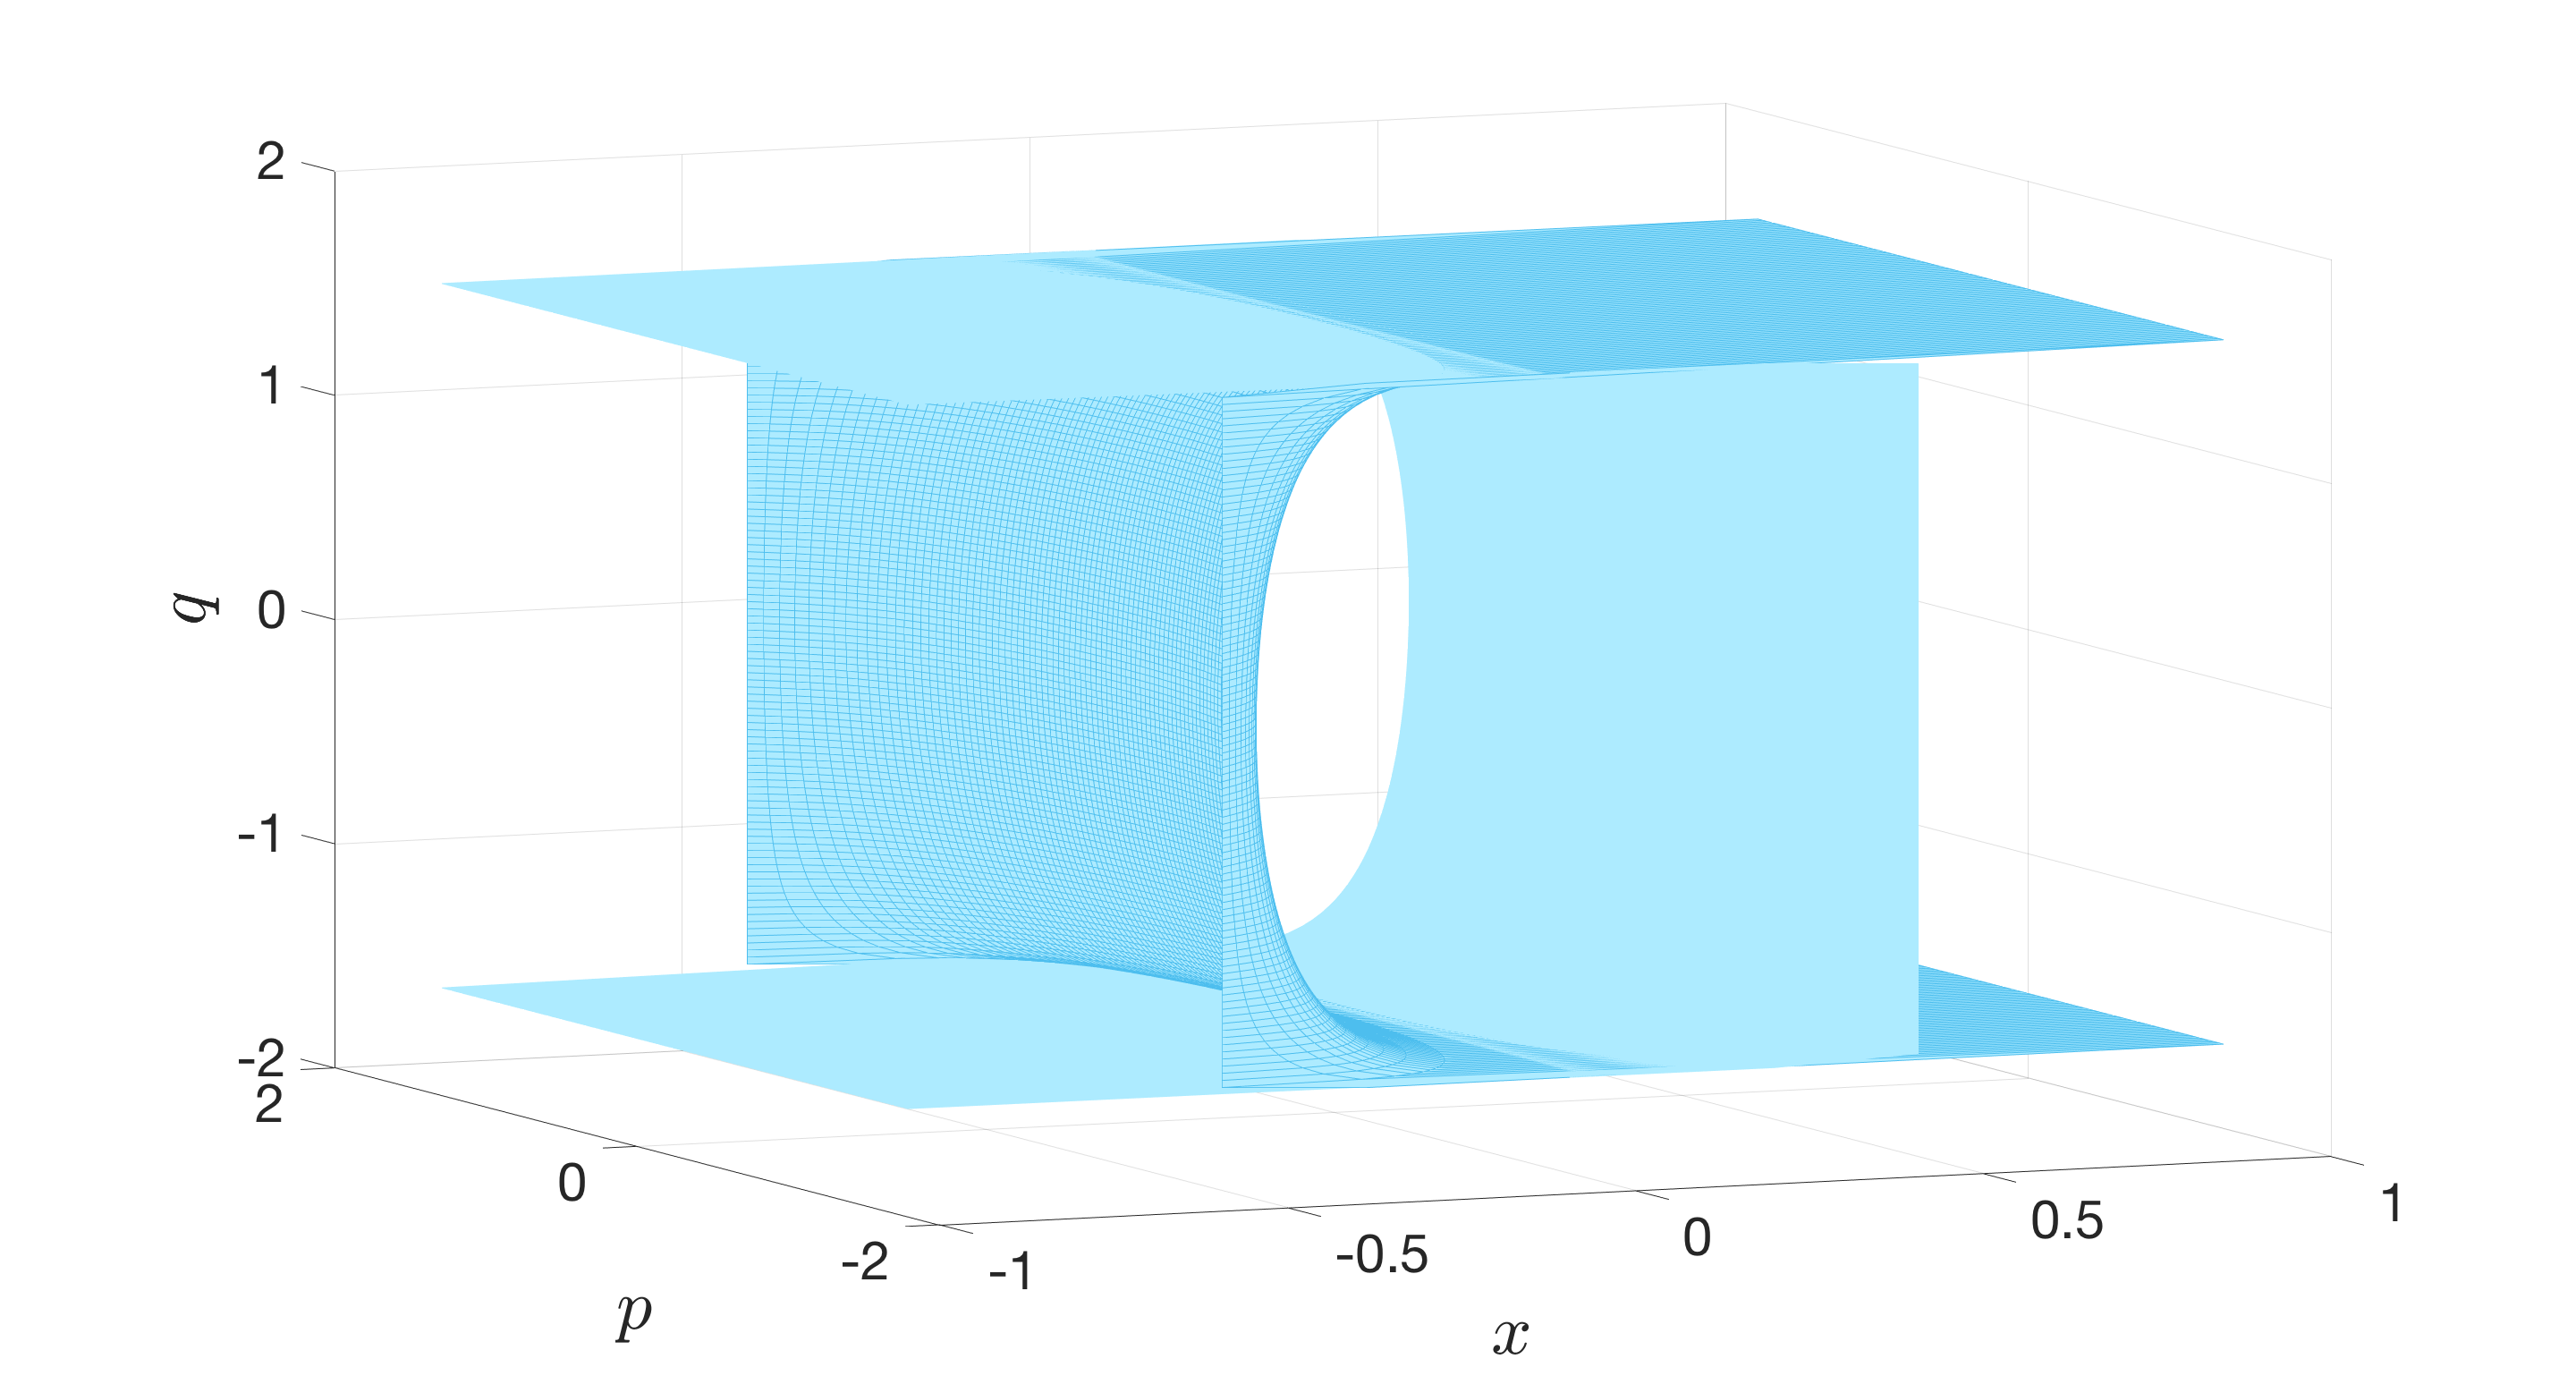
\includegraphics[width=\textwidth]{figures/pen3dblue.png}
        \caption{}
        \label{penroseblue}
    \end{subfigure}
    \caption{3 dimensional Penrose diagrams of the two slices. The two walls diverge at the singularity. While the red slice's walls diverge in different directions, the blue ones diverge towards each other in the $x$ direction which leads to a wall collision near the singularity.}
    \label{penrose3d}
\end{figure}

Since we have an $x$ coordinate that features walls in the hot phase discussed earlier, we would like to add the $x$ axis to the Penrose picture. This will result in a sort of 3 dimensional plots. The wall solution computed in chapter \ref{section 5} can be given in terms of the ($p,q$) coordinates. Using equation (\ref{mysolved}), the wall equation becomes
\begin{equation}
    \alpha_j(p_j,q_j) = \frac{1}{2\pi T}\tanh^{-1}\left(\frac{\ell_j\left(\lambda^2+\epsilon_j{\lambda_0}^2\right)}{2\lambda}\frac{1}{\sqrt{a_j\left(\frac{\cos^2(q_j)}{\cos^2(p_j)}-1\right)+1}}\right) + \frac{L_j}{2},
\end{equation}
where $\epsilon_j=\delta_{j,1}-\delta_{j,2}$. The continuation of the wall solution behind the horizon diverges at the singularity. The two walls seem to collide before reaching this point. The 3D Penrose diagram is represented in \ref{penrose3d}.

We can see from the change of the coordinates (\ref{Penrose coord}) that:
\begin{itemize}
  \item The point $r\to\infty$ corresponds to the point $p=\pm\frac{\pi}{2}$,
  \item The point $r=0$ corresponds to the point $q=\pm\frac{\pi}{2}$,
  \item The point $r=r_h$ corresponds to the point $p=\pm q$.
\end{itemize}

\section{RT surfaces and Page curve}

We can derive a version of the information paradox in the case at hand. The double sided geometry computed in the previous section is dual to an ICFT in a pure state living on the double boundary $M\cup M'$ of fig. \ref{Penrose diagram thermofield double}.

We want to compute time dependant RT surfaces. This can be considered by taking the boundary region to sit in a $q\neq0$ slice. If we move the right side forward, while moving the left side downwards in the $q$ direction, it will leave the state of the system unchanged as it is an isometry. This can also be seen in the case of the thermofield double by evolving the purified state with respect to the Hamiltonian $H = H_1-H_2$, where $H_i$ is the Hamiltonian of the $j^\text{th}$ copy. However, we can move both sides in the upward direction of $q$. Computing RT surfaces in this case gives time dependant entropies.

The RT surfaces in question are those homologous to the double sided interval $\Tilde{A}=A\cup A'$, see fig. \ref{aua'}. There are two possible RT surfaces. The first one is composed of two symmetric surfaces $m(A)$ and $m(A')$ respectively homologous to $A$ and $A'$. The second one is a surface linking a point in $\partial A$ to a point in $\partial A'$ and its symmetric surface linking the two other boundary points. The schematic RT surfaces are represented in fig. \ref{aua'}.

\begin{figure}
    \centering
    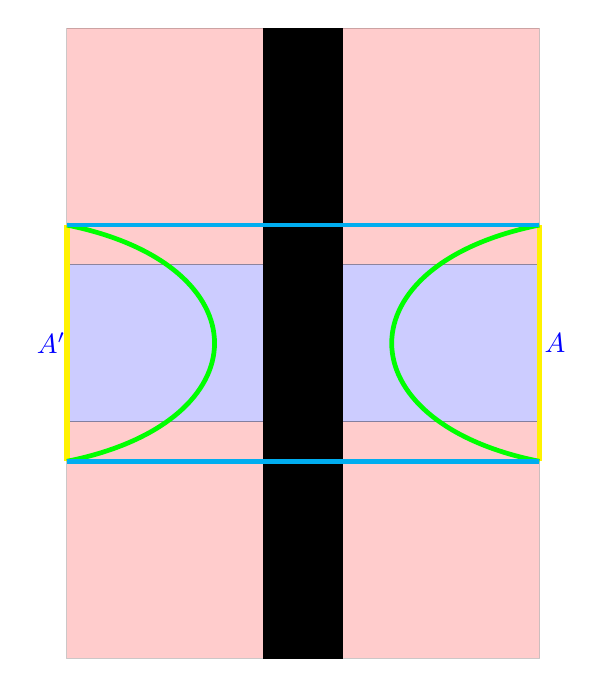
\begin{tikzpicture}
        \draw[black, fill=red, opacity=0.2] (-3,1) -- (3,1) -- (3,4) -- (-3,4) -- (-3,1);
        \draw[black, fill=blue, opacity=0.2] (-3,1) -- (3,1) -- (3,-1) -- (-3,-1) -- (-3,1);
        \draw[black, fill=red, opacity=0.2] (-3,-1) -- (3,-1) -- (3,-4) -- (-3,-4) -- (-3,-1);
        \draw[fill=black] (-.5,4) -- (.5,4) --(.5,-4) -- (-.5,-4) -- (-.5,4);
        \draw[yellow, line width=2] (3,1.5) -- (3,-1.5);
        \draw[yellow, line width=2] (-3,1.5) -- (-3,-1.5);
        \draw[color=green,line width=.6mm] (3,1.5) .. controls (.5,1) and (.5,-1) .. (3,-1.5);
        \draw[color=green,line width=.6mm] (-3,1.5) .. controls (-.5,1) and (-.5,-1) .. (-3,-1.5);
        \draw[color=cyan,line width=.6mm] (3,1.5) -- (-3,1.5);
        \draw[color=cyan,line width=.6mm] (3,-1.5) -- (-3,-1.5);
        \draw[blue] node at (3.2,0){$A$};
        \draw[blue] node at (-3.2,0){$A'$};
    \end{tikzpicture}
    \caption{Representation of constant $q$ slice of the 3d Penrose diagram. The black stripe represents the horizon. At $q=0$ this stripe is a line. We have two possible RT surfaces represented in blue and green.}
    \label{aua'}
\end{figure}

Let's start with green geodesic in figure \ref{aua'}. This geodesic is composed of two symmetric ones, each living in one side of the double geometry. These geodesics are actually the same as that computed in eq. (\ref{S2}). Since the geometry is static in the original coordinates, the RT surfaces remain constant as time flows. The value of this entropy is then,
\begin{equation}
    S_1= 4\ell_1\left(\log\left(\frac{2}{\epsilon}\right)- \log\left({r_h}_1^2\left(1-\tanh(\sqrt{M}(\alpha_1(0)-h/2))\right)\right)\right).
\end{equation}

The blue RT surface links two opposite points on the cutoff surface. These surfaces remain in the red slice and can be computed in the same way as the previous chapter, by considering the 1 dimensional Lagrangian,
\begin{equation}\label{thela Lagrangian}
    L = \ell_1\int\frac{\text{d}p_1}{\cos(p_1)}\,\sqrt{1+M\cos^2(q_1)x_1'^2},
\end{equation}
where the prime denotes a derivative with respect to $p_1$. The Euler-Lagrange equation (rearranged) reads,
\begin{equation}
    x'_1^2\left(\frac{k}{\cos^2(p_1)}-\frac{J^2}{\ell_1}\right)=\frac{J^2}{k},
\end{equation}
where $k=M\ell_1\cos^2(q_1)$ and $J$ is a constant of integration to be determined by boundary conditions. The solution is given by,
\begin{equation}
    x_1(p_1) = \pm \frac{1}{\sqrt{M}\cos(q_1)}\tanh^{-1}\left(\frac{J\sin(p_1)}{\sqrt{k\ell_1-J^2\cos^2(p_1)}}\right) +x_0.
\end{equation}
where $x_0$ is a constant. The symmetry of the geometry implies that the minimal geodesic is the one that remains straight in the $p_1$ direction, i.e constant $x_1$ as drawn in figure \ref{aua'}. This implies that $x_0=x_1(\pi/2-\epsilon(q_1))$ and $J=0$. 

Integrating (\ref{thela Lagrangian}) at fixed $x_1$ gives,
\begin{align}
    L &= \ell_1\int_{-{p_{\epsilon(q_1)}}}^{p_{\epsilon(q_1)}}\frac{\text{d}p_1}{\cos(p_1)}\\
    &= 2\ell_1\cdot\log\left(\tan(p_1)+\frac{1}{\cos(p_1)}\right)\bigg|_{p_{\epsilon(q_1)}}.\\
\end{align}
The time dependence comes from the non trivial cutoff surface ${p_{\epsilon(q_1)}}$. This cutoff surface is found from the Penrose change of coordinates by setting $r=1/\epsilon$. We find\footnote{see appendix \ref{appendix F} for detailed calculations},
\begin{equation}
    \cos({p_{\epsilon(q_1)}}) = \epsilon{r_h}_1\cos(q_1).
\end{equation}

\begin{figure}
    \centering
    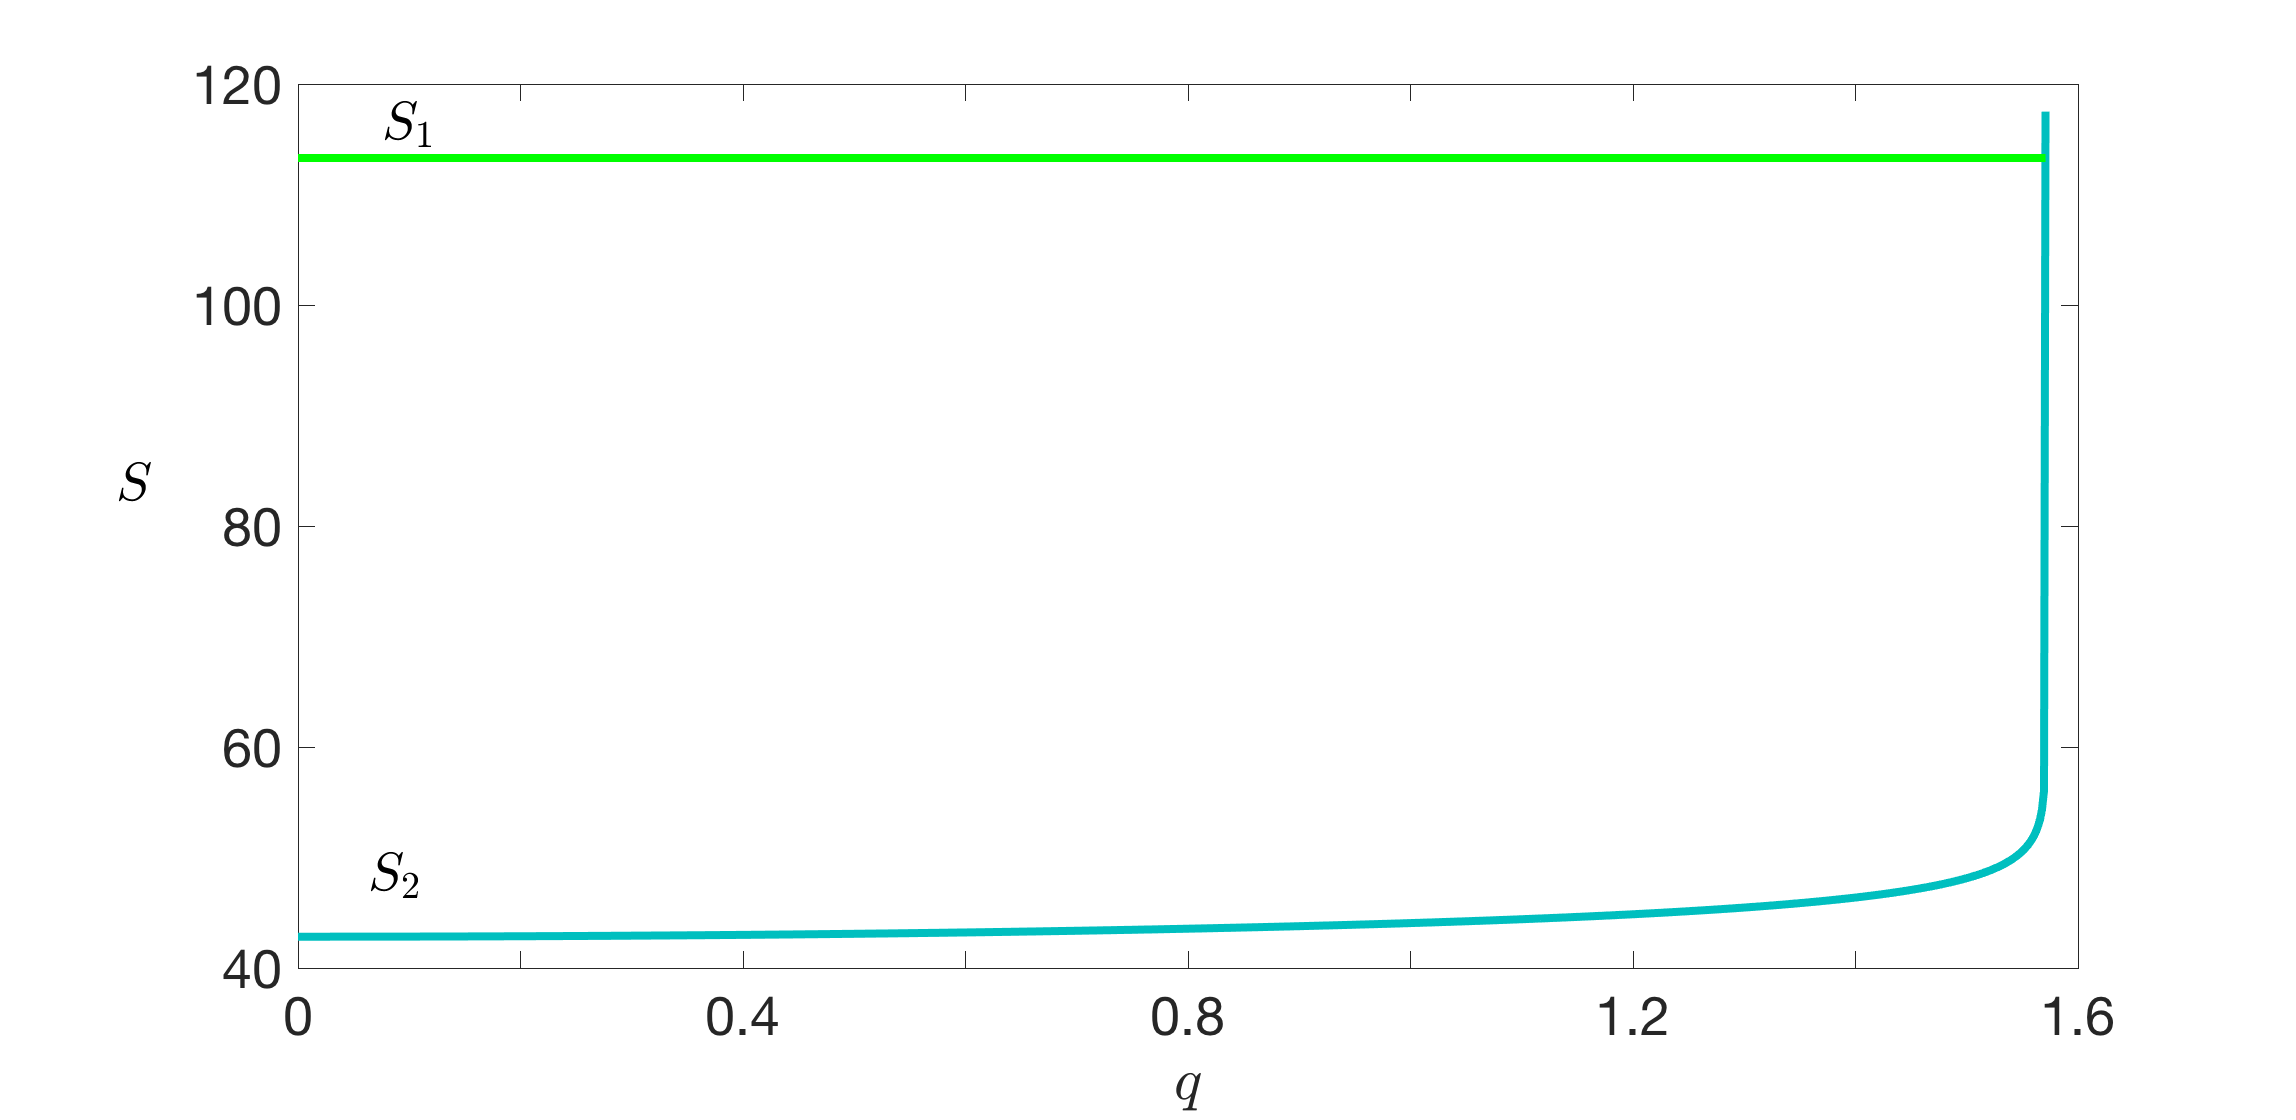
\includegraphics[width=1\textwidth]{figures/Page_thing.png}
    \caption{The entropy $S$ of the boundary interval $\Tilde{A}$ given by equation (\ref{final entropy}). We see a rising entropy $S_2$ at the beginning, however it crosses the value of $S_1$ at a finite Page time.}
    \label{the final Page curve}
\end{figure}


Putting all of this together, we find the length of the RT surface, as we expand around $\epsilon=0$, to be
\begin{equation}\label{c'est bon}
    S_2(q_1) = 4\ell_1\log\left(\frac{2}{\epsilon {r_h}_1\cos(q_1)}\right).
\end{equation}
This entropy is an increasing function of $q_1$ and therefore an increasing function of $t$. In fact we can express $S_2(q_1)$ as a function of the real time instead using,
\begin{equation}
    \cos(q_1)=\sqrt{\frac{1-\epsilon^2{r_h}_1^2\tanh^2\left(\frac{{r_h}_1t}{\ell_1}\right)}{1-\epsilon^4{r_h}_1^4\tanh^2\left(\frac{{r_h}_1t}{\ell_1}\right)}}.
\end{equation}
This is shown in appendix \ref{appendix F}.

The final entropy is the minimal of the two,
\begin{equation}\label{final entropy}
    S(\Tilde{A}) = \min\left\{S_1,S_2(q_1)\right\}.
\end{equation}

We plotted the entropy as a function of time in figure \ref{the final Page curve}. We see that the entropy starts rising at first, until it reaches the constant value $S_1$ which saturates the entropy and remains constant for the rest of time.

This entropy growth given by $S_2$ is similar to Hawking's information paradox since it surpasses the coarse grained entropy at the Page time. This infinite growth contradicts the finite number of states of the boundary QM system. We solve this paradox by means of the other RT surface $S_1$. We suspect that the result should remain the same in the case of multiple slices inside the blue slice as long as the their corresponding central charges remains larger than that of the exterior slice.




\addchap{Conclusion}\label{section 8}
\setcounter{chapter}{8}
In this note we started with a general system with 2 CFTs separated with an interface. This system extends to gravitational solutions in the bulk separated by a domain wall. We were interested in the case where one slice has larger degrees of freedom to model something close to a black hole following the central Dogma. In this limit (as well as large boundary for the other slice), we found that the dominant phase is the hot phase with a part of the horizon on each side. The geometry was computed explicitly in the case of $[\text{H}2,\text{H}2]$. 

We then computed RT surfaces in the single sided geometry. This problem turned out to be computations of space-like geodesics as the metric is time independant. As we take the limit of large boundary in the red slice, the true RT surface is the one that crosses the wall. The latter is $\sigma$ dependant geodesic. The large $\ell_2$ limit considered implies that the true geodesic is that close to the horizon, $\sigma=0$.

We finally discussed a version of the Hawking information paradox involving a two-sided hot phase staring in the Hartle-Hawking state, and evolved forward in time on both sides. We computed RT surfaces homologous to the boundary subregion $\Tilde{A}$. One geodesic was found to be a increasing function of time, which is a version of Hawking's information paradox. A second RT surface was found to be constant over time, and therefore takes over the first entropy as we take the minimum of the two. This RT surface is complicated to compute in the double sided geometry as it can move in the $q$ direction as well. However, it can be computed in the original one sided geometry since it consists of two parts, each remaining in its corresponding side.

This study is similar to the work presented in \cite{almheiri2019islands}. Our system is $2+1$ dimensional and spiced with a wall separating two geometries. However, the result of the final entropy in this example stays consistent with the literature discussed above.


\textbf{Acknowledgment}

I would like to thank Prof. João Penedones for his assistance and his helpful advice.
I would also like to thank Kelian Häring for allowing me to push forward
during this Thesis.


% \appendix
% \addchap{Appendix}
% \setcounter{chapter}{A}
% \input{app.tex}

\appendix
\addchap{Appendix A}
\setcounter{chapter}{0}
\refstepcounter{chapter}
\label{appendix A}
This Appendix refers to chapter \ref{section 2}. We detail some computations that we believe to be important for a complete report.

\section{Bell state}

Consider the Bell state (\ref{Bell pair}). The reduced density matrix matrix was found by tracing over $B$ and is given in (\ref{psiA}). From $\rho_A$ we find,
\begin{equation}
    \rho\ln\rho= \frac{\ln(2)}{2}\left(\ket{0}_A\bra{0}+\ket{1}_A\bra{1}\right).
\end{equation}
Plugging this in the definition of von Neumann entropy, we find
\begin{equation}
    S = \ln(2).
\end{equation}
This shows that $A$ and $B$ are maximally entangled.

\section{Strong Subadditivity}
The strong subadditivity condition (\ref{weak monotonicity}) can be rewritten by mean of the conditional entropy,
\begin{align}
    S\left(AB\right) + S\left(BC\right) \geq S\left(A\right) + S\left(C\right) &\implies S\left(AB\right) -  S\left(A\right)  + S\left(BC\right)-S\left(C\right)\geq 0\\
    &\implies H\left(B|A\right) + H\left(B|C\right)\geq 0.
\end{align}

\section{thermofield double}

In this appendix we check using path integrals that tracing over the system $B$ in equation \ref{thermofield double} gives back the original Gibbs state. 
\begin{align}
    _A\bra{x_0}\text{Tr}_B\left(\rho=\ket{\phi}\bra{\phi}\right)\ket{x_1}_A &= \int\text{d}y\bra{x_0,y}\ket{\phi}\bra{\phi}\ket{x_1,y}\\
    &= \frac{1}{Z}\int\text{d}y ~~ \ctikz{\draw (-1,-0.15) arc (190:350:1);\node at (-1,-0.15) [circle,fill=red,inner sep=1.5pt]{}; \node at (1,-0.15) [circle,fill=red,inner sep=1.5pt]{};
    \draw node at (-1.3,-0.15){$y$};\draw node at (1.3,-0.15){$x_0$};\draw node at (-1.3,0.15){$y$};\draw node at (1.3,0.15){$x_1$}; \draw (1,0.15) arc (10:170:1);\node at (-1,0.15) [circle,fill=red,inner sep=1.5pt]{}; \node at (1,0.15) [circle,fill=red,inner sep=1.5pt]{};}\\
    &= \frac{1}{Z} \cdot \ctikz{\draw (0.967,0.255) arc (10:350:1);\node at (0.967,0.255) [circle,fill=red,inner sep=1.5pt]{}; \node at (0.96,-0.150) [circle,fill=red,inner sep=1.5pt]{};
    \draw node at (1.3,-0.2){$x_0$};\draw node at (1.3,0.2){$x_1$};},
\end{align}
which is exactly the Gibbs state from the definition \ref{l3iba}.

\appendix
\addchap{Appendix B}
\setcounter{chapter}{1}
\refstepcounter{chapter}
\label{appendix B}
This Appendix refers to chapter \ref{section 3}.

\section{Geodesics in AdS space time}

In this section, we compute space like geodesics inside AdS space time in 2+1 dimension.The geometry is explicitly described in equation \ref{AdS_3 metric}. In static geometries we are interested in space like geodesics to compute RT surfaces. The metric of interest becomes,
\begin{equation}\label{static ads}
    \text{d}s^2= \frac{\ell^2}{z^2}\left(\text{d}x^2+\text{d}z^2\right).
\end{equation}

Geodesics can be found by solving Einstein field equations or simply by treating the metric \ref{static ads} as a one dimensional Lagrangian,
\begin{equation}\label{Lagr}
    L = \int\frac{\text{d}x}{z}\sqrt{\dot z^2+1}.
\end{equation}
The dot correspond to a derivative with respect to $x$. As the Lagrangian is time independent, the energy conservation reads,
\begin{equation}
    E = \frac{1}{z\sqrt{\dot z^2+1}}.
\end{equation}
The solutions of this differential equation is,
\begin{equation}
    z = \pm \sqrt{E^{-2}-(x-x_0)^2},
\end{equation}
where $x_0$ is a constant of integration. This can be rearranged in as written in eq. (\ref{AdS_3 vaccum geodesic}) with $r=\frac{1}{E}$.

Plugging this solution back in eq. (\ref{Lagr}), we find the length of the geodesic,
\begin{align}
    L &= 2r\ell \int_0^\frac{L}{2} \text{d}x ~ \frac{1}{z^2}\\
    &= 2r \int_0^\frac{L}{2} \text{d}x ~ \frac{1}{(x-x_0)^2-r^2}\\
    &= \log\left(\frac{r+x-x_0}{r-x+x_0}\right)\Big|^\frac{L}{2}.
\end{align}
Replacing with $x_0 = 0$ and $r^2 = \left(\frac{L}{2}\right)^2+\epsilon^2$ we get exactly eq. (\ref{first RT}).

\section{Hawking temperature}

Consider the metric (\ref{BTZ}) with the change of coordinate $z=1/r$,
\begin{equation}
    \text{d}s^2 = \ell^2\left(-g\left(r\right)\text{d}t^2+\text{d}x^2+\frac{\text{d}r^2}{g\left(r\right)}\right),
\end{equation}
where $g(r) = r^2-r_h^2$ with $r_h=1/z_h$.

By making a Wick rotation $\tau=it$ we get the Euclidean geometry,
\begin{equation}
    \text{d}s^2 = \ell^2\left(g\left(r\right)\text{d}\tau^2+\text{d}x^2+\frac{\text{d}r^2}{g\left(r\right)}\right).
\end{equation}
Near the horizon we can rewrite the metric by expanding $g(r)$ around $r_h$. We make the following change of coordinate,
\begin{align}
    (r-r_h)=\frac{1}{4}g'(r_h)\rho^2, && \tau = \frac{\beta}{2\pi}\theta,
\end{align}
where $\beta$ is the period of $\tau$. The metric becomes,
\begin{equation}
    \text{d}s^2 = \ell^2\left(\left(\frac{g'(z_h)\beta}{4\pi}\right)^2\text{d}\tau^2+\text{d}x^2+\text{d}\rho^2\right).
\end{equation}

In order to avoid the conical singularity at $r=r_h$, we need to take the factor multiplying $\text{d}\theta$ to be 1. The point at the horizon shouldn't be something special compared to the rest of space-time outside the horizon.
\begin{equation}
    \frac{g'(z_h)\beta}{4\pi} = 1\implies T = \frac{r_h}{2\pi} = \frac{1}{2\pi},
\end{equation}
where $\beta = \frac{1}{T}$.

\appendix
\addchap{Appendix C}
\setcounter{chapter}{2}
\refstepcounter{chapter}
\label{appendix C}
This Appendix refers to chapter \ref{section 5}.

\section{The range of the tension of the wall}


\section{Boundary conditions}

The boundary conditions (\ref{Dirichelet bc}) can be rewritten for the warm phases with centerless blue slices as,
\begin{equation}
    2\pi\tau_2 = -\sqrt{M_1}\frac{\ell_2}{\sqrt{A}} {\int_{\sigma_+}}^\infty \text{d}\sigma\, \frac{\sigma\left(\lambda^2-{\lambda_0}^2\right)+M_2-M_1}{\left(\sigma+M_2{\ell_2}^2\right)\sqrt{\sigma\left(\sigma-\sigma_+\right)\left(\sigma-\sigma_-\right)}}.
\end{equation}
We make a change of coordinates $s = \sigma/M_1$,
\begin{equation}\label{eq2}
    2\pi\tau_2 = -\frac{\ell_2}{\sqrt{A}} {\int_{s_+}}^\infty \text{d}s\, \frac{s\left(\lambda^2-{\lambda_0}^2\right)+\mu-1}{\left(s+\mu{\ell_2}^2\right)\sqrt{s\left(s-s_+\right)\left(s-s_-\right)}}.
\end{equation}
In the same way, the red side boundary condition takes the form,
\begin{equation}\label{eq1}
    2\pi T\Delta x_1\big|_\text{Hor}-2\pi\tau_1 = \frac{\ell_1}{\sqrt{A}} {\int_{s_+}}^\infty \text{d}s\, \frac{s\left(\lambda^2+{\lambda_0}^2\right)-\mu+1}{\left(s+{\ell_1}^2\right)\sqrt{s\left(s-s_+\right)\left(s-s_-\right)}}.
\end{equation}
The LHS of eq. (\ref{eq2}) and (\ref{eq1}) are the functions $-\Tilde{f}_2(\mu)$ and $\Tilde{f}_1(\mu)$ referred to in eq. (\ref{f2 constrain}). As discussed in chapter \ref{section 5}, these functions can be written in terms of the elliptic integrals of the first, second and third kind,
\begin{align}
    \bm{K}(\nu) &= \int_{0}^{1} \frac{\mathrm{d}t}{\sqrt{\left(1 - t^2\right)\left(1 - \nu^2 t^2\right)}},\\
    \bm{E}(\nu) &= \int_0^1 \frac{\sqrt{1-\nu^2 t^2} }{\sqrt{1-t^2}}\,\mathrm{d}t,\\
    \bm{\Pi}(u,\nu) &= \int_{0}^{1} \frac{1}{1-ut^2} \frac{\mathrm{d}t}{\sqrt{\left(1-\nu t^2\right)\left(1-t^2\right)}}.
\end{align}

We make the change of coordinates $t^2=s_+/s$ and plug it in (\ref{eq2}),
\begin{equation}\label{eq22}
    \Tilde{f}_2(\mu) = \frac{2\ell_2}{\sqrt{As_+}} {\int_{0}}^1 \text{d}t\,\frac{t^2}{s_+} \frac{\frac{s_+}{t^2}\left(\lambda^2-{\lambda_0}^2\right)+\mu-1}{\left(1+\frac{\mu{\ell_2}^2}{s_+}t^2\right)\sqrt{\left(1-t^2\right)\left(1-\frac{s_-}{s_+}t^2\right)}}.
\end{equation}
We make the following change $s_\pm=\sigma_\pm/M_1$, $\nu=s_-/s_+s$ and $u=-\mu\ell_2^2/s_+$. We get
\begin{equation}
    \Tilde{f}_2(\mu) = \frac{2\ell_2}{\sqrt{As_+}}\left[\frac{1-\mu}{s_+ u}\left(\bm{K}(\nu)-\bm{\Pi}(u,\nu)\right)+\left(\lambda^2-\lambda_0^2\right)\bm{\Pi}(u,\nu)\right].
\end{equation}

\appendix
\addchap{Appendix D}
\setcounter{chapter}{3}
\refstepcounter{chapter}
\label{appendix D}
This Appendix refers to chapter \ref{section 6}.

\section{Constants of integration}

We start by deriving eq. (\ref{maconstante}). For geodesic $\gamma_1$ in the red slice we chose to parametrise our paths with respect to $r_1$ rather than $x_1$. The action computed in eq. (\ref{Action}) becomes,
\begin{equation}\label{Aaction}
    L = \ell\int d r\sqrt{\frac{1}{r^2-M\ell^2}+r^2\phi'^2}.
\end{equation}
Treating $L$ as a one dimensional action, the Euler-Lagrange equation gives,
\begin{equation}
    \frac{r^2\phi'}{\sqrt{\frac{1}{r^2-M\ell^2}+r^2\phi'^2}}= \frac{J}{\ell},
\end{equation}
where $J$ is a constant of integration. Rearranging this equation, we get,
\begin{equation}
    r^2\phi'^2(r^2-J^2/\ell^2)(r^2-r_h^2)=\frac{J^2}{\ell^2},
\end{equation}
where $r_h=\ell\sqrt{M}$. Integrating this equation a second time gives
\begin{equation}\label{therealsol}
    x(r) = \pm\frac{\ell_1}{r_h_1}\tanh\left(\frac{J_1}{r_h_1}\sqrt{\frac{r_1^2-r_h_1^2}{r_1^2\ell_1^2-J_1^2}}\right) + c_1
\end{equation}
where $c_1$ is a constant of integration. We recovered the indices to make our point clear that we are in the red slice.

The $\gamma_1(\sigma)$ geodesic has the following boundary conditions,
\begin{align}
    x_1(1/\epsilon) = \frac{A}{2} = \frac{L_1-h}{2}, && x_1(r_1(\sigma)) = \alpha_1(\sigma).
\end{align}

Plugging these boundary conditions in the solution (\ref{therealsol}), we find,
\begin{align}
    \frac{A}{2} &= \frac{\ell_1}{r_h_1}\tanh\left(\frac{J_1}{r_h_1}\right) + c_1,\\
    \alpha_1(\sigma) &= \frac{\ell_1}{r_h_1}\tanh\left(\frac{J_1}{r_h_1}\sqrt{\frac{\sigma}{\sigma+r_h_1^2\ell_1^2-J_1^2}}\right) + c_1,
\end{align}
where we considered the positive solution $x_1\geq0$. Taking the difference of the two equations, and rearranging a bit, we find,
\begin{equation}
    \tanh \left( {r_h}_1 \frac{2x_1(\sigma) - A}{2\ell_1}\right) = \frac{C(\sigma)-D(\sigma)}{1-C(\sigma)D(\sigma)},
\end{equation}
with the functions $C(\sigma)$ and $D(\sigma)$ given in eq (\ref{CD}). The solution is,
\begin{equation}
    J_1(\sigma) = \frac{\beta r_h_1^3 + \beta r_h_1 \sigma + \sqrt{
\beta^2 r_h_1^4 \sigma - \beta^4 r_h_1^4 \sigma + \beta^2 r_h_1^2 \sigma^2 - 
  \beta^4 r_h_1^2 \sigma^2}}{r_h_1^2 + \beta^2 \sigma},
\end{equation}
where $\beta$ is given by,
\begin{equation}
    \beta = \tanh\left( {r_h}_1 \frac{2x_1(\sigma) - A}{2\ell_1}\right).
\end{equation}

For the case of $\gamma_2(\sigma)$, we used the solution (\ref{solution phi}). The boundary conditions are symmetric in this case,
\begin{align}
    r_2(\sigma) = r_2(-\sigma) = \frac{E_2}{{r_h}_2}\frac{1}{\sqrt{\frac{E_2^2}{r_h_2^2\ell_2^2}\cosh^2\left(r_h_2\frac{\pm x_2(\sigma)}{\ell_2}+c_2\right)-\sinh^2\left(r_h_2\frac{\pm x_2(\sigma)}{\ell_2}+c_2\right)}}.
\end{align}
This implies that $c_2=0$. Inverting this equation for $E_2$, we get,
\begin{equation}
    E_2 = {r_h}_2\sinh\left(r_h_2\frac{ x_2(\sigma)}{\ell_2}\right) \sqrt{\frac{\sigma+{r_h}_2^2}{\frac{\sigma+{r_h}_2^2}{\ell_2^2}\cosh^2\left(r_h_2\frac{ x_2(\sigma)}{\ell_2}\right)-1}}.
\end{equation}

\appendix
\addchap{Appendix E}
\setcounter{chapter}{4}
\refstepcounter{chapter}
\label{appendix E}
This Appendix refers to chapter \ref{section 7}.

\section{Cutoff surface}

The cutoff surface in the $(q,p)$ coordinates is not a trivial surface at constant $p$. It is rather a $(q,p)$ dependant surface. To find this surface we have to map $r$ to $(q,p)$ through (\ref{Kruskal coord}) and (\ref{Penrose coord}),
\begin{equation}
    r = r_h\frac{\cos(q)}{\cos(p)}.
\end{equation}
Then the cutoff surface is given by,
\begin{equation}\label{cutoff}
    \frac{1}{\epsilon} = r_h\frac{\cos(q)}{\cos(p)}\implies \cos(p)=\epsilon r_h \cos(q).
\end{equation}

\section{$q$ to $t$ at the cutoff}

We want to recover the time dependence of the RT surface in eq. (\ref{c'est bon}). Using (\ref{Kruskal coord}) we find,
\begin{equation}
    \frac{v}{u} = \tanh\left(\frac{r_h t}{\ell}\right).
\end{equation}

And from (\ref{Penrose coord}), we find,
\begin{align}
    \frac{v}{u} &= \frac{\sin(q)\cos(q)}{\sin(p)\cos(p)}\\
    &= \frac{1}{\epsilon r_h}\sqrt{\frac{1-\cos^2(q)}{1-\epsilon^2r_h^2\cos^2(q)}},
\end{align}
where we used (\ref{cutoff}).

Rearranging these two equations gives an expression for $\cos(q)$
\begin{equation}
    \cos(q)=\sqrt{\frac{1-\epsilon^2r_h^2\tanh^2\left(\frac{r_h t}{\ell}\right)}{1-\epsilon^4r_h^4\tanh^2\left(\frac{r_h t}{\ell}\right)}}.
\end{equation}



\bibliography{biblio}


\end{document}